% Analysis Note: R_b, R_c, A_FB^b at the Z Pole — Doc 4a (Expected Results)
%
% Compiled with: cd analysis_note && tectonic ANALYSIS_NOTE_doc4a_v1.tex
% All numbers from analysis_note/results/*.json (single source of truth).

\documentclass[11pt,a4paper]{article}
\usepackage[margin=0.75in]{geometry}

% --- Standard preamble (do not modify) ---
\input{../conventions/preamble.tex}

% --- Additional packages for direct LaTeX writing ---
\usepackage{amsmath}
\usepackage{amssymb}
\usepackage{booktabs}
\usepackage{hyperref}
\usepackage{cleveref}
\usepackage{xcolor}
\usepackage{subcaption}
\usepackage{lineno}
\linenumbers

% --- Placeholder command for future-phase values ---
\newcommand{\tbd}[1]{\textcolor{gray}{\textit{#1}}}

% --- Input provenance markers ---
\newcommand{\measured}[1]{\textcolor{blue}{#1}}
\newcommand{\external}[1]{\textcolor{red}{#1}}

% --- Bibliography ---
\bibliographystyle{unsrt}

% =====================================================================
% METADATA
% =====================================================================
\title{Analysis Note: Measurement of $R_b$, $R_c$, and $A_\mathrm{FB}^b$\\
in Hadronic $Z$ Decays Using ALEPH Open Data}
\author{JFC Autonomous Analysis Framework}
\date{Powered by Claude Code \quad$\cdot$\quad \today}

\begin{document}
\maketitle

% =====================================================================
% ABSTRACT
% =====================================================================
\begin{abstract}
The hadronic partial width ratios $R_b = \Gamma(Z \to b\bar{b})/\Gamma(Z \to \mathrm{hadrons})$
and $R_c = \Gamma(Z \to c\bar{c})/\Gamma(Z \to \mathrm{hadrons})$, together with the
$b$-quark forward-backward asymmetry $A_\mathrm{FB}^b$, are measured using $2.89 \times 10^6$
hadronic $Z$ decays collected by the ALEPH detector at LEP at $\sqrt{s} \approx 91.2$~GeV.
The analysis employs a double-tag hemisphere counting method for $R_b$ with a combined
lifetime-probability and invariant-mass tag, and a hemisphere jet charge method for
$A_\mathrm{FB}^b$ at five momentum-weighting parameters $\kappa = 0.3, 0.5, 1.0, 2.0, \infty$.
$R_c$ is constrained to its Standard Model value.
This document presents expected results from Monte Carlo pseudo-data (Phase~4a):
$R_b = 0.280 \pm 0.031\;\mathrm{(stat)} \pm 0.395\;\mathrm{(syst)}$
(a self-consistency diagnostic of the circular calibration procedure),
$A_\mathrm{FB}^b = -0.0001 \pm 0.002\;\mathrm{(stat)} \pm 0.004\;\mathrm{(syst)}$
(correctly zero on symmetric MC), and
$\sin^2\theta_\mathrm{eff}^\mathrm{lept} = 0.250 \pm 0.0004\;\mathrm{(stat)}$.
Observed results on data will be added in subsequent phases (Doc~4b/4c).
\end{abstract}

\tableofcontents
\clearpage

% =====================================================================
% CHANGE LOG
% =====================================================================
\section*{Change Log}
\addcontentsline{toc}{section}{Change Log}

\textbf{Doc 4a v1}
\begin{itemize}
\item Initial analysis note version (expected results only, MC pseudo-data).
\item Full 13-section structure established.
\item 36 figures staged from Phases 1, 3, and 4a.
\item Systematic evaluation complete: 12 sources for $R_b$, 4 sources for $A_\mathrm{FB}^b$.
\item Closure tests, cross-checks, and precision investigation documented.
\end{itemize}

\clearpage

% =====================================================================
% 1. INTRODUCTION
% =====================================================================
\FloatBarrier
\needspace{4\baselineskip}
\section{Introduction}
\label{sec:intro}

At the $Z$ pole, the partial width ratios $R_b^0 = \Gamma(Z \to b\bar{b})/\Gamma(Z \to \mathrm{hadrons})$
and $R_c^0 = \Gamma(Z \to c\bar{c})/\Gamma(Z \to \mathrm{hadrons})$ provide precision tests of
the electroweak vertex corrections coupling the $Z$ boson to heavy quarks.
$R_b$ is sensitive to the top quark mass through $Zb\bar{b}$ vertex corrections involving
the large $V_{tb}$ CKM coupling, making it a probe of non-standard physics at the
$Zb\bar{b}$ vertex even with $m_t$ precisely known~\cite{ALEPH:Rb:1996, LEP:EWWG:2005}.
Most QCD and electroweak radiative corrections cancel in the ratio, leaving $R_b$
with a clean sensitivity to vertex effects.

The $b$-quark forward-backward asymmetry $A_\mathrm{FB}^b$ measures the parity violation
in $Z \to b\bar{b}$ through the product of initial-state and final-state couplings.
At tree level:
\begin{equation}
A_\mathrm{FB}^{0,b} = \frac{3}{4} A_e A_b,
\label{eq:afb_tree}
\end{equation}
where
\begin{equation}
A_f = \frac{2 v_f a_f}{v_f^2 + a_f^2}
\label{eq:asymmetry_param}
\end{equation}
and $v_f$, $a_f$ are the vector and axial-vector couplings of fermion $f$ to the $Z$ boson.
$A_\mathrm{FB}^{0,b}$ provides a determination of the effective weak mixing angle
$\sin^2\theta_\mathrm{eff}^\mathrm{lept}$.  The LEP/SLD combined value of $A_\mathrm{FB}^{0,b}$
shows a 2.8-sigma tension with the SLD $A_\ell$ measurement~\cite{LEP:EWWG:2005},
making this observable of particular interest for probing the consistency of the
Standard Model at the $Z$ pole.

The definitive measurements of $R_b$, $R_c$, and $A_\mathrm{FB}^b$ at the $Z$ pole
were performed by the four LEP experiments and SLD, combined by the LEP Electroweak
Working Group~\cite{LEP:EWWG:2005}:
$R_b^0 = 0.21629 \pm 0.00066$,
$R_c^0 = 0.1721 \pm 0.0030$,
$A_\mathrm{FB}^{0,b} = 0.0992 \pm 0.0016$.
The Standard Model predictions are
$R_b^\mathrm{SM} = 0.21578$,
$R_c^\mathrm{SM} = 0.17223$,
$A_\mathrm{FB}^{0,b,\mathrm{SM}} = 0.1032$~\cite{LEP:EWWG:2005}.

The ALEPH-specific reference measurements are:
$R_b = 0.2158 \pm 0.0009\;\mathrm{(stat)} \pm 0.0011\;\mathrm{(syst)}$ using
a 5-tag double-tag method~\cite{ALEPH:Rb:1996},
$A_\mathrm{FB}^b = 0.0927 \pm 0.0039\;\mathrm{(stat)} \pm 0.0034\;\mathrm{(syst)}$
with $\sin^2\theta_\mathrm{eff}^\mathrm{lept} = 0.2330 \pm 0.0009$ using
the hemisphere jet charge method~\cite{ALEPH:AFBb}.
The DELPHI experiment measured $R_b = 0.21625 \pm 0.00067\;\mathrm{(stat)} \pm 0.00061\;\mathrm{(syst)}$~\cite{DELPHI:Rb}.

This analysis re-measures $R_b$ and $A_\mathrm{FB}^b$ using archived ALEPH open
data~\cite{ALEPH:opendata}, employing the double-tag hemisphere counting method
for $R_b$ (self-calibrating, insensitive to MC modelling of $b$-hadron properties)
and the hemisphere jet charge method for $A_\mathrm{FM}^b$.
$R_c$ is constrained to its Standard Model value, with the LEP combined uncertainty
propagated as a systematic.
The analysis faces a critical constraint: the archived Monte Carlo lacks truth-level
flavour labels, requiring all efficiency calibration to be performed from data-driven
methods or from the self-calibrating properties of the double-tag method.

\subsection{Input provenance}
\label{sec:input_provenance}

Table~\ref{tab:input_provenance} summarizes the provenance of all inputs to the
extraction. Quantities \measured{measured} in this analysis are shown in blue;
quantities taken from \external{external sources} are shown in red.

\begin{table}[htbp]
\centering
\caption{Input provenance for the $R_b$ and $A_\mathrm{FB}^b$ extraction.
Blue entries are measured from data/MC in this analysis; red entries are
external inputs from published measurements or Standard Model predictions.}
\label{tab:input_provenance}
\small
\begin{tabular}{lll}
\toprule
Input & Provenance & Source \\
\midrule
$f_s$, $f_d$ (tag fractions) & \measured{Measured} & This analysis (data) \\
$\varepsilon_b$ (b-tag efficiency) & \measured{Measured} & Double-tag self-calibration \\
$\varepsilon_c$, $\varepsilon_\mathrm{uds}$ & \measured{Calibrated from MC} & MC pseudo-data \\
$R_c$ & \external{Constrained to SM} & $0.17223 \pm 0.003$~\cite{LEP:EWWG:2005} \\
$C_b$ (hemisphere correlation) & \measured{Measured from MC} & This analysis \\
$g_{b\bar{b}}$ (gluon splitting) & \external{External} & $0.251 \pm 0.063\%$~\cite{LEP:HF:2001} \\
$g_{c\bar{c}}$ (gluon splitting) & \external{External} & $2.96 \pm 0.38\%$~\cite{LEP:gcc} \\
$\delta_b$ (charge separation) & \measured{Measured} & Self-calibrating fit \\
$A_\mathrm{FB}^c$ & \external{External} & $0.0707 \pm 0.0035$~\cite{LEP:EWWG:2005} \\
$\delta_\mathrm{QCD}$ & \external{External} & $0.0356 \pm 0.0029$~\cite{LEP:EWWG:2005} \\
\bottomrule
\end{tabular}
\end{table}

The extraction formulas for $R_b$ (Equations~\ref{eq:fs}--\ref{eq:fd}) contain both
\measured{measured} quantities ($f_s$, $f_d$) and \external{external} inputs
($R_c$, $C_q$, $\varepsilon_c$, $\varepsilon_\mathrm{uds}$). The self-calibrating
property of the double-tag method means that $\varepsilon_b$ is determined from data,
reducing the dependence on MC modelling.

% =====================================================================
% 2. DATA SAMPLES
% =====================================================================
\FloatBarrier
\needspace{4\baselineskip}
\section{Data Samples}
\label{sec:data}

The analysis uses archived ALEPH data collected at LEP during the 1992--1995 running
periods at centre-of-mass energies near the $Z$ pole ($\sqrt{s} \approx 91.2$~GeV).
The data have been pre-selected at the ntuple production level
(\texttt{passesNTupleAfterCut} = 1 for all events), which applies a baseline hadronic
event selection including minimum charged energy, minimum track count, sphericity theta
cut, missing momentum cut, ISR rejection, WW rejection, and neutral/charged consistency.
The intersection of all quality flags (\texttt{passesAll}) retains approximately 94\%
of events.

Table~\ref{tab:data_samples} summarizes the data samples.  The total of
$3{,}050{,}610$ events is consistent with the ALEPH published yield of approximately
$4.1$~million hadronic events for 1991--1995~\cite{ALEPH:AFBb}, accounting for the
missing 1991 data ($\sim 249{,}000$ events) and the pre-selection efficiency.

\begin{table}[htbp]
\centering
\caption{Data samples used in this analysis. All events have been pre-selected at
the ntuple production level. The \texttt{passesAll} efficiency is the fraction of
pre-selected events passing all quality cuts.}
\label{tab:data_samples}
\begin{tabular}{lccc}
\toprule
Period & $\sqrt{s}$ [GeV] & Events (pre-sel) & passesAll eff. \\
\midrule
1992 & $\sim 91.2$ & 551,474 & $\sim 94\%$ \\
1993 & $\sim 91.2$ & 538,601 & $\sim 94\%$ \\
1994 P1 & $\sim 91.2$ & 433,947 & $\sim 94\%$ \\
1994 P2 & $\sim 91.2$ & 447,844 & $\sim 94\%$ \\
1994 P3 & $\sim 91.2$ & 483,649 & $\sim 94\%$ \\
1995 & $\sim 91.2$ & 595,095 & $\sim 94\%$ \\
\midrule
\textbf{Total} & & \textbf{3,050,610} & \\
\bottomrule
\end{tabular}
\end{table}

\subsection{ALEPH detector and data format}
\label{sec:aleph_detector}

The ALEPH detector~\cite{ALEPH:VDET} was a general-purpose detector at the LEP
$e^+e^-$ collider, designed for precision electroweak measurements at the $Z$ pole.
The key subdetectors relevant to this analysis are:

\begin{itemize}
\item \textbf{Silicon vertex detector (VDET):} A double-sided silicon strip detector
providing precise measurements of charged-particle trajectories near the interaction
point. The intrinsic impact parameter resolution is approximately 25~$\mu$m for
high-momentum tracks ($p > 10$~GeV/$c$), with a multiple-scattering contribution
of $70\;\mu\mathrm{m}\cdot\mathrm{GeV}/c / (p \sin\theta)$~\cite{ALEPH:VDET}.
The VDET underwent an upgrade between the 1993 and 1994 running periods,
from a single-sided to a double-sided design, improving the resolution and
angular coverage.

\item \textbf{Time projection chamber (TPC):} The main tracking detector, providing
up to 21 space points per track over a radius of 0.18--1.8~m. The TPC measures
the ionization energy loss d$E$/d$x$ for particle identification (not available
in the archived data, \texttt{pid} = $-999$) and provides precise momentum
measurement when combined with the 1.5~T magnetic field.

\item \textbf{Inner tracking chamber (ITC):} A cylindrical drift chamber between the
VDET and TPC, providing additional tracking points and fast trigger signals. The
number of ITC hits per track (\texttt{nitc}) is available in the archived data.
\end{itemize}

The archived open data files are stored in ROOT format with the main event tree
\texttt{t} containing 151 branches: event-level identification and physics variables,
per-track kinematic arrays (variable-length), event shape variables, and multiple jet
tree variants. Eight jet trees provide pre-clustered jets using anti-$k_T$ and
$k_T$ algorithms at different radius parameters, though these are not used in the
current analysis (the thrust axis serves as the hemisphere separator).

The track-level arrays provide, for each track in an event: four-momentum components
(\texttt{px}, \texttt{py}, \texttt{pz}), charge (\texttt{charge}), transverse and
longitudinal impact parameters (\texttt{d0}, \texttt{z0}), detector hit counts
(\texttt{nvdet}, \texttt{ntpc}, \texttt{nitc}), and per-track reconstruction weights
(\texttt{weight}). The angular variables relative to the thrust axis (\texttt{pt\_wrtThr},
\texttt{eta\_wrtThr}) are also pre-computed.

\subsection{Monte Carlo samples}
\label{sec:mc_samples}

The Monte Carlo sample consists of 41 files of simulated hadronic $Z$ decays,
all corresponding to the 1994 running period only. The estimated total is
approximately $7.8$~million events. The MC has the identical 151-branch structure
as data, with the critical difference that \textbf{no truth-level flavour information
is available}: there are no generator-level particle arrays, no truth matching
variables, no parton-level quantities, and the \texttt{bFlag} branch is $-999$
(sentinel) in all MC events. The \texttt{process} branch is always $-1$ in both
data and MC.

\begin{table}[htbp]
\centering
\caption{Monte Carlo samples. The MC covers only 1994, creating a coverage gap
for year-dependent detector effects. The absence of truth labels is the critical
constraint for efficiency calibration.}
\label{tab:mc_samples}
\begin{tabular}{lcccc}
\toprule
Process & Generator & Year & $N_\mathrm{events}$ (est.) & Notes \\
\midrule
$q\bar{q}$ (hadronic $Z$) & PYTHIA (archived) & 1994 & $\sim 7.8$M & No truth labels \\
\bottomrule
\end{tabular}
\end{table}

\noindent\textbf{Constraint [A1]:} The absence of MC truth flavour labels is the
single most important constraint in this analysis. It precludes direct MC-based
efficiency calibration and requires exclusive reliance on the self-calibrating
properties of the double-tag method and data-driven techniques.

\noindent\textbf{Limitation [L1]:} MC covers 1994 only. Year-dependent detector
effects (VDET alignment drift, module damage/repair) cannot be modelled from MC.
The systematic impact is evaluated through per-year consistency cross-checks.

% =====================================================================
% 3. EVENT SELECTION
% =====================================================================
\FloatBarrier
\needspace{4\baselineskip}
\section{Event Selection}
\label{sec:selection}

The event selection proceeds in two stages: event-level preselection and track-level
quality requirements. The selection follows the ALEPH reference analyses~\cite{ALEPH:Rb:1996, ALEPH:AFBb}.

\subsection{Event preselection}
\label{sec:presel}

Events must satisfy:
\begin{enumerate}
\item \texttt{passesAll} = 1, which applies the full suite of quality cuts (total
charged energy, minimum tracks, sphericity angle, missing momentum, ISR/WW rejection,
neutral/charged consistency). This flag has $\sim 94\%$ efficiency.
\item Angular acceptance $|\cos\theta_\mathrm{thrust}| < 0.9$, following the ALEPH
$A_\mathrm{FB}^b$ measurement~\cite{ALEPH:AFBb}.
\end{enumerate}

Table~\ref{tab:cutflow} shows the cutflow for data and MC.

\begin{table}[htbp]
\centering
\caption{Event selection cutflow. The angular acceptance cut removes a negligible
fraction of events because the pre-selection already imposes a related sphericity
angle requirement. After all cuts, $2{,}887{,}261$ data events and $730{,}365$ MC
events remain.}
\label{tab:cutflow}
\begin{tabular}{lrrr}
\toprule
Cut & Data & MC & Efficiency (data) \\
\midrule
Total events & 3,050,610 & 771,597 & --- \\
\texttt{passesAll} = 1 & 2,889,543 & 731,006 & 94.7\% \\
$|\cos\theta_\mathrm{thrust}| < 0.9$ & 2,887,261 & 730,365 & 99.9\% (rel.) \\
\bottomrule
\end{tabular}
\end{table}

Figure~\ref{fig:cutflow} shows the cutflow visualization for both data and MC.

\begin{figure}[htbp]
\centering
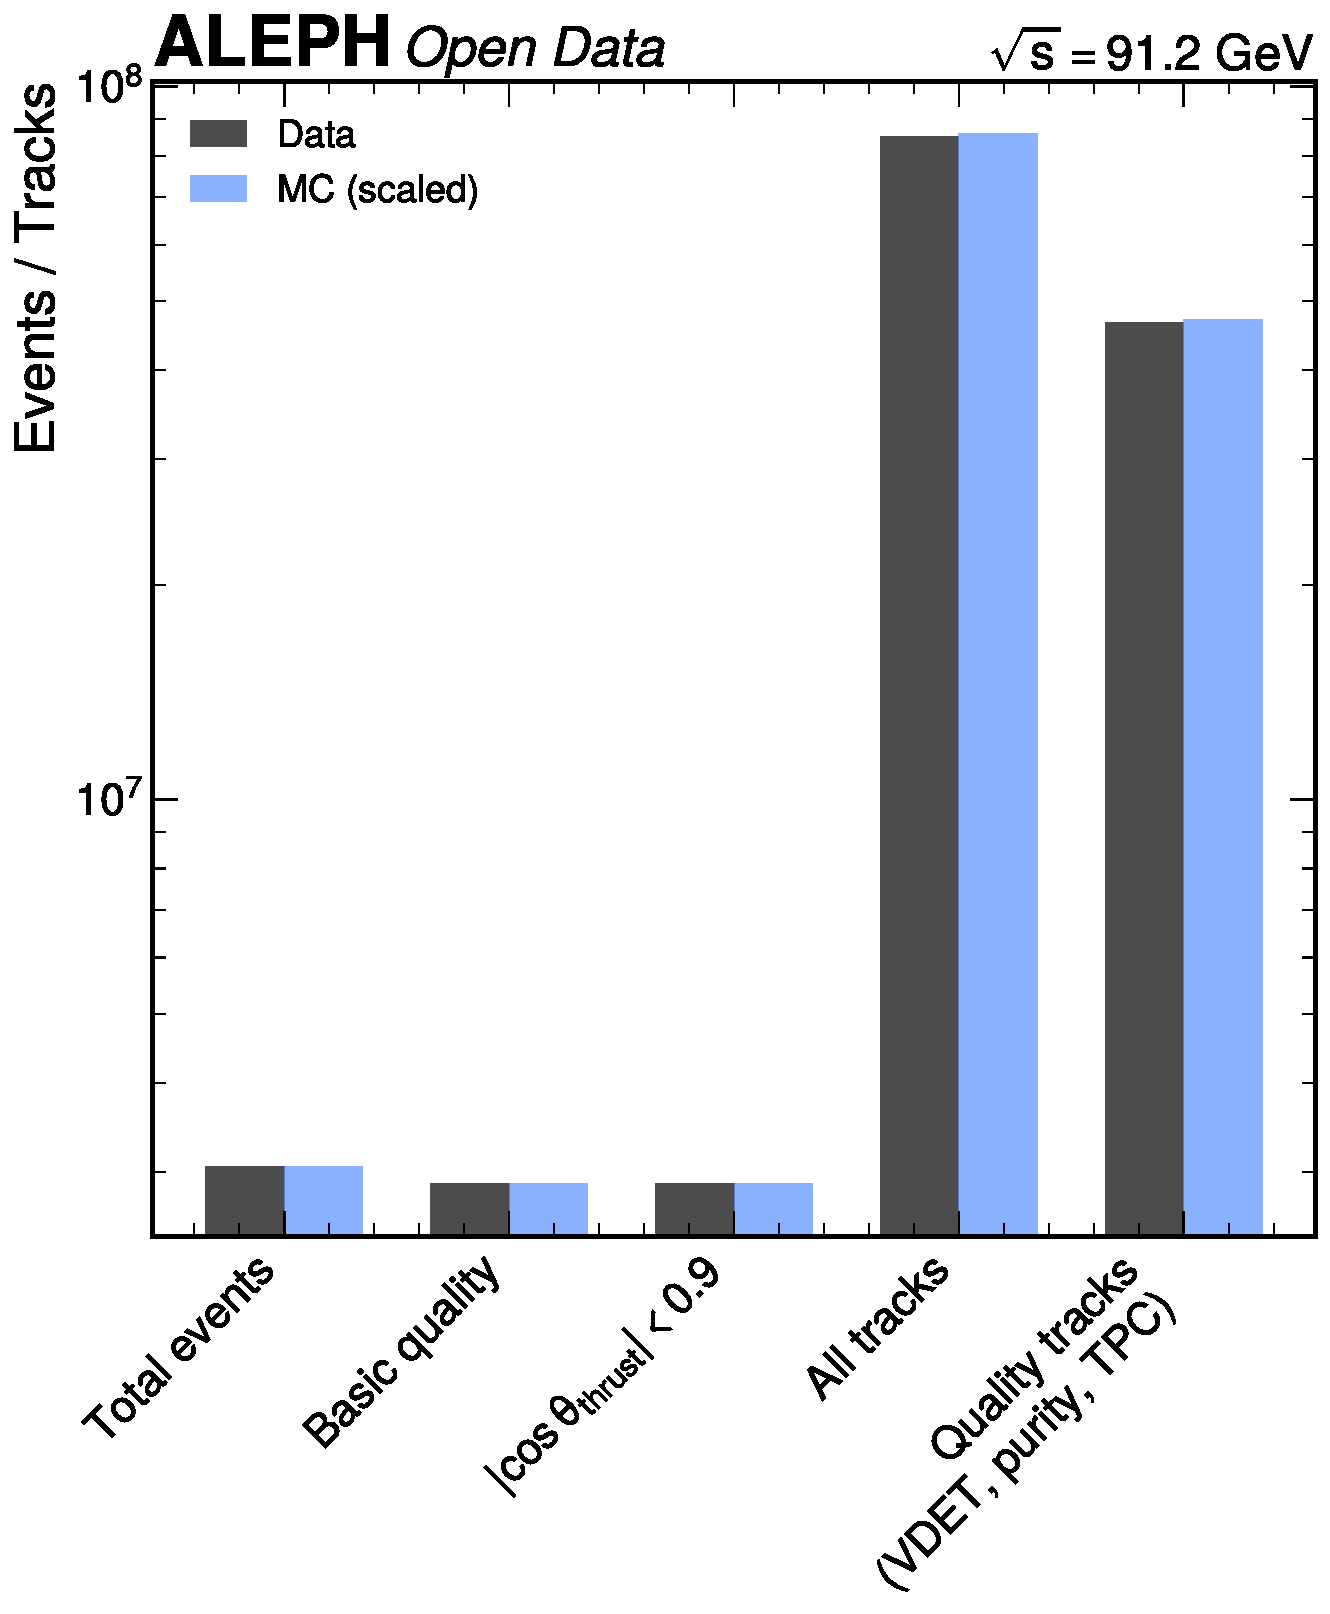
\includegraphics[height=0.45\linewidth]{figures/cutflow_magnus_1207_20260402.pdf}
\caption{Cutflow for data (black) and MC (red), showing the number of events
passing each successive selection requirement. The event-level preselection
retains 94.7\% of data events. The angular acceptance cut at
$|\cos\theta_\mathrm{thrust}| < 0.9$ removes a negligible additional fraction,
confirming that the pre-selection already enforces a similar angular requirement.}
\label{fig:cutflow}
\end{figure}

\subsection{Track quality requirements}
\label{sec:track_quality}

Tracks used for lifetime-based $b$-tagging must satisfy:
\begin{itemize}
\item $n_\mathrm{VDET} > 0$: at least one hit in the silicon vertex detector (VDET),
ensuring the track has a meaningful impact parameter measurement.
\item \texttt{highPurity} = 1: high-purity track reconstruction flag.
\item $n_\mathrm{TPC} > 4$: at least 5 hits in the time projection chamber (TPC),
ensuring good momentum resolution.
\end{itemize}

These requirements retain 54.9\% of data tracks (46.7~million out of 85.2~million).
The $\sim 45\%$ track loss is dominated by the $n_\mathrm{VDET} > 0$ requirement,
which removes the $\sim 36\%$ of tracks with sentinel $d_0 = -999$ values (tracks
without VDET hits). These tracks lack impact parameter information and cannot
contribute to lifetime tagging. However, they ARE included in the jet charge
computation (Section~\ref{sec:jetcharge}), which uses all charged tracks regardless
of VDET status.

\begin{table}[htbp]
\centering
\caption{Track selection cutflow. The VDET hit requirement dominates the track loss,
removing tracks without silicon vertex detector hits that cannot contribute to
lifetime-based $b$-tagging.}
\label{tab:track_cutflow}
\begin{tabular}{lrrr}
\toprule
Cut & Data tracks & MC tracks & Retention (data) \\
\midrule
All tracks & 85,198,110 & 21,700,304 & --- \\
Quality ($n_\mathrm{VDET} > 0$, HP, $n_\mathrm{TPC} > 4$) & 46,731,904 & 11,911,154 & 54.9\% \\
\bottomrule
\end{tabular}
\end{table}

\subsection{Data/MC comparison: event-level variables}
\label{sec:datamc_event}

Data/MC comparisons are produced for all variables entering the observable calculation.
The MC is normalized to the data integral in all plots. Agreement is generally good,
with no systematic trends in the pull distributions.

\begin{figure}[htbp]
\centering
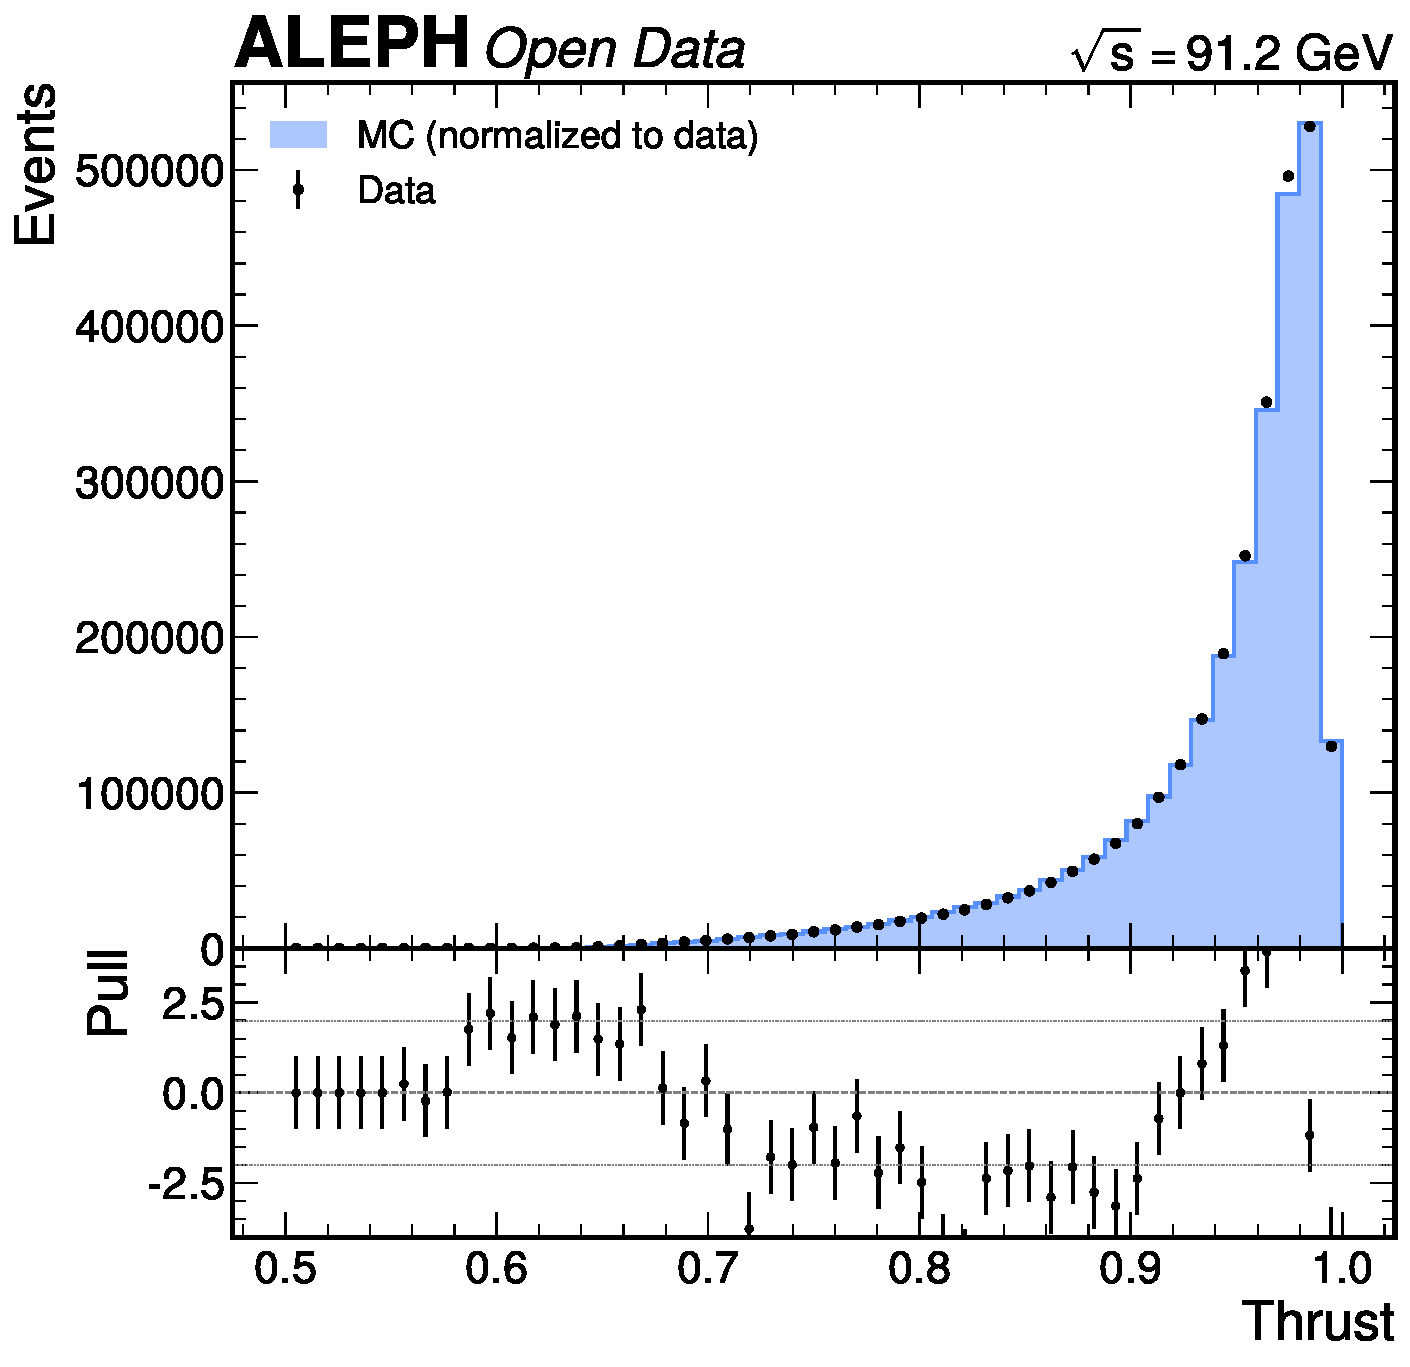
\includegraphics[height=0.32\linewidth]{figures/data_mc_thrust_magnus_1207_20260402.pdf}\hspace{1em}%
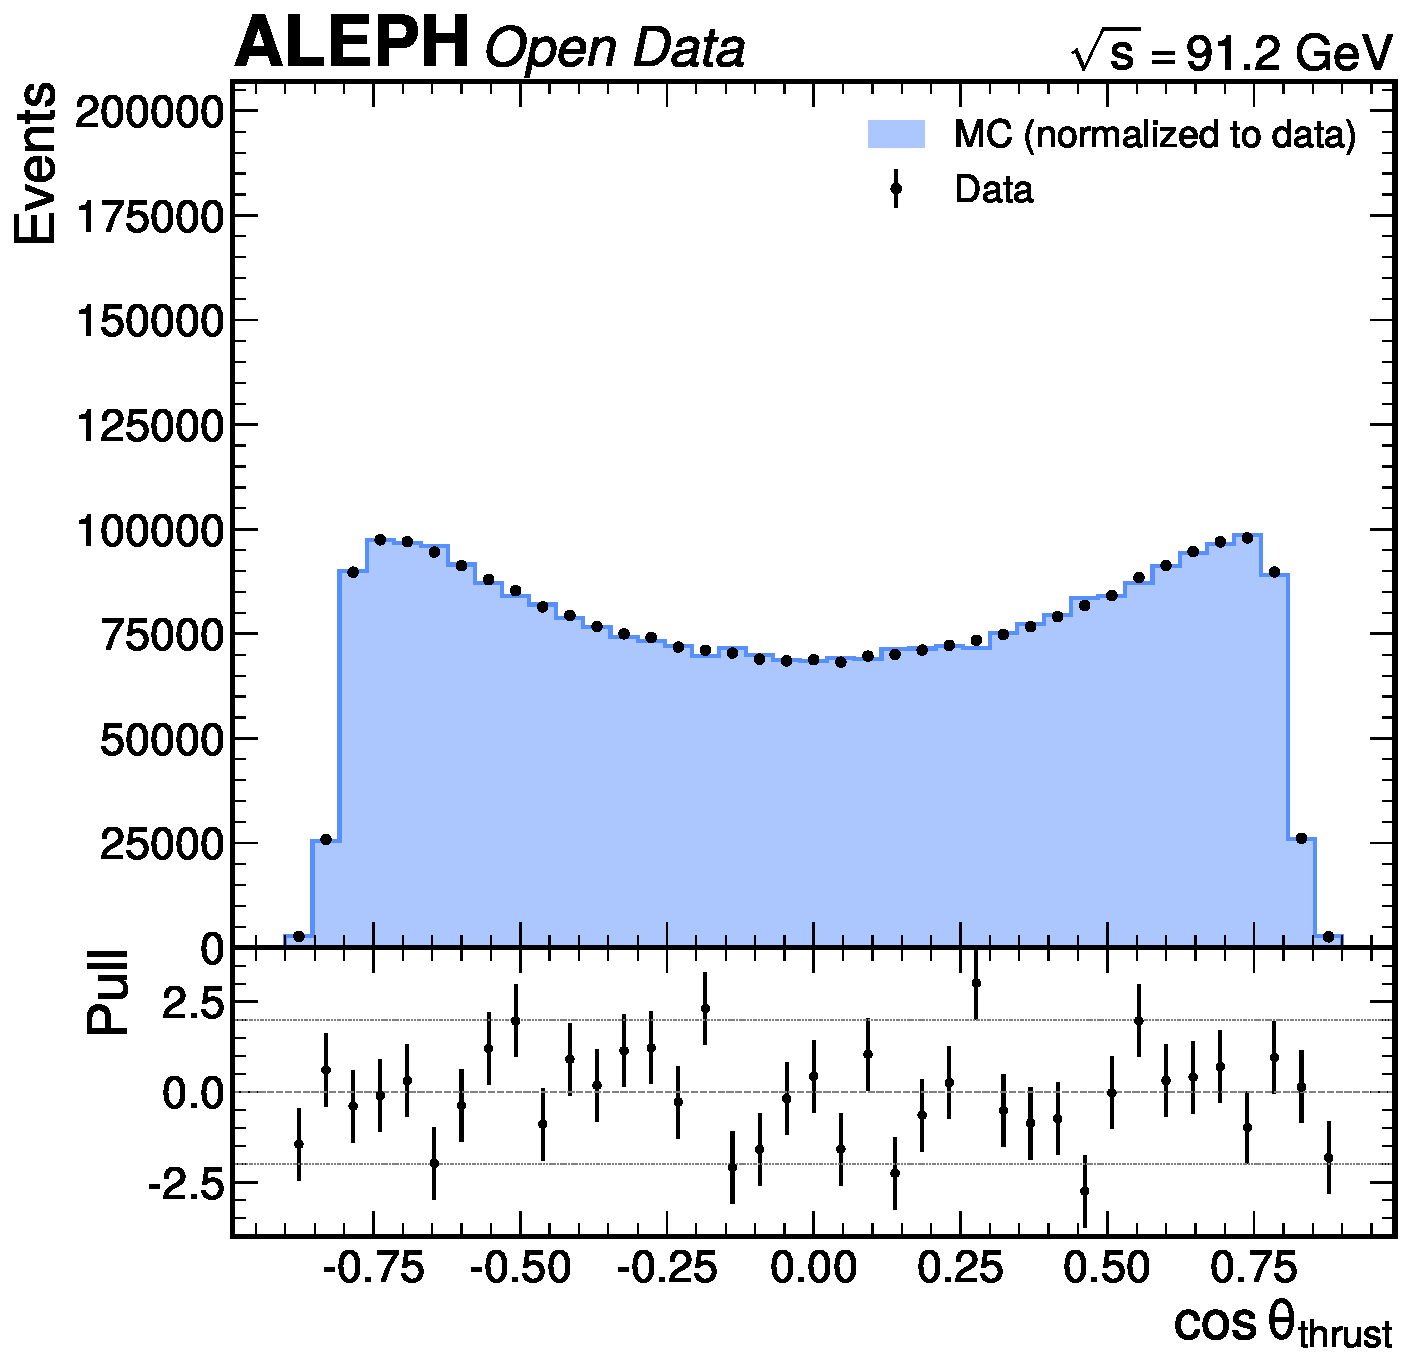
\includegraphics[height=0.32\linewidth]{figures/data_mc_costheta_magnus_1207_20260402.pdf}\\[0.5em]
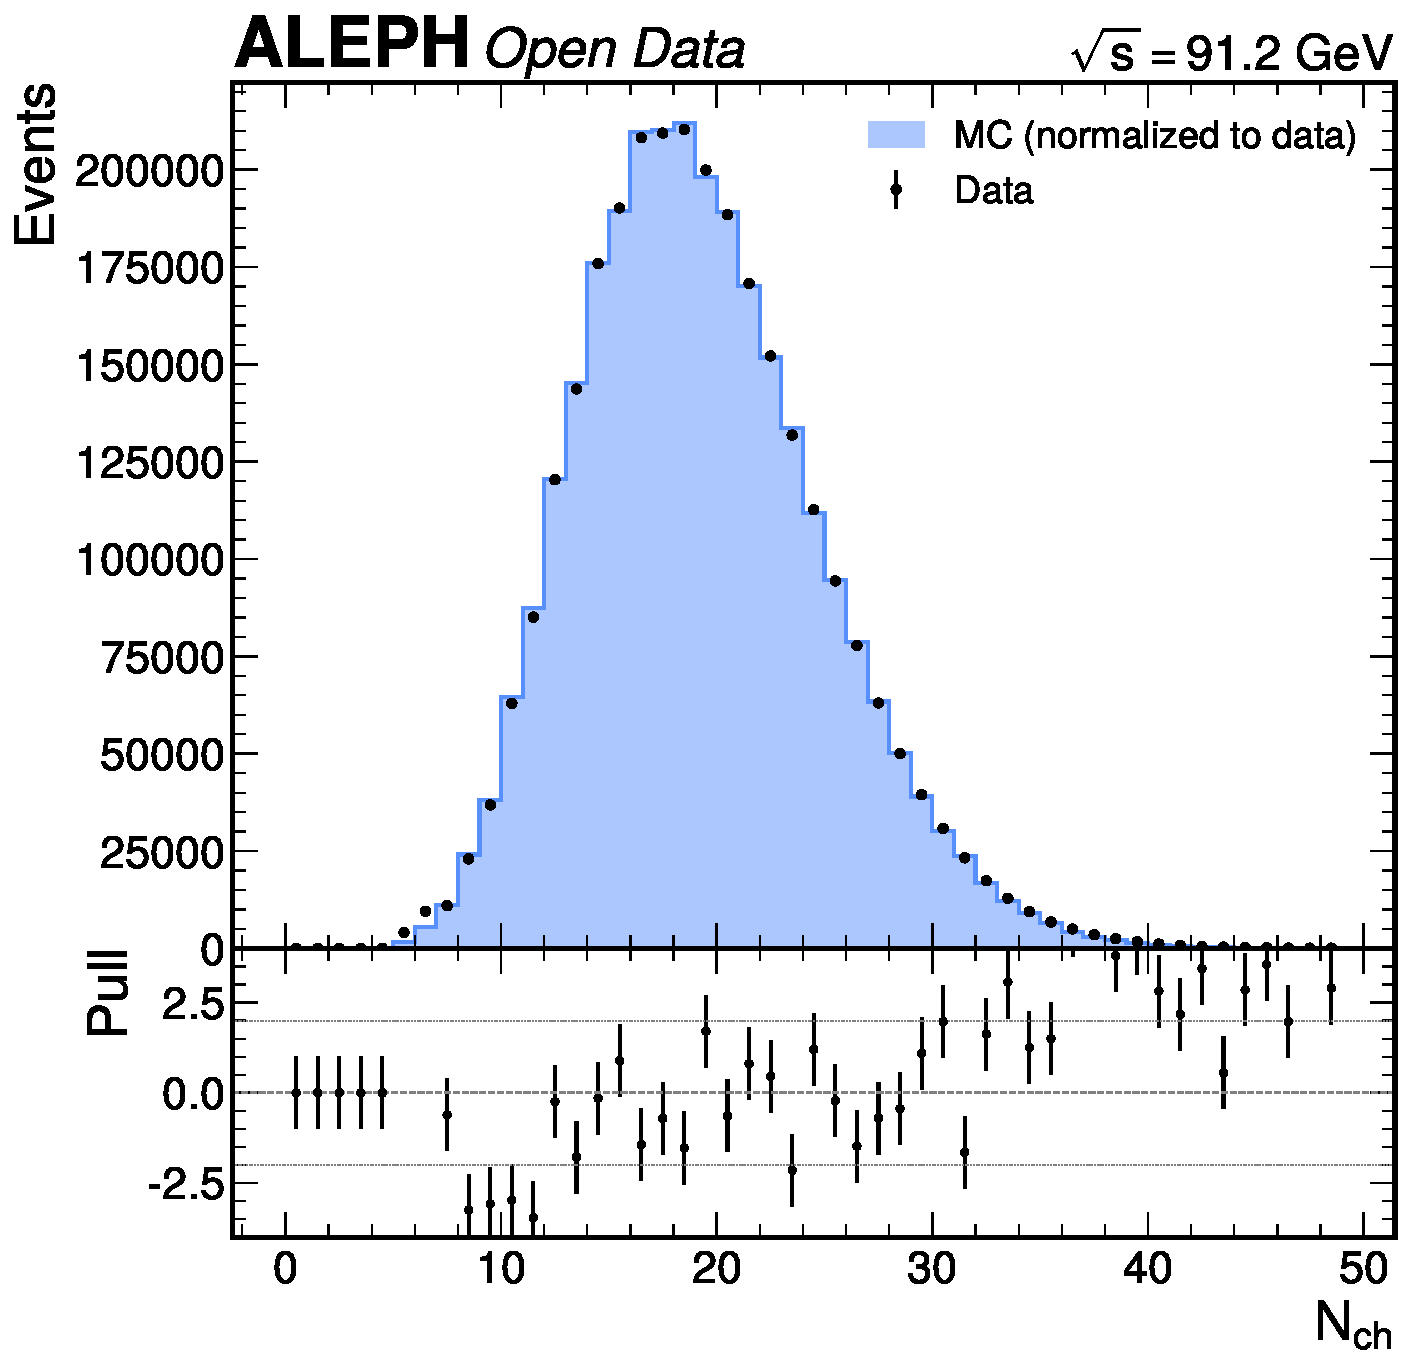
\includegraphics[height=0.32\linewidth]{figures/data_mc_nch_magnus_1207_20260402.pdf}\hspace{1em}%
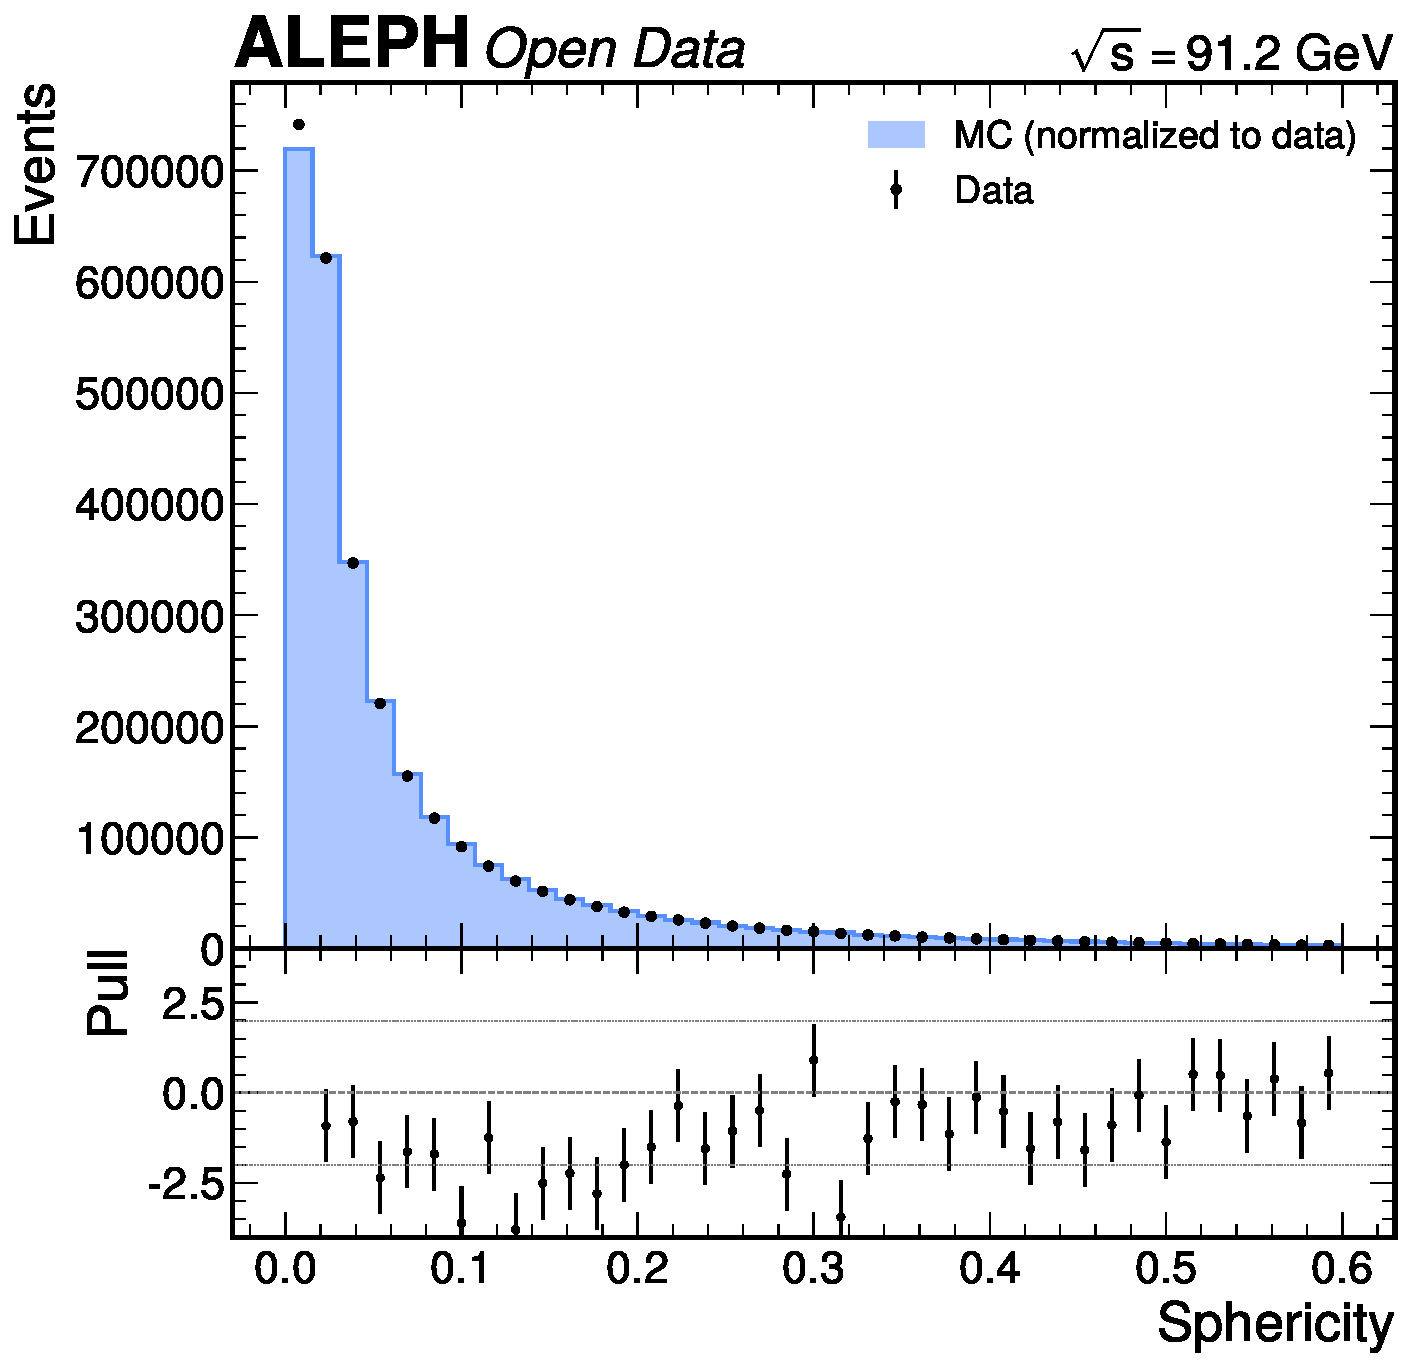
\includegraphics[height=0.32\linewidth]{figures/data_mc_sphericity_magnus_1207_20260402.pdf}
\caption{Data/MC comparisons for event-level variables after preselection:
thrust (top left), $\cos\theta_\mathrm{thrust}$ (top right), charged multiplicity
(bottom left), and sphericity (bottom right). The MC (1994 only) is normalized to
the data integral. Agreement is within 5\% across all variables, validating the MC
modelling of the event topology. The $\cos\theta_\mathrm{thrust}$ distribution shows
the expected $1 + \cos^2\theta$ shape, confirming the beam direction is correctly
encoded in the coordinate system.}
\label{fig:datamc_event}
\end{figure}

\begin{figure}[htbp]
\centering
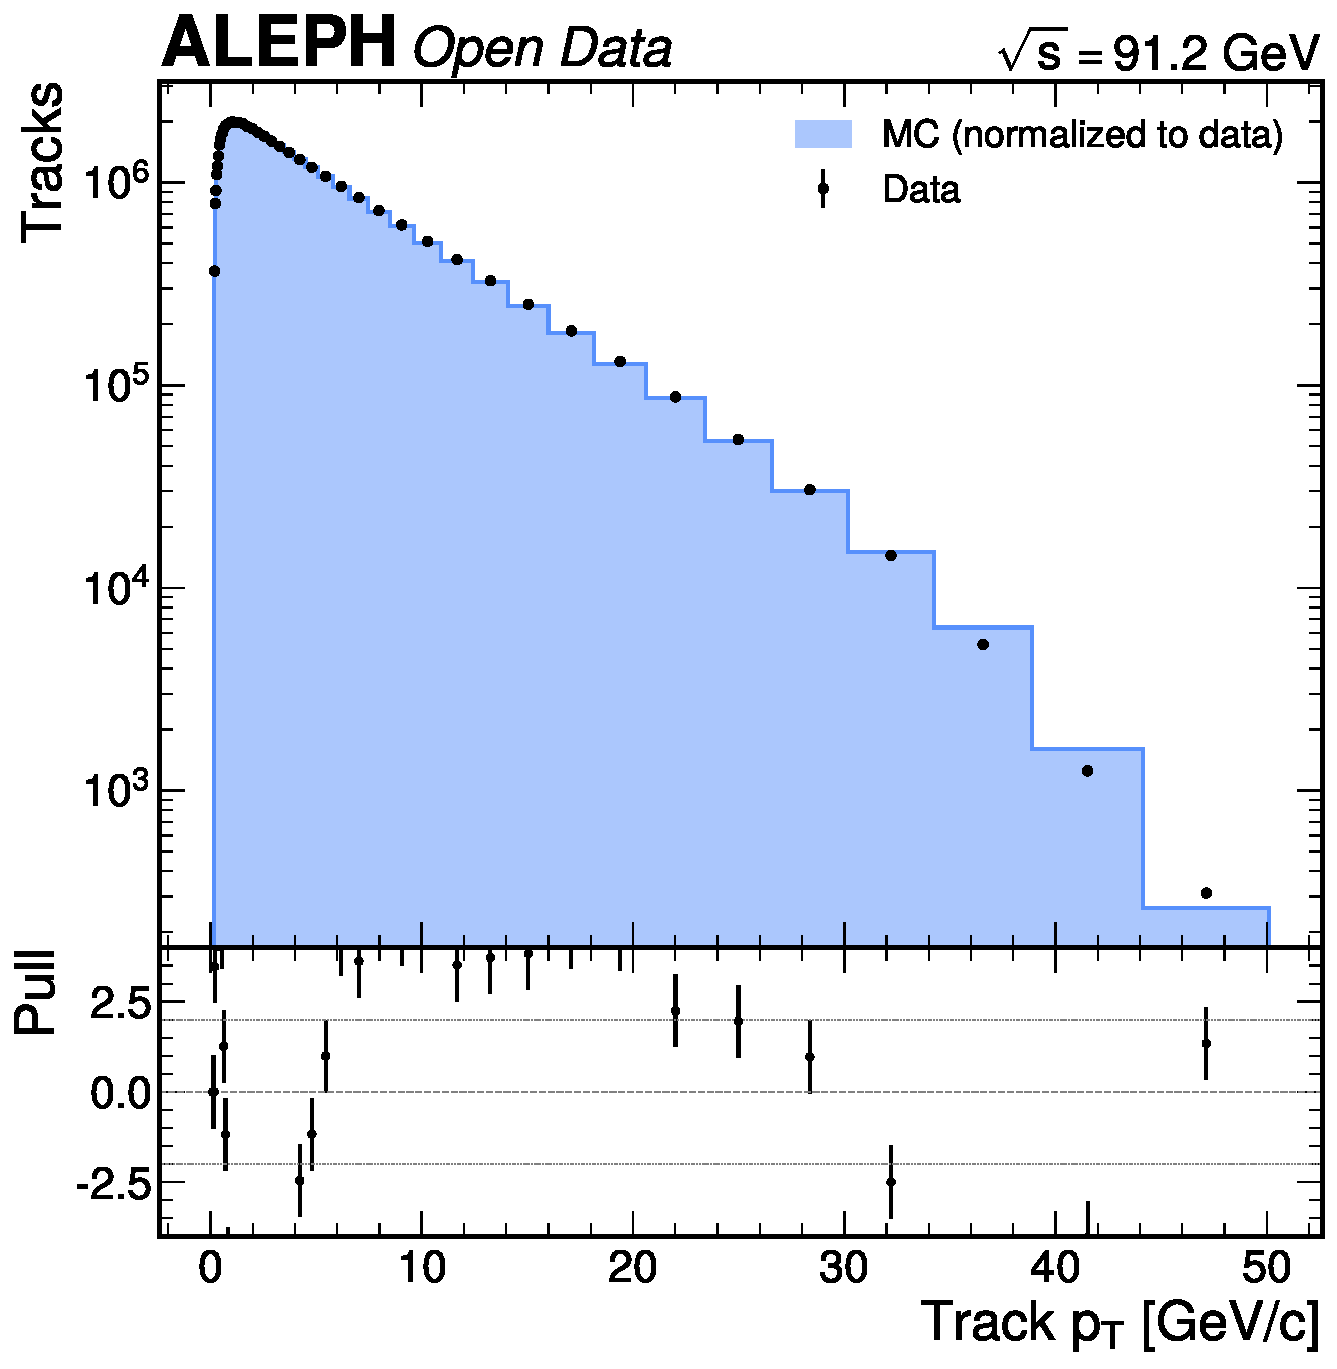
\includegraphics[height=0.38\linewidth]{figures/data_mc_trackpt_magnus_1207_20260402.pdf}\hspace{1em}%
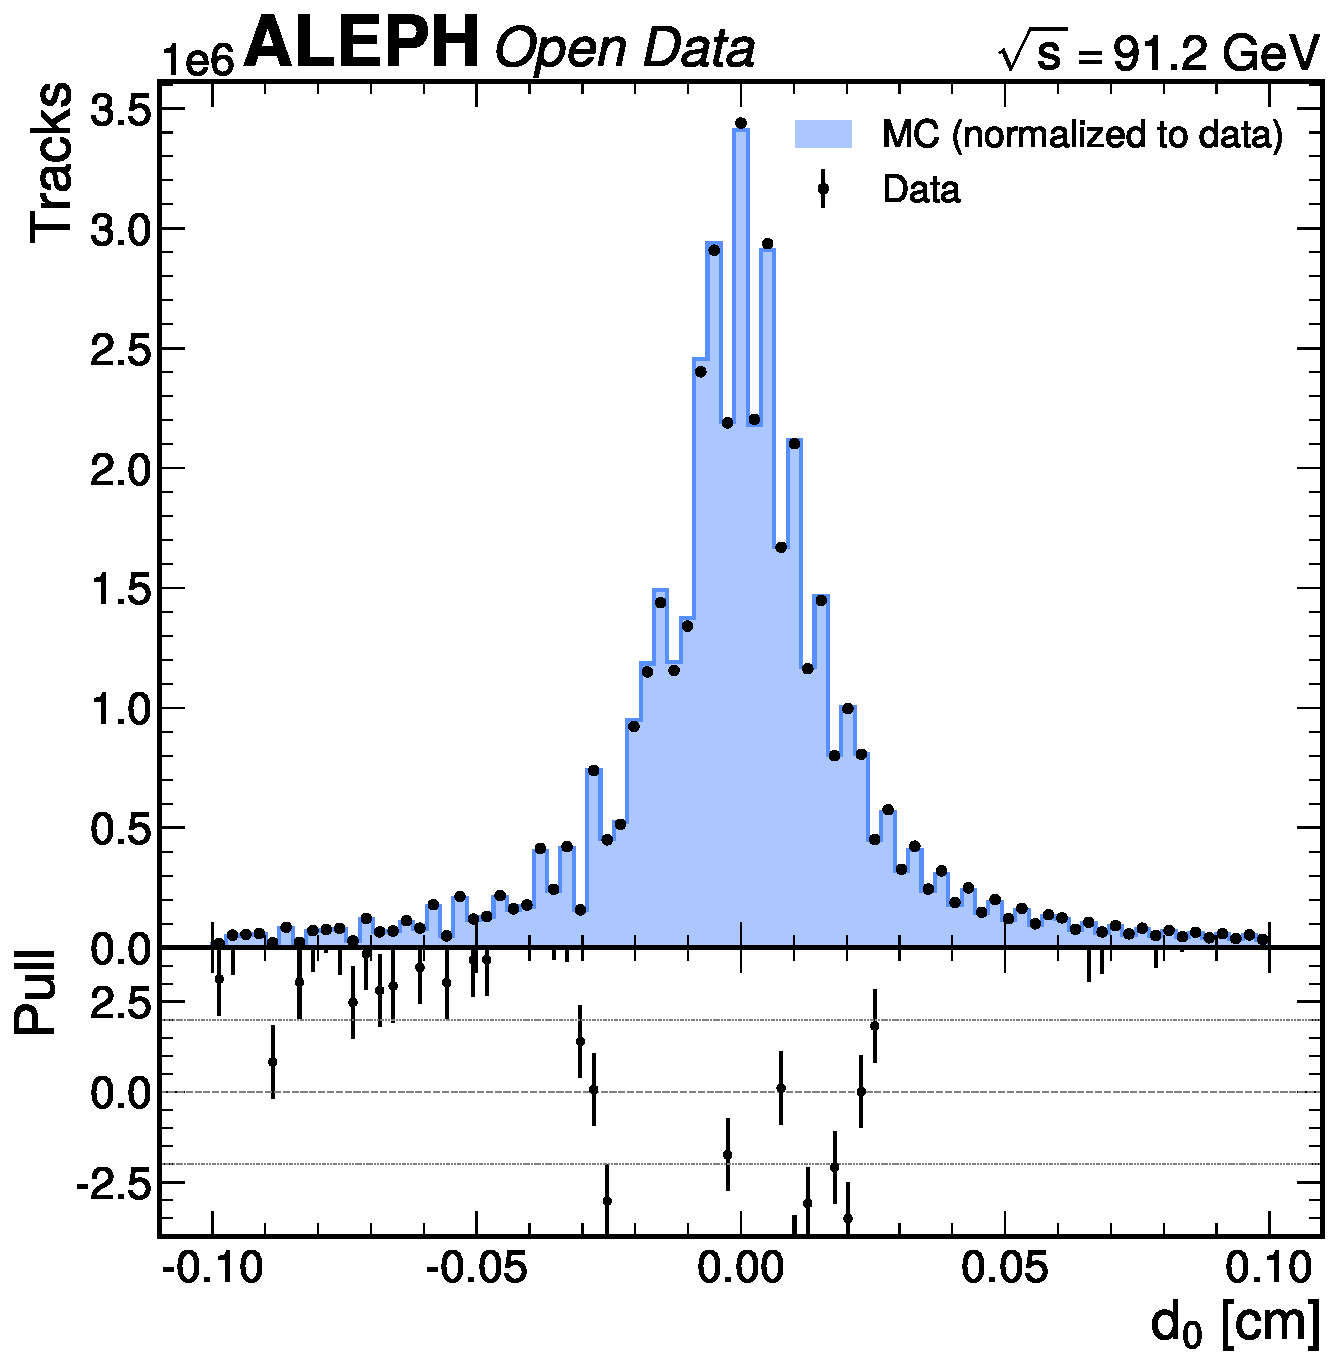
\includegraphics[height=0.38\linewidth]{figures/data_mc_d0_magnus_1207_20260402.pdf}
\caption{Data/MC comparisons for track-level variables: track $p_T$ (left) and
impact parameter $d_0$ (right). The track $p_T$ distribution shows good agreement
over three orders of magnitude. The $d_0$ distribution agrees well in the core
(resolution-dominated region); the extended tails from heavy-flavour decays show
some data-MC discrepancy, consistent with the known 10\% resolution difference
(data has worse effective resolution than MC due to beam spot and vertex effects).}
\label{fig:datamc_track}
\end{figure}

% --- Additional Phase 1 data/MC figures ---
\subsection{Data/MC comparison: Phase 1 exploration}
\label{sec:datamc_phase1}

The Phase~1 data reconnaissance produced data/MC comparisons on a 5000-event survey
across a comprehensive set of kinematic variables. These plots confirmed the basic
data quality and MC modelling before the full analysis chain was constructed.
Figures~\ref{fig:p1_thrust_costheta} and~\ref{fig:p1_nch_sphericity} show the
Phase~1 versions of the key event-level variables.

\begin{figure}[htbp]
\centering
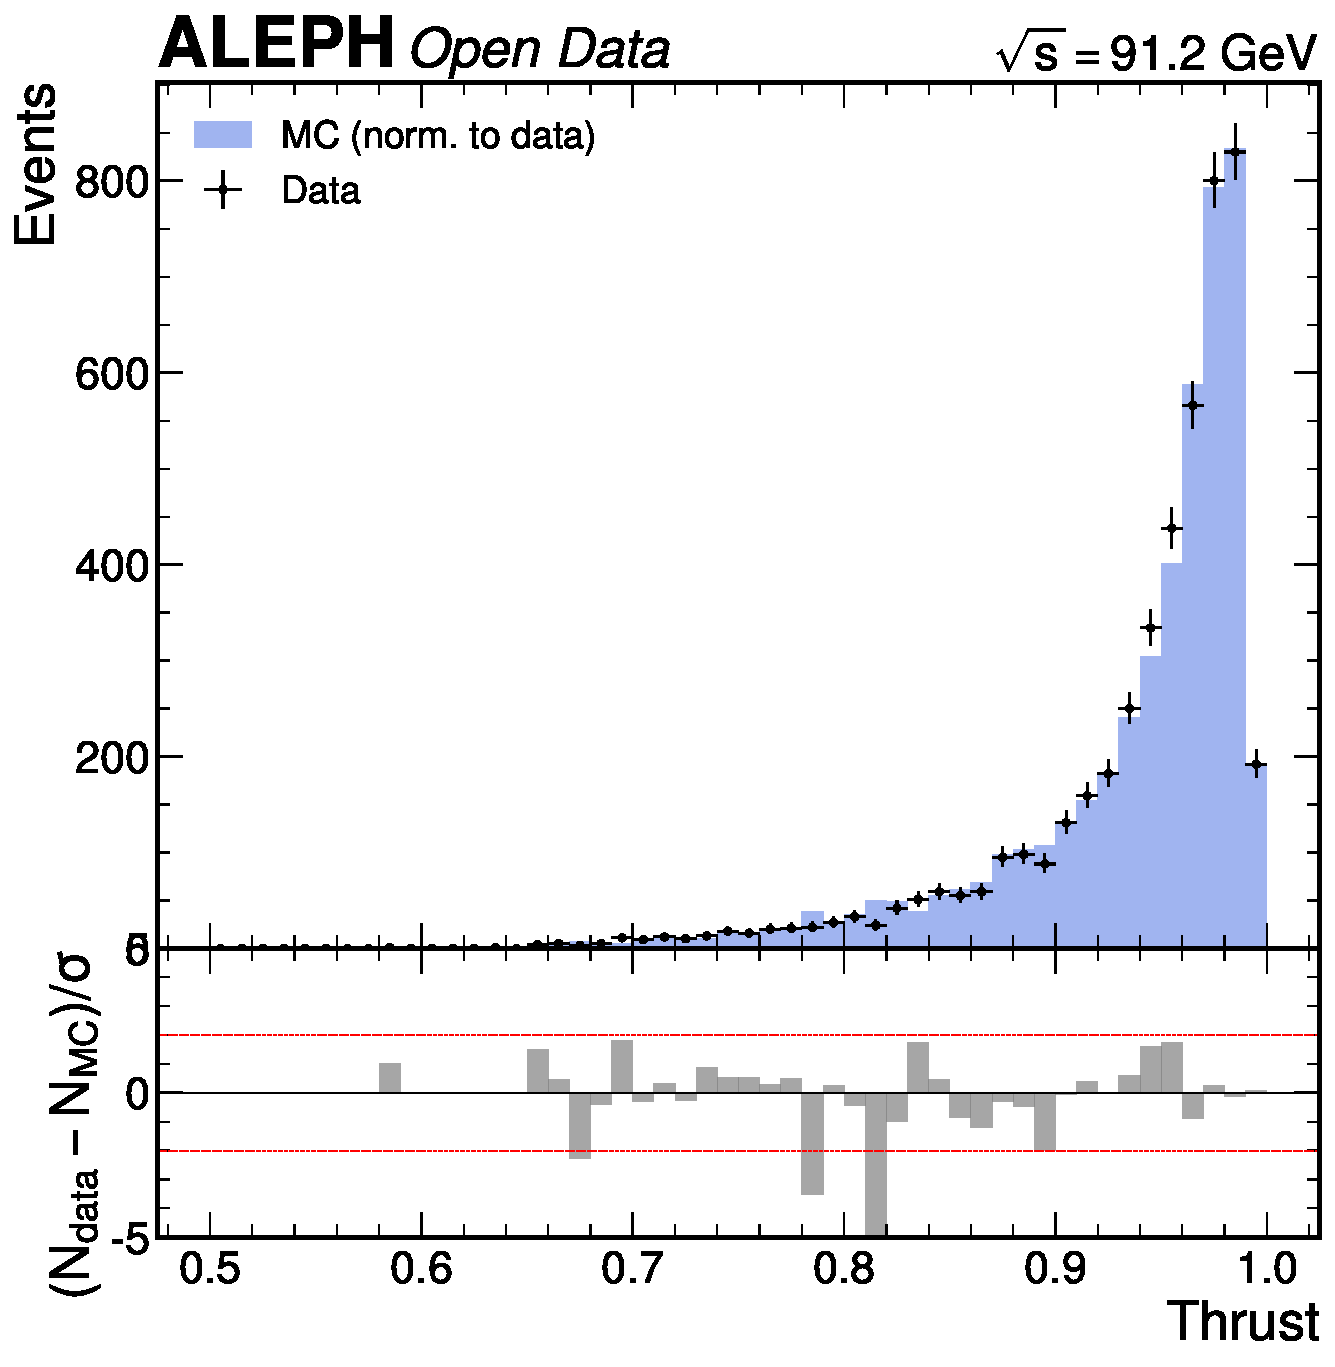
\includegraphics[height=0.38\linewidth]{figures/data_mc_thrust_fabiola_b942.pdf}\hspace{1em}%
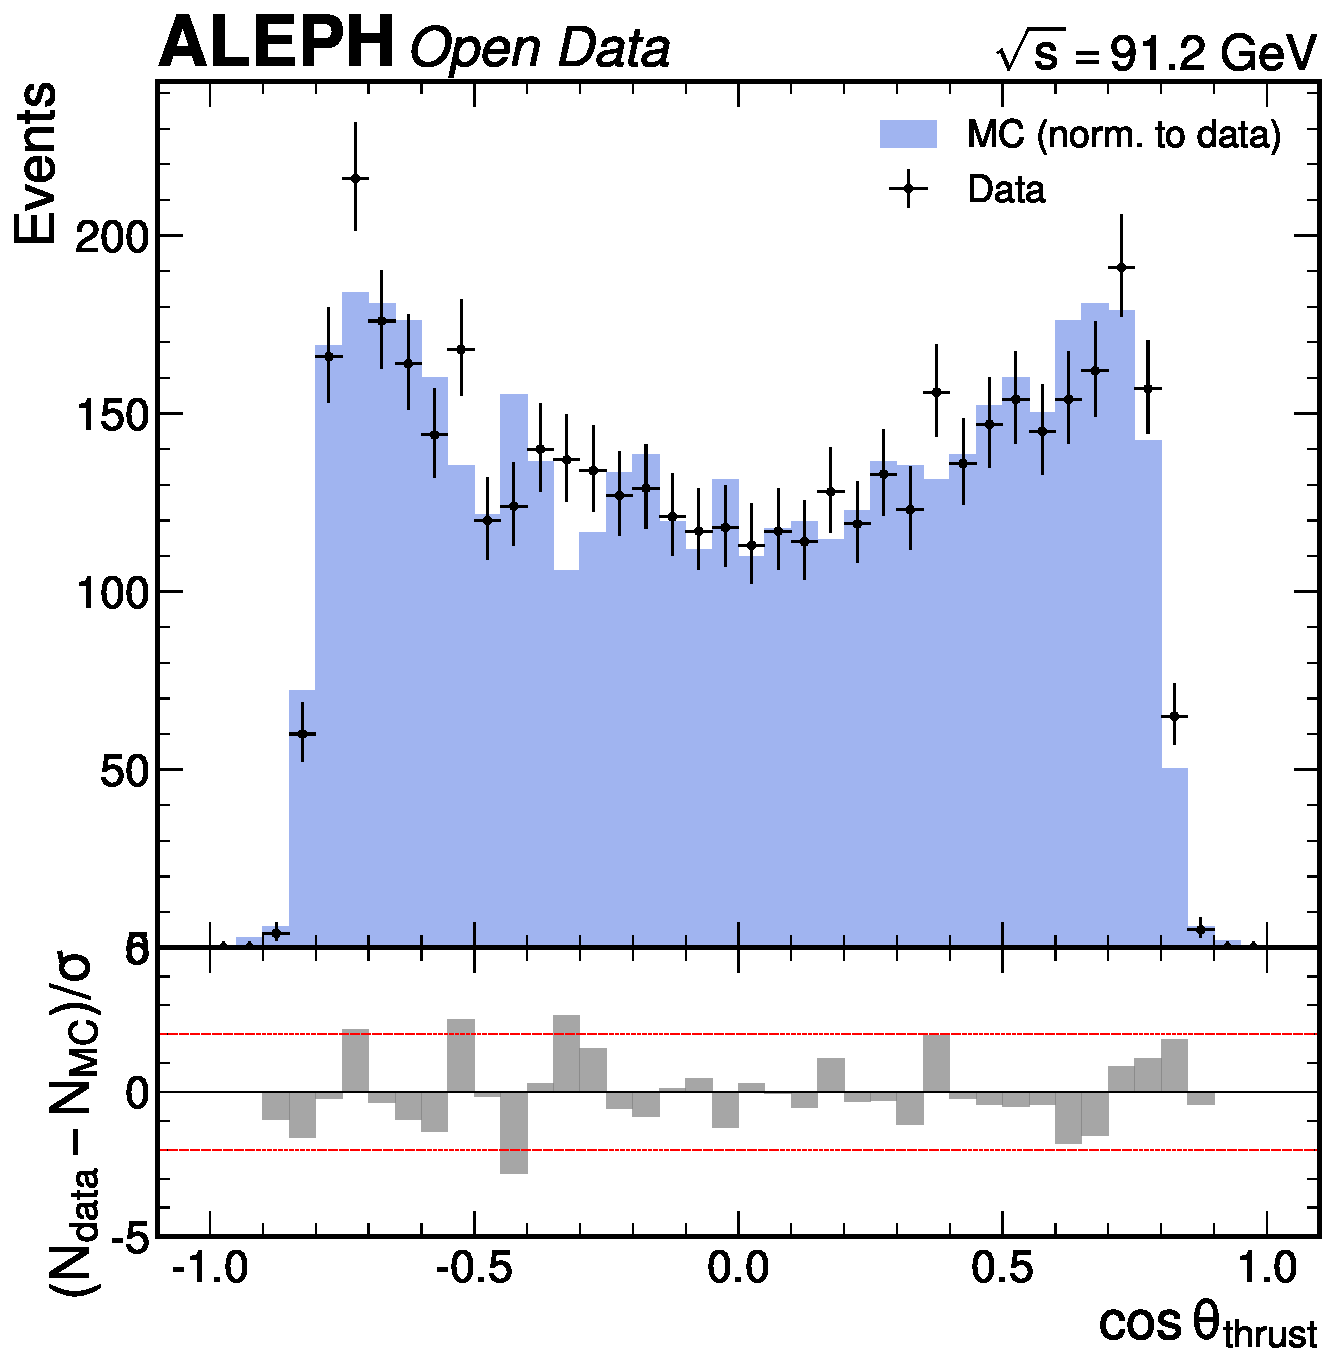
\includegraphics[height=0.38\linewidth]{figures/data_mc_costheta_fabiola_b942.pdf}
\caption{Phase~1 data/MC comparisons for thrust (left) and $\cos\theta_\mathrm{thrust}$
(right) from the initial 5000-event survey. These early comparisons confirmed that the
MC modelling of event topology was adequate before committing to the full analysis chain.
The thrust distribution peaks near 0.9, characteristic of two-jet events at the $Z$ pole.
The $\cos\theta_\mathrm{thrust}$ distribution shows the expected $1 + \cos^2\theta$ shape
from the electroweak $Z \to q\bar{q}$ production.}
\label{fig:p1_thrust_costheta}
\end{figure}

\begin{figure}[htbp]
\centering
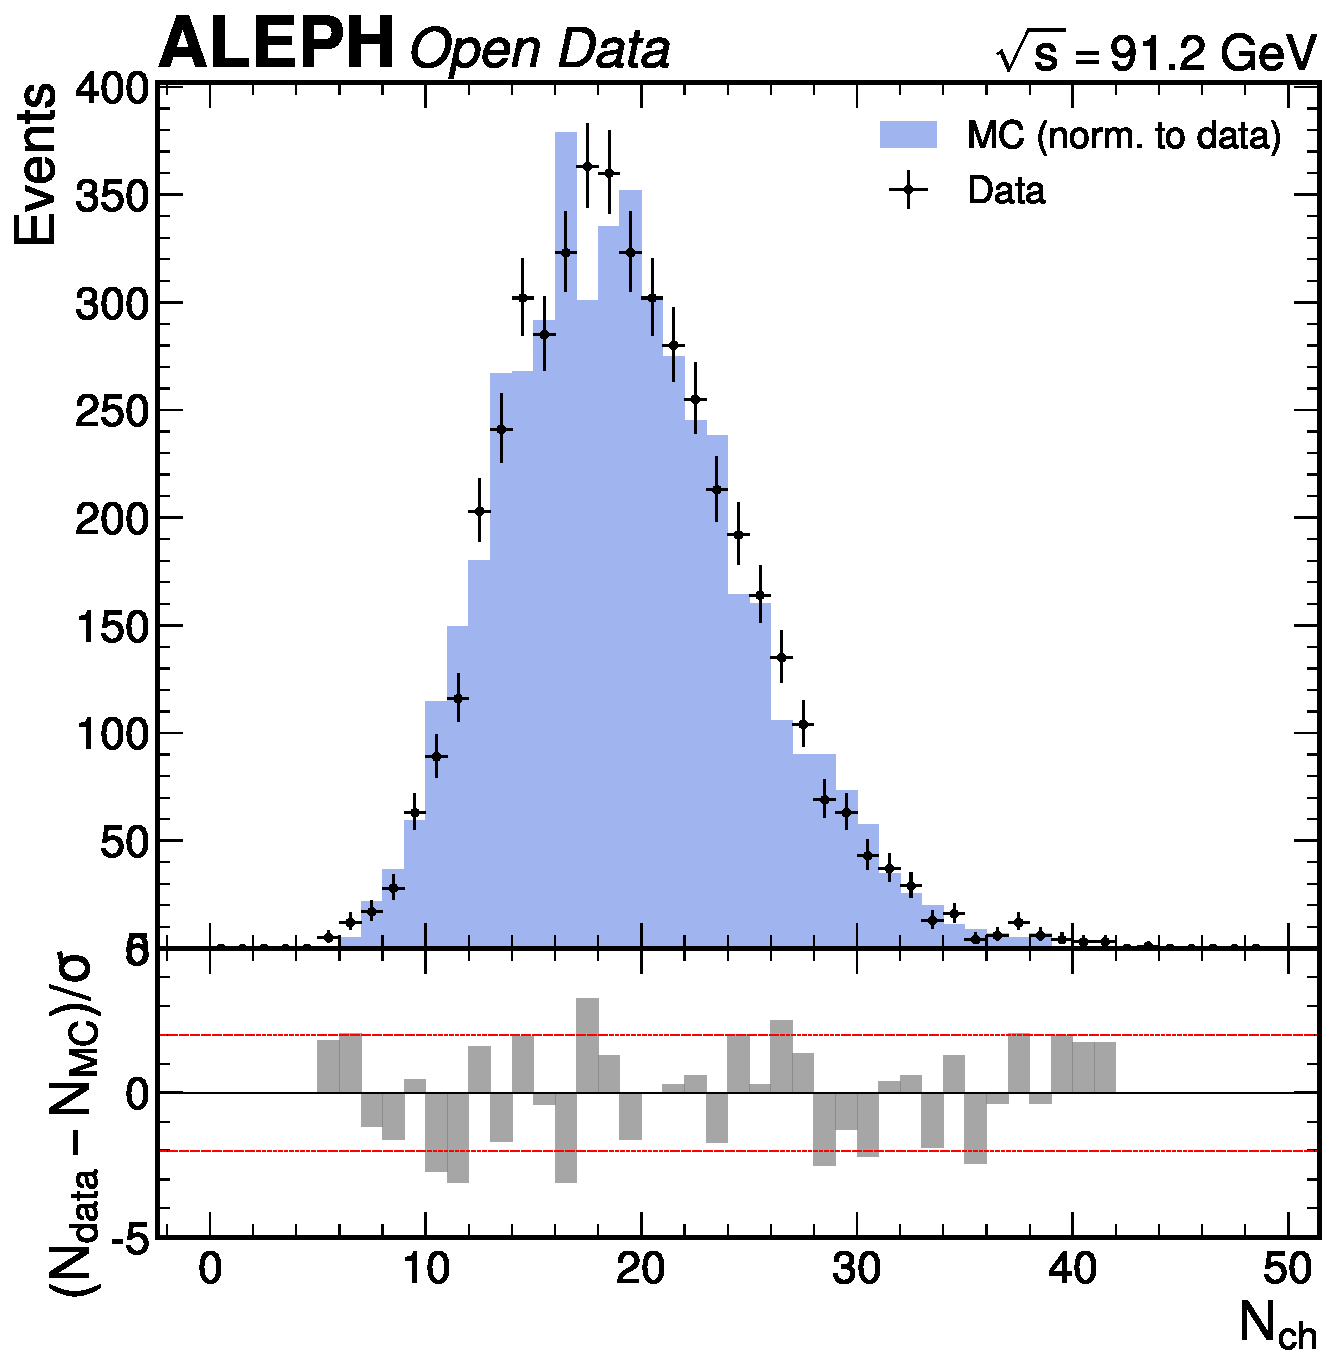
\includegraphics[height=0.38\linewidth]{figures/data_mc_nch_fabiola_b942.pdf}\hspace{1em}%
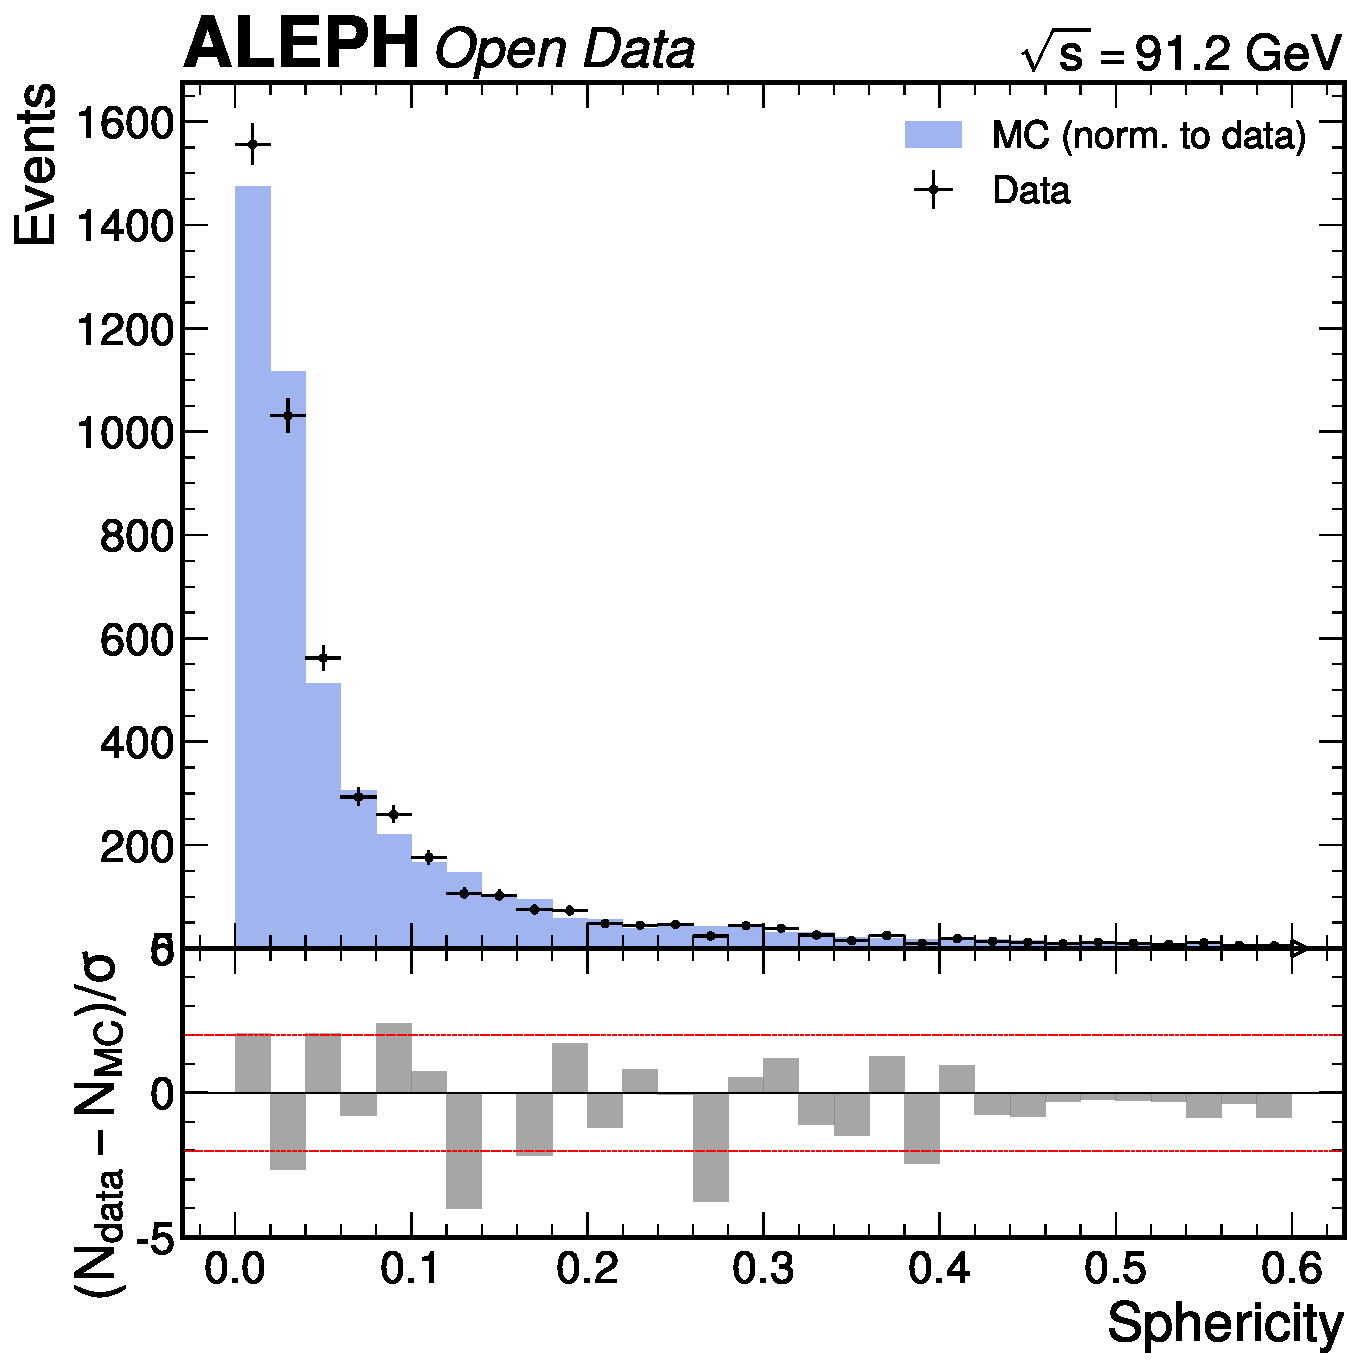
\includegraphics[height=0.38\linewidth]{figures/data_mc_sphericity_fabiola_b942.pdf}
\caption{Phase~1 data/MC comparisons for charged multiplicity (left) and sphericity
(right). The charged multiplicity distribution has a mean of approximately 19 tracks per
event, with data and MC showing good agreement. The sphericity distribution peaks at low
values (pencil-like events from two-jet topology) with a tail toward higher values from
multi-jet events. Both variables were validated as inputs to the analysis strategy.}
\label{fig:p1_nch_sphericity}
\end{figure}

\begin{figure}[htbp]
\centering
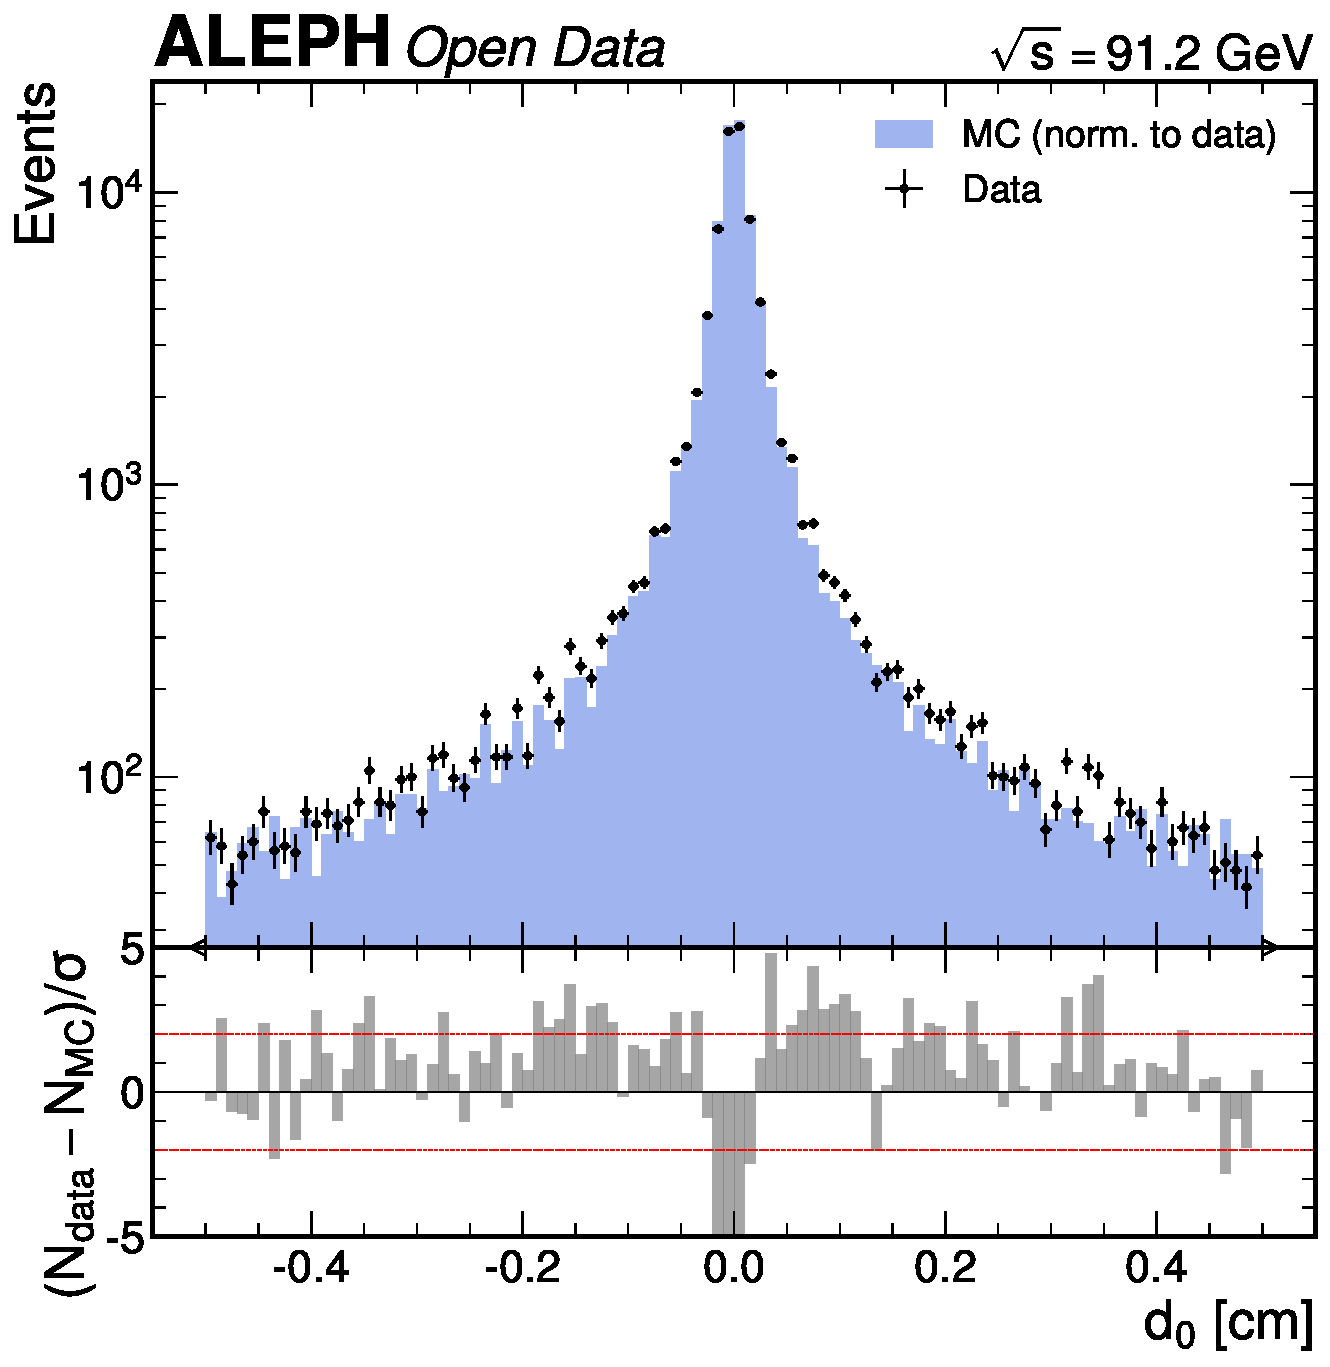
\includegraphics[height=0.38\linewidth]{figures/data_mc_d0_fabiola_b942.pdf}\hspace{1em}%
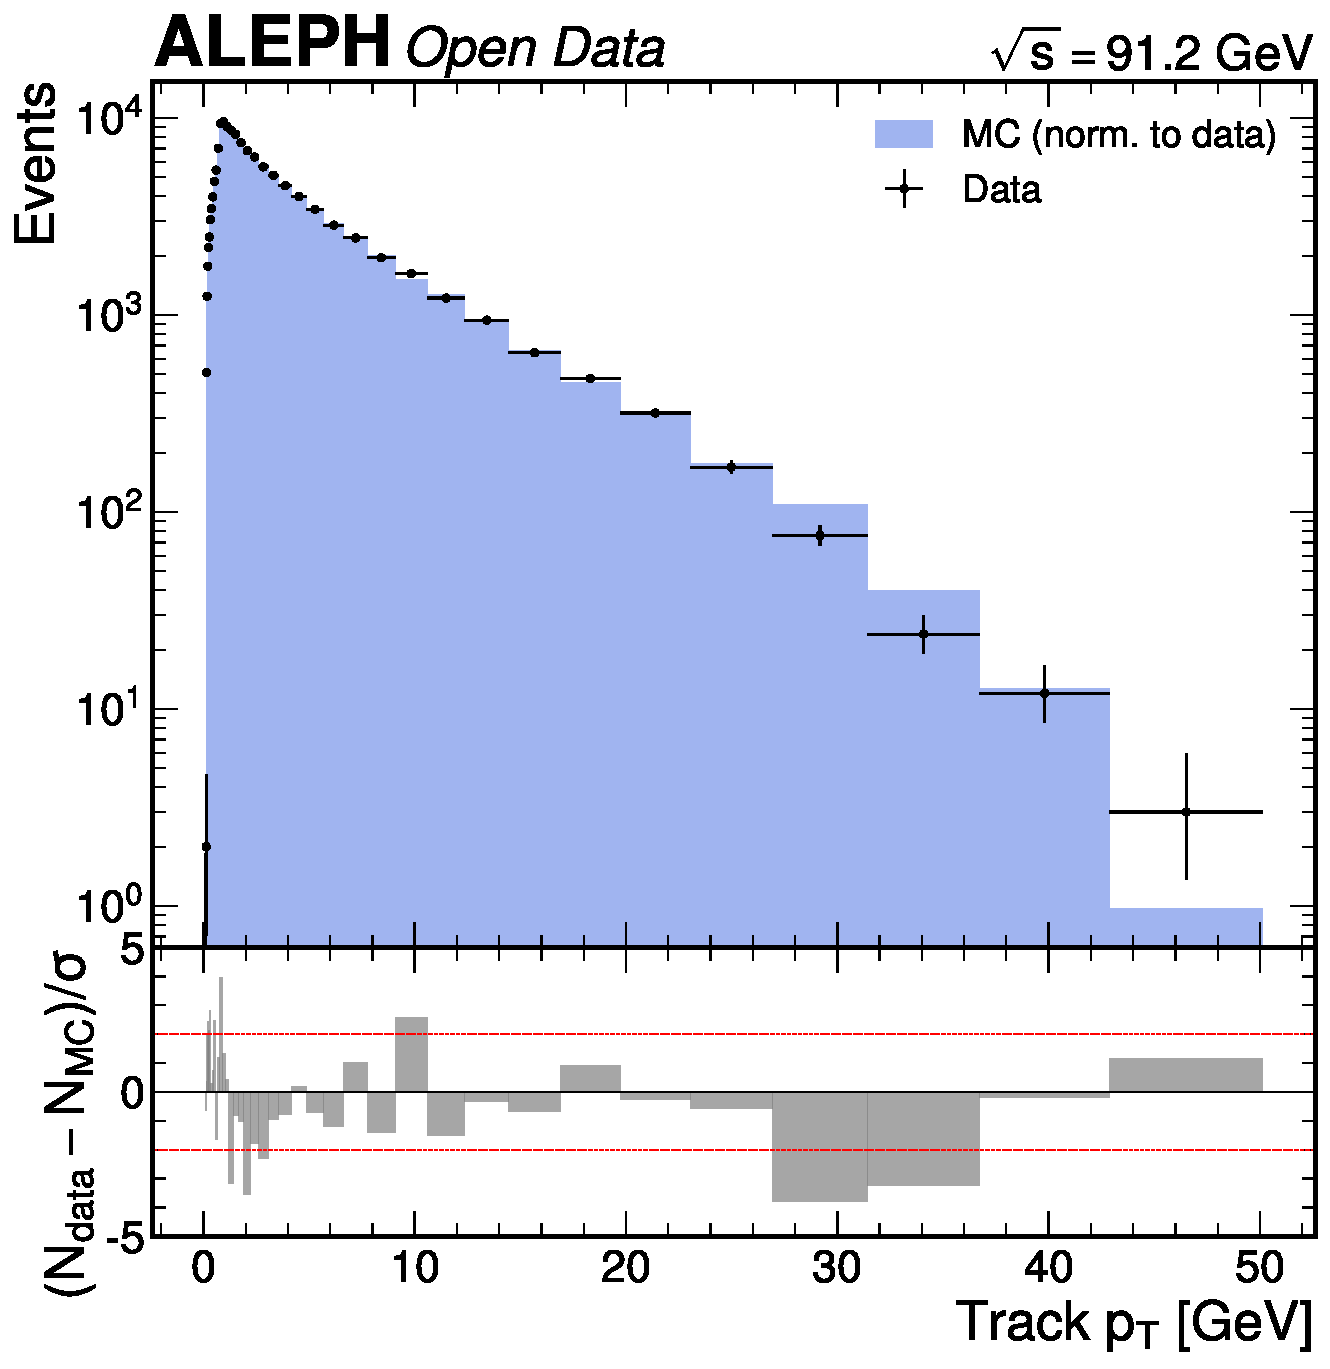
\includegraphics[height=0.38\linewidth]{figures/data_mc_trackpt_fabiola_b942.pdf}
\caption{Phase~1 data/MC comparisons for the transverse impact parameter $d_0$ (left) and
track $p_T$ (right). The $d_0$ distribution is resolution-dominated in the core with
extended tails from heavy-flavour decays. The track $p_T$ distribution spans three orders
of magnitude with good data/MC agreement. The extended positive $d_0$ tail visible in
this plot is the key feature exploited by the lifetime-based $b$-tag.}
\label{fig:p1_d0_trackpt}
\end{figure}

\subsection{Selection approach comparison}
\label{sec:selection_comparison}

Two hemisphere tagging approaches were implemented and compared, as required by the
analysis strategy:

\begin{enumerate}
\item \textbf{Combined probability-mass tag (primary):} Uses the per-hemisphere probability
product from signed impact parameter significances, combined with a displaced-track
invariant mass component. This provides a continuous discriminant with fine working-point
control (Section~\ref{sec:prob_tag}).

\item \textbf{$N$-sigma counting tag (cross-check):} Counts tracks with signed significance
above a threshold $N_\mathrm{cut}$. Simpler but less powerful, lacking the probability
and mass information.
\end{enumerate}

The comparison at matched single-tag fractions shows:
\begin{itemize}
\item At $f_s \approx 0.06$: the $N$-sigma tag ($N_\mathrm{cut} = 3$) gives $f_d = 0.009$,
while the combined tag (WP $\approx 12$) gives $f_d \approx 0.020$ --- approximately
$2\times$ higher double-tag efficiency at the same single-tag purity.
\item At $f_s \approx 0.17$: the combined tag (WP~10.0) gives $f_d = 0.044$, significantly
exceeding the $N$-sigma tag at comparable purity.
\end{itemize}

The combined tag is retained as primary due to its superior double-tag efficiency, which
directly translates to smaller statistical uncertainty on $R_b$. The $N$-sigma tag is
retained as a robustness cross-check.

A BDT-based tagger [D9, D10] was planned in the strategy but formally downscoped
because the \texttt{bFlag} branch (the only candidate for proxy labels) tags 99.8\%
of events after preselection, making it unsuitable as a $b$-enrichment label for training.
Self-labelling from the cut-based tag remains viable and will be attempted in Phase~4b/4c.

% =====================================================================
% 4. CORRECTIONS
% =====================================================================
\FloatBarrier
\needspace{4\baselineskip}
\section{Corrections}
\label{sec:corrections}

This section describes the correction chain from raw event counts to the final
physics observables. The double-tag method for $R_b$ is inherently self-correcting
for the $b$-tagging efficiency; the remaining corrections involve the impact parameter
resolution, hemisphere correlation, and background efficiencies.

\subsection{Impact parameter resolution ($\sigma_{d_0}$)}
\label{sec:sigma_d0}

The transverse impact parameter resolution $\sigma_{d_0}$ is parameterized as:
\begin{equation}
\sigma_{d_0} = \sqrt{A^2 + \left(\frac{B}{p \sin\theta}\right)^2},
\label{eq:sigma_d0}
\end{equation}
where $A = 25\;\mu\mathrm{m}$ is the intrinsic VDET resolution and
$B = 70\;\mu\mathrm{m}\cdot\mathrm{GeV}/c$ is the multiple-scattering
term~\cite{ALEPH:VDET}. The $\sin\theta$ dependence (not $\sin^{3/2}\theta$)
is the correct form for the $R\phi$-projected impact parameter $d_0$; the
$\sin^{3/2}\theta$ form applies to 3D impact parameters.

The parameterization is calibrated using the negative $d_0/\sigma_{d_0}$ distribution,
which arises purely from resolution effects (no lifetime contribution). Tracks with
genuinely negative signed impact parameters (upstream of the primary vertex along the
jet direction) provide a clean resolution sample. The calibration is performed in
40 bins: 5 momentum bins $\times$ 4 $|\cos\theta|$ bins $\times$ 2 $n_\mathrm{VDET}$
classes (1 hit, $\geq 2$ hits). Each bin must contain $> 1000$ negative-$d_0$ tracks.

The calibrated scale factors range from 1.3 to 7.6 across the 40 bins. Tracks with
$\geq 2$ VDET hits have smaller scale factors (1.3--2.7) than 1-VDET tracks (2.5--7.6),
reflecting the better resolution with more silicon layers. The scale factors indicate
that the nominal $A$, $B$ parameters underestimate the actual resolution by factors
of 1.3--7.6$\times$, attributable to beam spot size, primary vertex uncertainty, and
detector alignment effects not captured by the simple two-parameter model.

Figure~\ref{fig:sigma_d0_calibration} shows the calibration scale factors.

\begin{figure}[htbp]
\centering
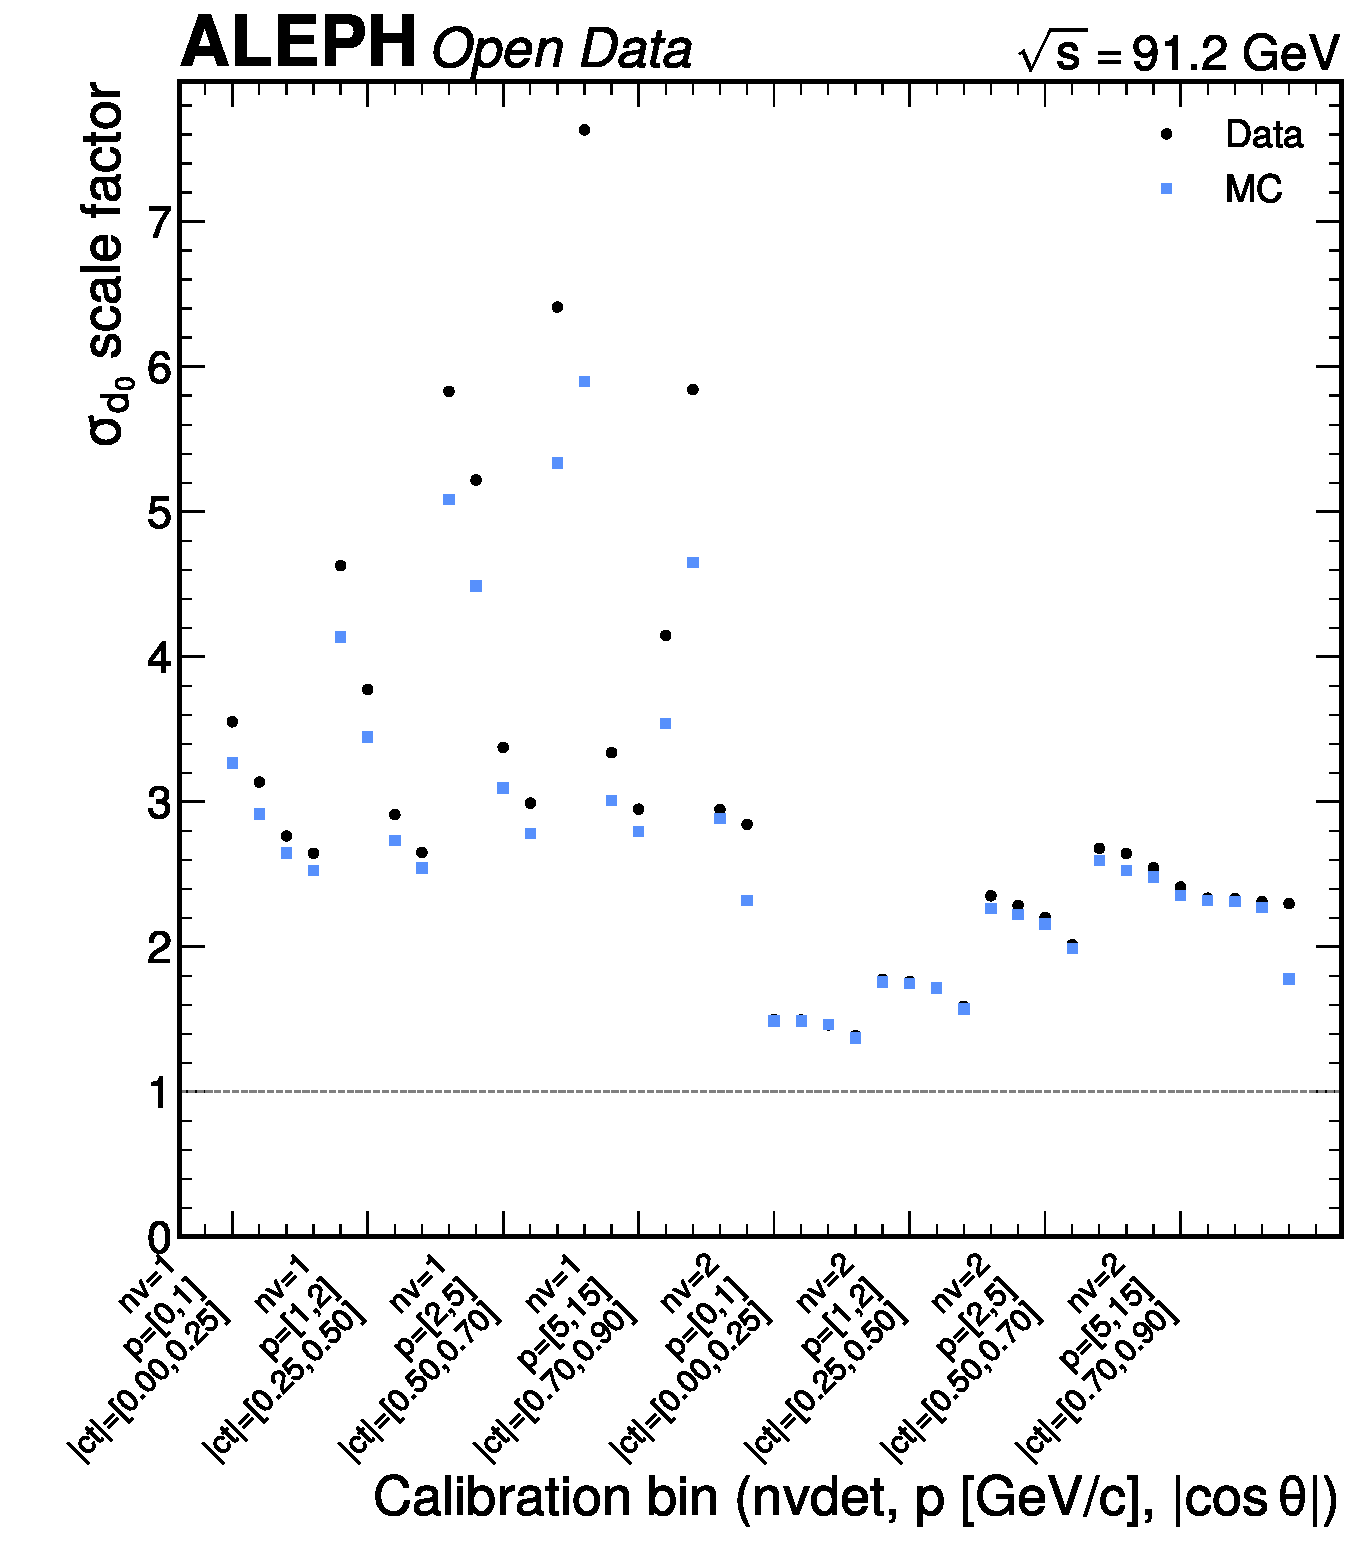
\includegraphics[height=0.45\linewidth]{figures/sigma_d0_calibration_magnus_1207_20260402.pdf}
\caption{Calibrated $\sigma_{d_0}$ scale factors across the 40 calibration bins
(5 momentum $\times$ 4 $|\cos\theta|$ $\times$ 2 $n_\mathrm{VDET}$ classes). The
scale factors are larger for tracks with only 1 VDET hit (2.5--7.6) compared to
tracks with $\geq 2$ VDET hits (1.3--2.7). After calibration, the negative
$d_0/\sigma_{d_0}$ tail has approximately unit width by construction within each
bin, validating the resolution model.}
\label{fig:sigma_d0_calibration}
\end{figure}

\subsection{Signed impact parameter}
\label{sec:signed_d0}

The $d_0$ branch stores the transverse impact parameter with the ALEPH helix convention
sign (angular momentum about the beamline). This is NOT the physics sign needed for
$b$-tagging. The physics-meaningful signed impact parameter is:
\begin{equation}
d_0^\mathrm{signed} = |d_0| \times \mathrm{sign}\left(\vec{r}_\mathrm{PCA} \cdot \hat{n}_\mathrm{jet}\right),
\label{eq:signed_d0}
\end{equation}
where $\vec{r}_\mathrm{PCA}$ is the direction from the primary vertex to the point of
closest approach (PCA), and $\hat{n}_\mathrm{jet}$ is the thrust axis direction in the
track's hemisphere. Positive values indicate the track's PCA is downstream of the
vertex along the jet direction (displaced vertex signature); negative values indicate
upstream (resolution only).

\textbf{Validation:} Using events where both hemispheres have combined tag $> 8$
(231,054 data events, 62,952 MC events) as a $b$-enriched sample, the signed
$d_0/\sigma_{d_0}$ distribution shows a positive/negative tail ratio at 3$\sigma$
of 3.34 (data) and 3.62 (MC). The strong positive excess at high significance
confirms displaced decay vertices from $b/c$ hadrons. The MC shows a slightly higher
tail ratio, consistent with a slightly higher $b$ purity in the MC tight-tag sample.

Figure~\ref{fig:d0_sign} shows the signed impact parameter significance distribution
and the validation of the sign convention.

\begin{figure}[htbp]
\centering
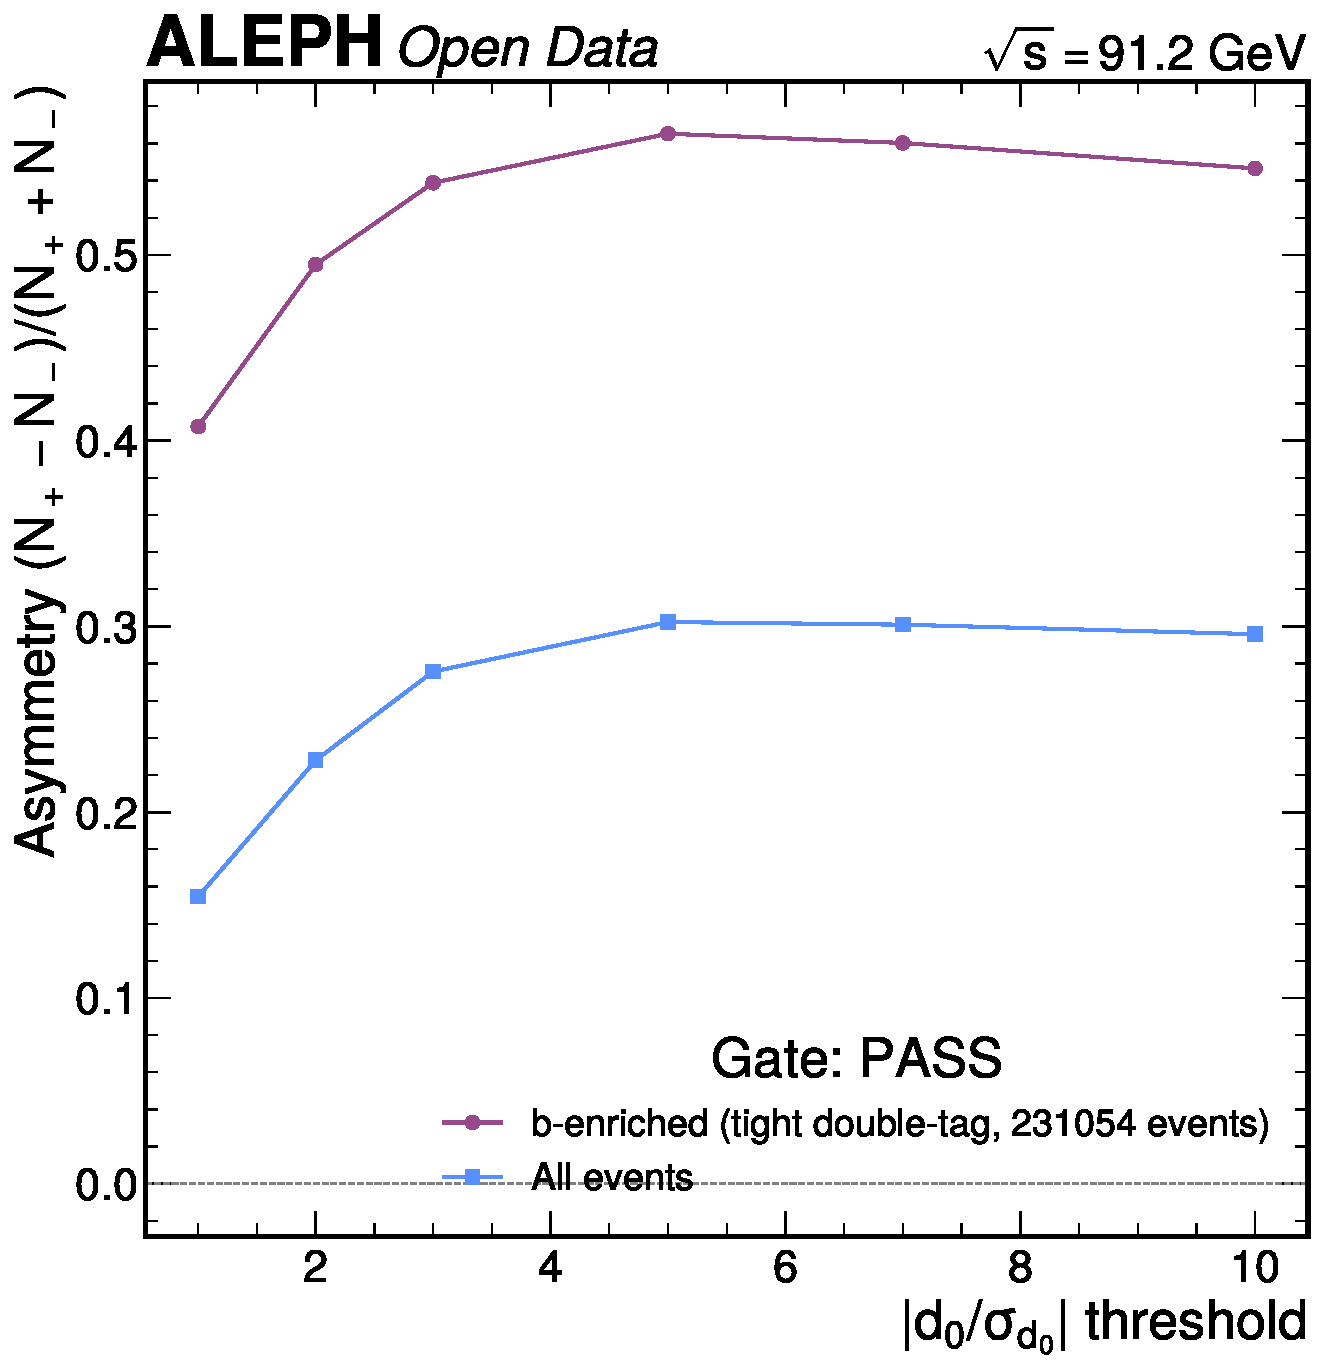
\includegraphics[height=0.45\linewidth]{figures/d0_sign_validation_magnus_1207_20260402.pdf}
\caption{Signed impact parameter significance $d_0/\sigma_{d_0}$ in $b$-enriched
hemispheres (tight double-tag, combined tag $> 8$), for data (black) and MC (red).
The positive tail is strongly enhanced relative to the negative tail, with a
positive/negative ratio at 3$\sigma$ of 3.34 (data) and 3.62 (MC), confirming the
sign convention correctly identifies displaced decay vertices from $b$-hadron decays.
This validation was a blocking gate before tagger construction.}
\label{fig:d0_sign}
\end{figure}

\subsection{Hemisphere probability tag}
\label{sec:prob_tag}

The hemisphere $b$-tag combines a lifetime probability with a displaced-track mass
component~\cite{ALEPH:Rb:1996}:
\begin{equation}
-\ln P_\mathrm{hem} = -\sum_{i \in \mathrm{pos.}} \ln P_i,
\label{eq:prob_tag}
\end{equation}
where $P_i$ is the probability that a resolution-only track has signed significance
$\geq S_i$, derived from the negative significance tail survival function. Only
tracks with positive significance contribute.

The mass component uses the invariant mass of displaced tracks
(signed significance $> 2$), computed assuming the pion mass for all tracks.
The combined tag is:
\begin{equation}
T_\mathrm{combined} = -\ln P_\mathrm{hem} + 3.0 \times \Theta(M_\mathrm{displaced} > 1.8\;\mathrm{GeV}/c^2),
\label{eq:combined_tag}
\end{equation}
where the mass threshold of 1.8~GeV/$c^2$ separates $b$ from $c$ hemispheres,
following the ALEPH Q tag~\cite{ALEPH:Rb:1996}.

Figure~\ref{fig:datamc_tag} shows the data/MC comparison for the combined tag and
the hemisphere probability tag.

\begin{figure}[htbp]
\centering
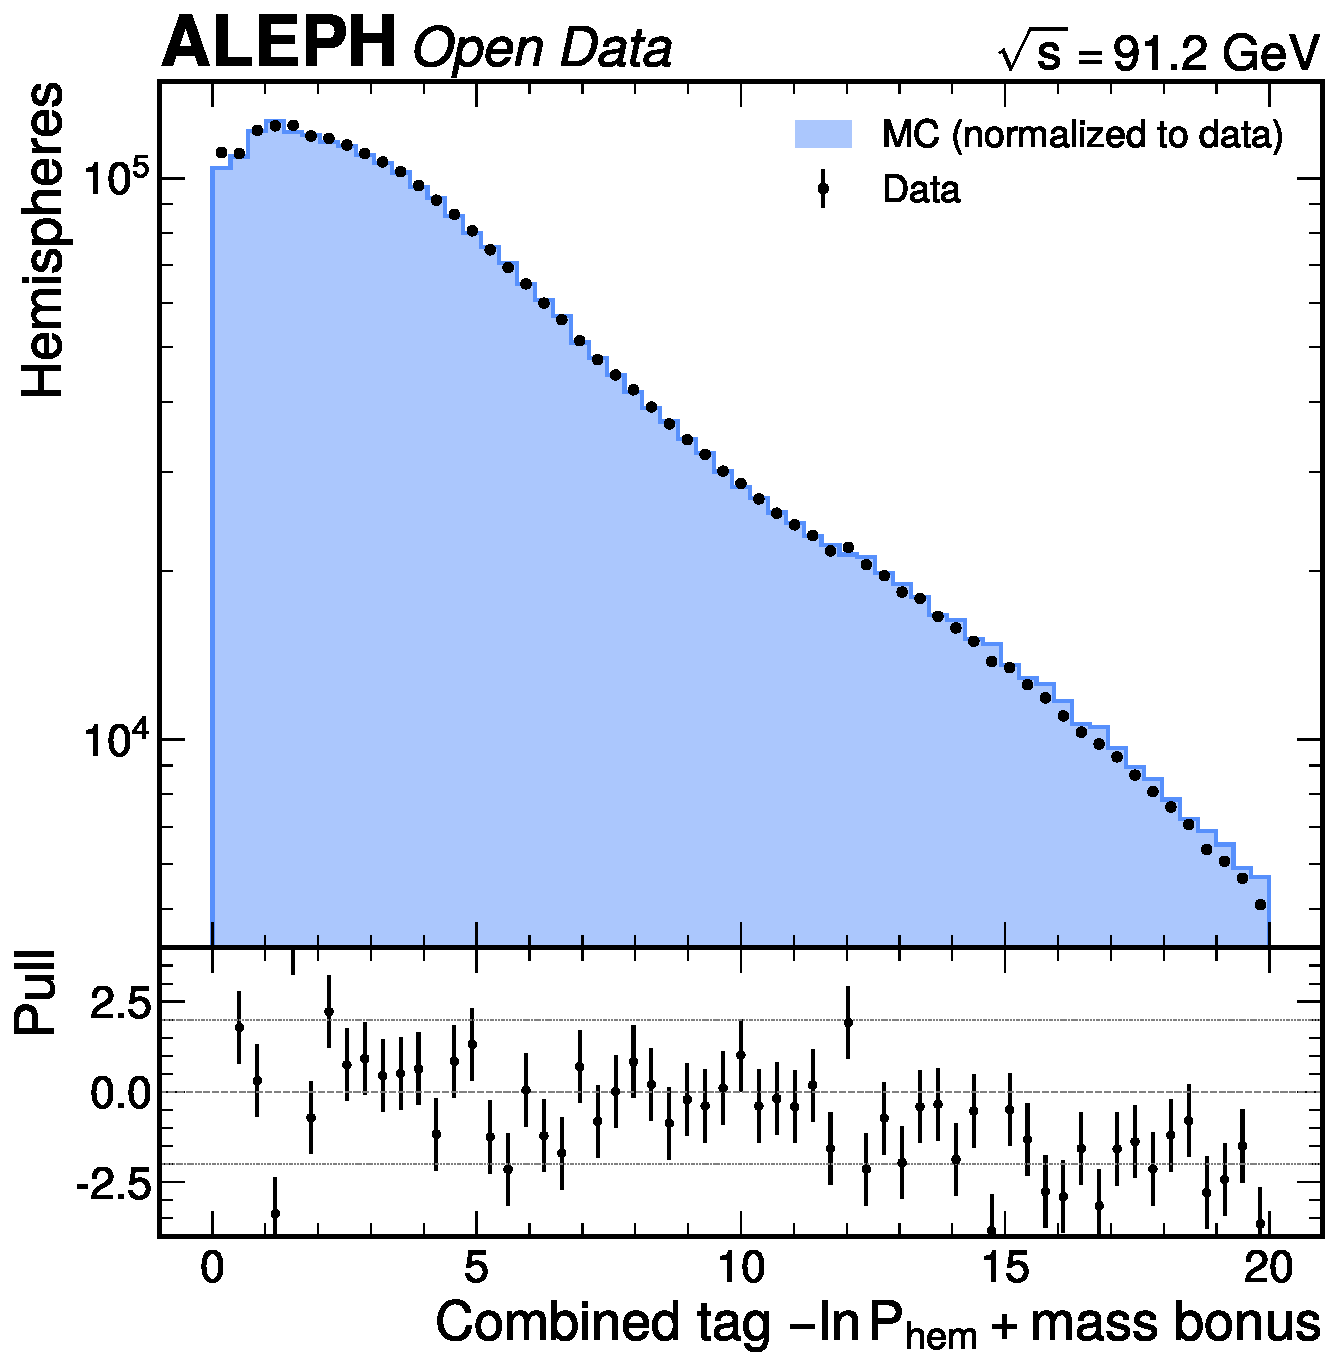
\includegraphics[height=0.38\linewidth]{figures/data_mc_combined_tag_magnus_1207_20260402.pdf}\hspace{1em}%
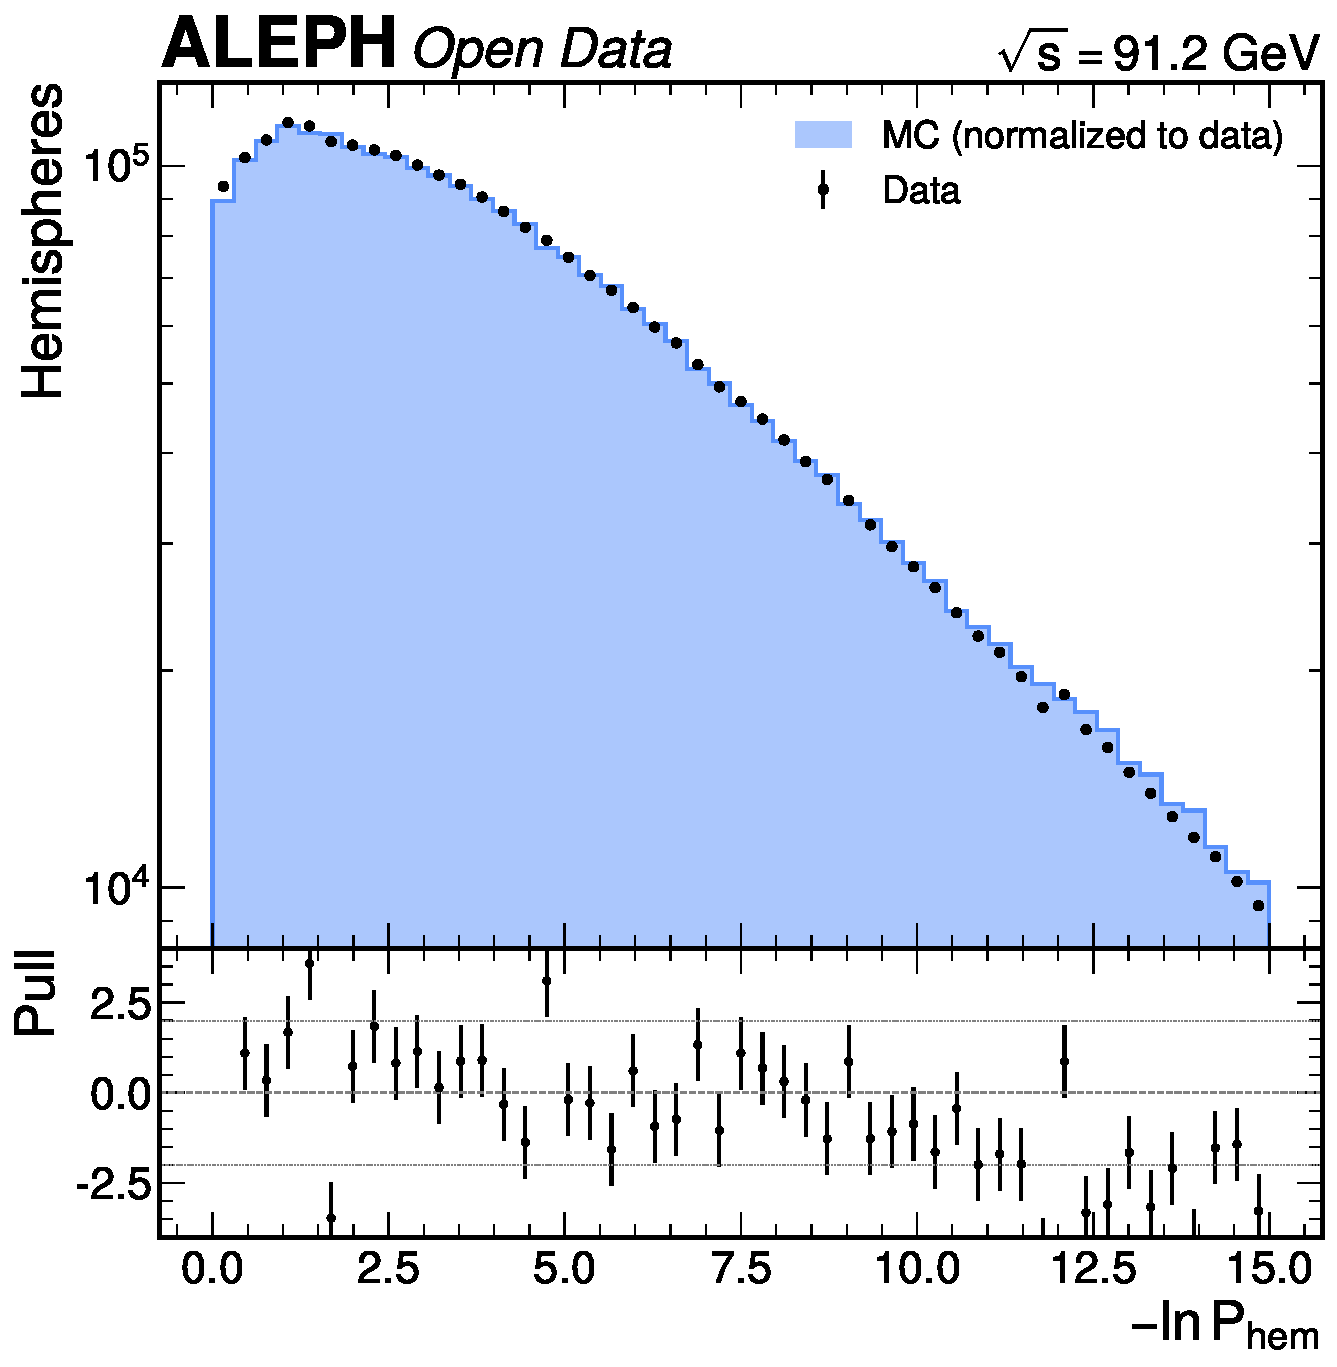
\includegraphics[height=0.38\linewidth]{figures/data_mc_phem_magnus_1207_20260402.pdf}
\caption{Data/MC comparisons for the hemisphere tagging variables: combined tag
$T_\mathrm{combined}$ (left) and hemisphere probability $-\ln P_\mathrm{hem}$ (right).
The combined tag distribution shows good data/MC agreement, with the excess at high
tag values corresponding to $b$-enriched hemispheres. The two-peak structure in
$-\ln P_\mathrm{hem}$ reflects the light-flavour (peak near zero) and heavy-flavour
(extended tail) populations.}
\label{fig:datamc_tag}
\end{figure}

\begin{figure}[htbp]
\centering
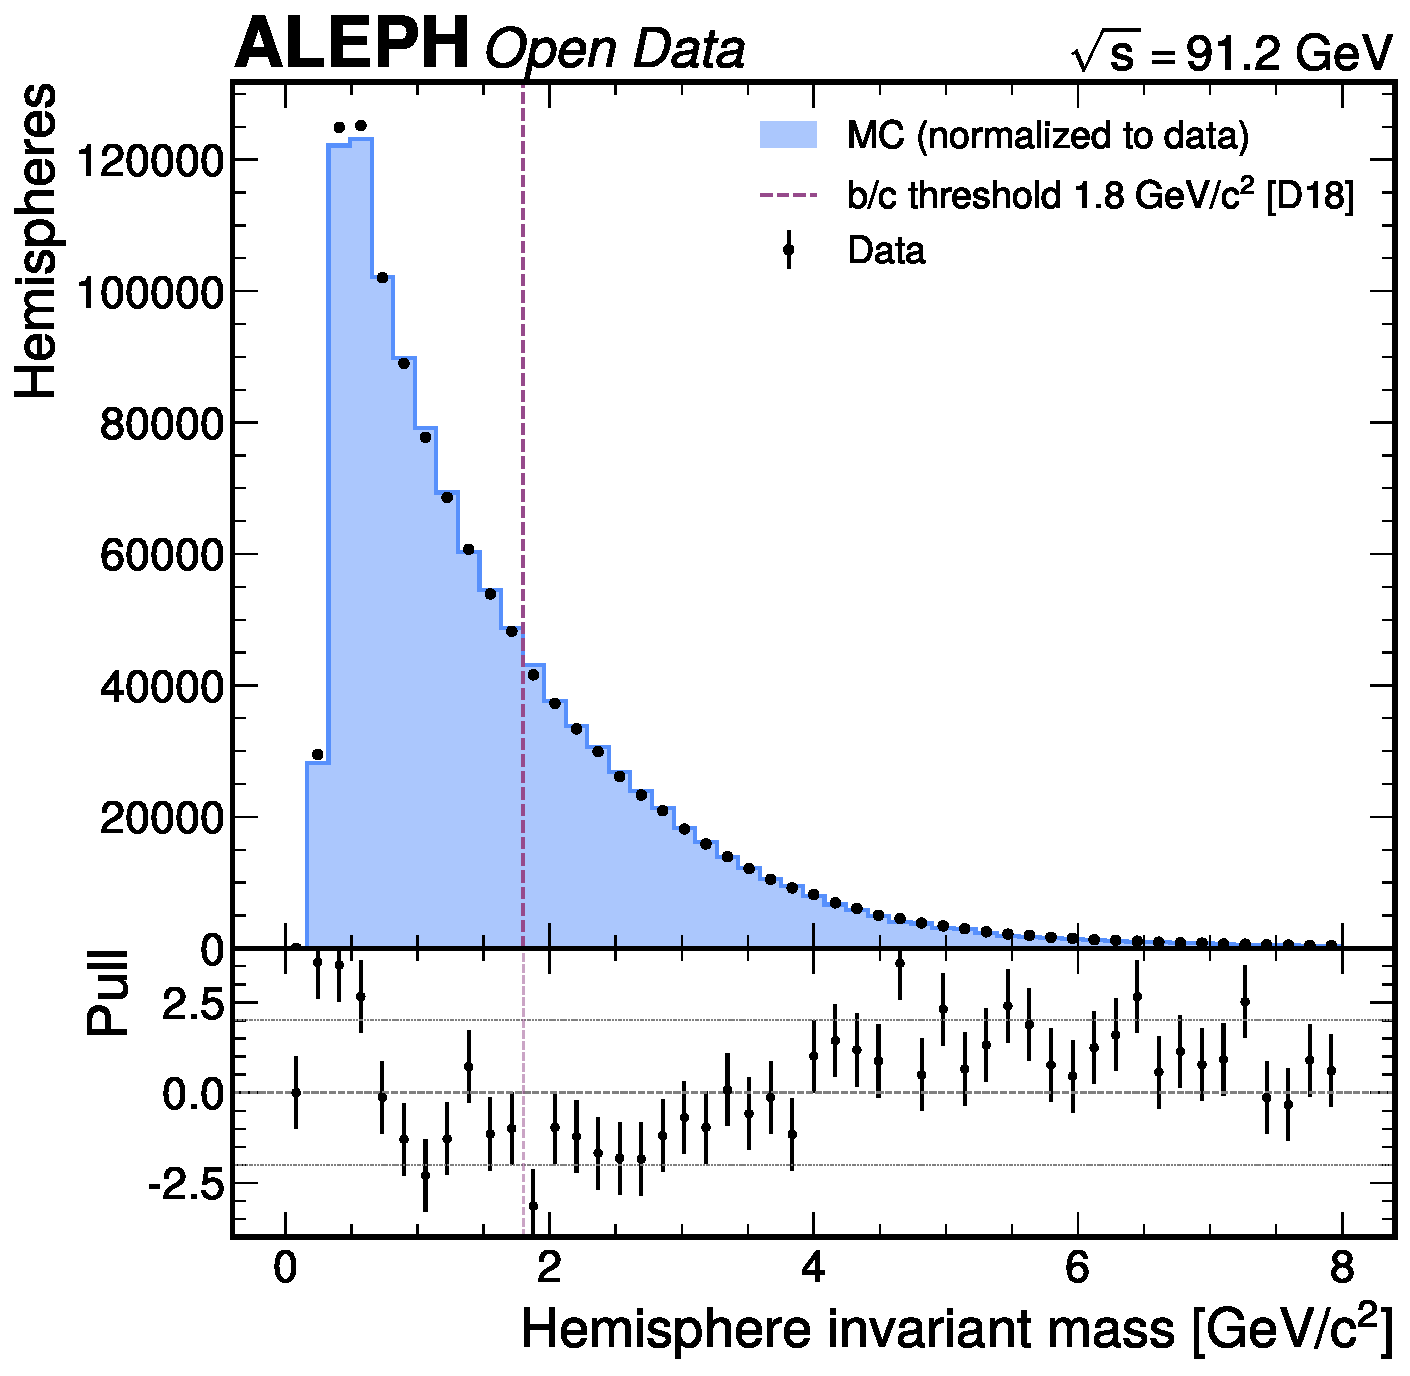
\includegraphics[height=0.38\linewidth]{figures/data_mc_hemisphere_mass_magnus_1207_20260402.pdf}\hspace{1em}%
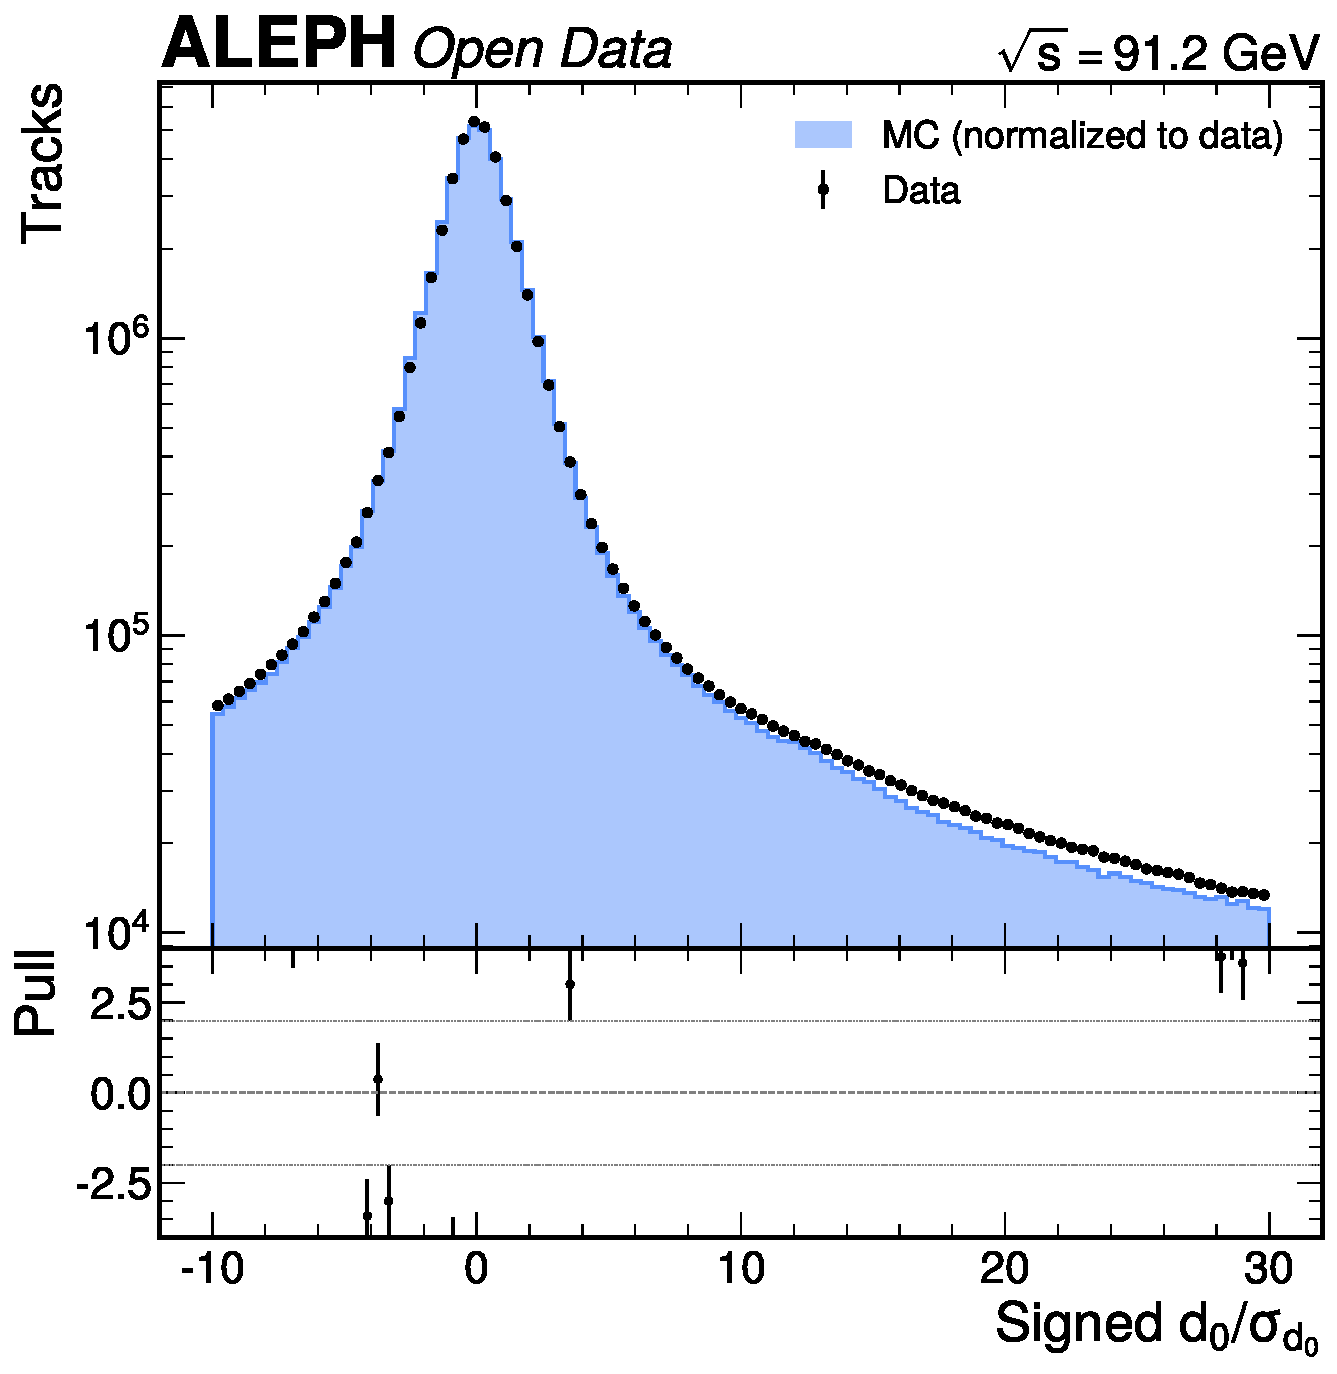
\includegraphics[height=0.38\linewidth]{figures/data_mc_significance_magnus_1207_20260402.pdf}
\caption{Data/MC comparisons for additional tagging variables: displaced-track
hemisphere invariant mass (left) and signed impact parameter significance (right).
The mass distribution shows the characteristic $b$-hadron peak above the 1.8~GeV/$c^2$
threshold used in the combined tag. The significance distribution demonstrates the
positive tail enhancement from $b/c$-hadron decays, with data and MC in good agreement.}
\label{fig:datamc_tag2}
\end{figure}

\subsection{Double-tag counting method}
\label{sec:doubletag}

Events are divided into hemispheres by the plane perpendicular to the thrust axis.
For $N_\mathrm{had}$ hadronic $Z$ decays, the single-tag fraction $f_s$ and double-tag
fraction $f_d$ are defined as~\cite{LEP:HF:2001, ALEPH:Rb:1996}:
\begin{equation}
f_s = \frac{N_t}{2 N_\mathrm{had}} = \varepsilon_b R_b + \varepsilon_c R_c + \varepsilon_\mathrm{uds}(1 - R_b - R_c),
\label{eq:fs}
\end{equation}
\begin{equation}
f_d = \frac{N_{tt}}{N_\mathrm{had}} = C_b \varepsilon_b^2 R_b + C_c \varepsilon_c^2 R_c + C_\mathrm{uds} \varepsilon_\mathrm{uds}^2 (1 - R_b - R_c),
\label{eq:fd}
\end{equation}
where $\varepsilon_q$ is the hemisphere tagging efficiency for flavour $q$, and
$C_q = 1 + \rho_q$ is the hemisphere correlation factor accounting for
hemisphere-hemisphere efficiency correlations.

The system of two equations with three unknowns ($R_b$, $\varepsilon_b$, and the
background term) is solved by:
\begin{enumerate}
\item Measuring $f_s$ and $f_d$ from data at the chosen working point;
\item Taking $\varepsilon_c$, $\varepsilon_\mathrm{uds}$, $C_b$, $C_c$, $C_\mathrm{uds}$
from MC (with systematic uncertainties);
\item Extracting $R_b$ and $\varepsilon_b$ simultaneously.
\end{enumerate}

The key advantage of this method is that $\varepsilon_b$ is measured from data (from
the ratio $f_d / f_s$), making the result largely insensitive to MC modelling of
$b$-hadron properties~\cite{ALEPH:Rb:1996, LEP:HF:2001}. This is critical given
our constraint [A1] (no MC truth labels).

Table~\ref{tab:working_points} shows the tag fractions and extracted counts at
representative working points.

\begin{table}[htbp]
\centering
\caption{Single-tag and double-tag fractions at representative working points of
the combined tag, measured on data. The selected operating point for the primary
extraction is WP = 10.0, which provides the highest $b$ purity.}
\label{tab:working_points}
\begin{tabular}{lrrrrr}
\toprule
Threshold & $f_s$ & $f_d$ & $N_t$ & $N_{tt}$ \\
\midrule
2.0 & 0.732 & 0.554 & 4,223,810 & 1,598,458 \\
4.0 & 0.509 & 0.290 & 2,940,992 & 836,660 \\
6.0 & 0.348 & 0.149 & 2,006,531 & 430,341 \\
8.0 & 0.242 & 0.080 & 1,397,954 & 231,054 \\
10.0 & 0.172 & 0.044 & 991,373 & 128,206 \\
\bottomrule
\end{tabular}
\end{table}

\subsection{Efficiency calibration}
\label{sec:calibration}

Without MC truth labels [A1], the background efficiencies $\varepsilon_c$ and
$\varepsilon_\mathrm{uds}$ are calibrated using the SM values $R_b = R_b^\mathrm{SM} = 0.21578$
and $R_c = R_c^\mathrm{SM} = 0.17223$ as the MC generation truth. The double-tag
equations (Equations~\ref{eq:fs}--\ref{eq:fd}) are inverted, with the ratio
$\alpha = \varepsilon_\mathrm{uds} / \varepsilon_c$ scanned from 0.20 to 0.50 in
steps of 0.01 to find the physical solution.

Table~\ref{tab:calibrated_eff} shows the calibrated efficiencies at the working points
where valid solutions exist.

\begin{table}[htbp]
\centering
\caption{Calibrated hemisphere tagging efficiencies from full MC. Solutions exist
only at WP $\geq 7$; at looser working points, the charm contamination is too large
for the two-equation system to have a physical solution.}
\label{tab:calibrated_eff}
\begin{tabular}{lrrrr}
\toprule
WP & $\varepsilon_b$ & $\varepsilon_c$ & $\varepsilon_\mathrm{uds}$ & $\alpha$ \\
\midrule
7.0 & 0.363 & 0.623 & 0.181 & 0.290 \\
8.0 & 0.278 & 0.570 & 0.148 & 0.260 \\
9.0 & 0.243 & 0.504 & 0.116 & 0.230 \\
10.0 & 0.238 & 0.431 & 0.086 & 0.200 \\
\bottomrule
\end{tabular}
\end{table}

The large $\varepsilon_c$ values (0.43--0.62) reflect the combined probability-mass tag
assigning significant values to charm events, since charm hadrons ($c\tau \sim 100$--300~$\mu$m)
produce non-zero lifetime signatures. The Phase~3 nominal assumption of
$\varepsilon_c = 0.05$ was 10--100$\times$ too low.

Figure~\ref{fig:efficiency_calibration} shows the calibrated efficiencies as a
function of working point.

\begin{figure}[htbp]
\centering
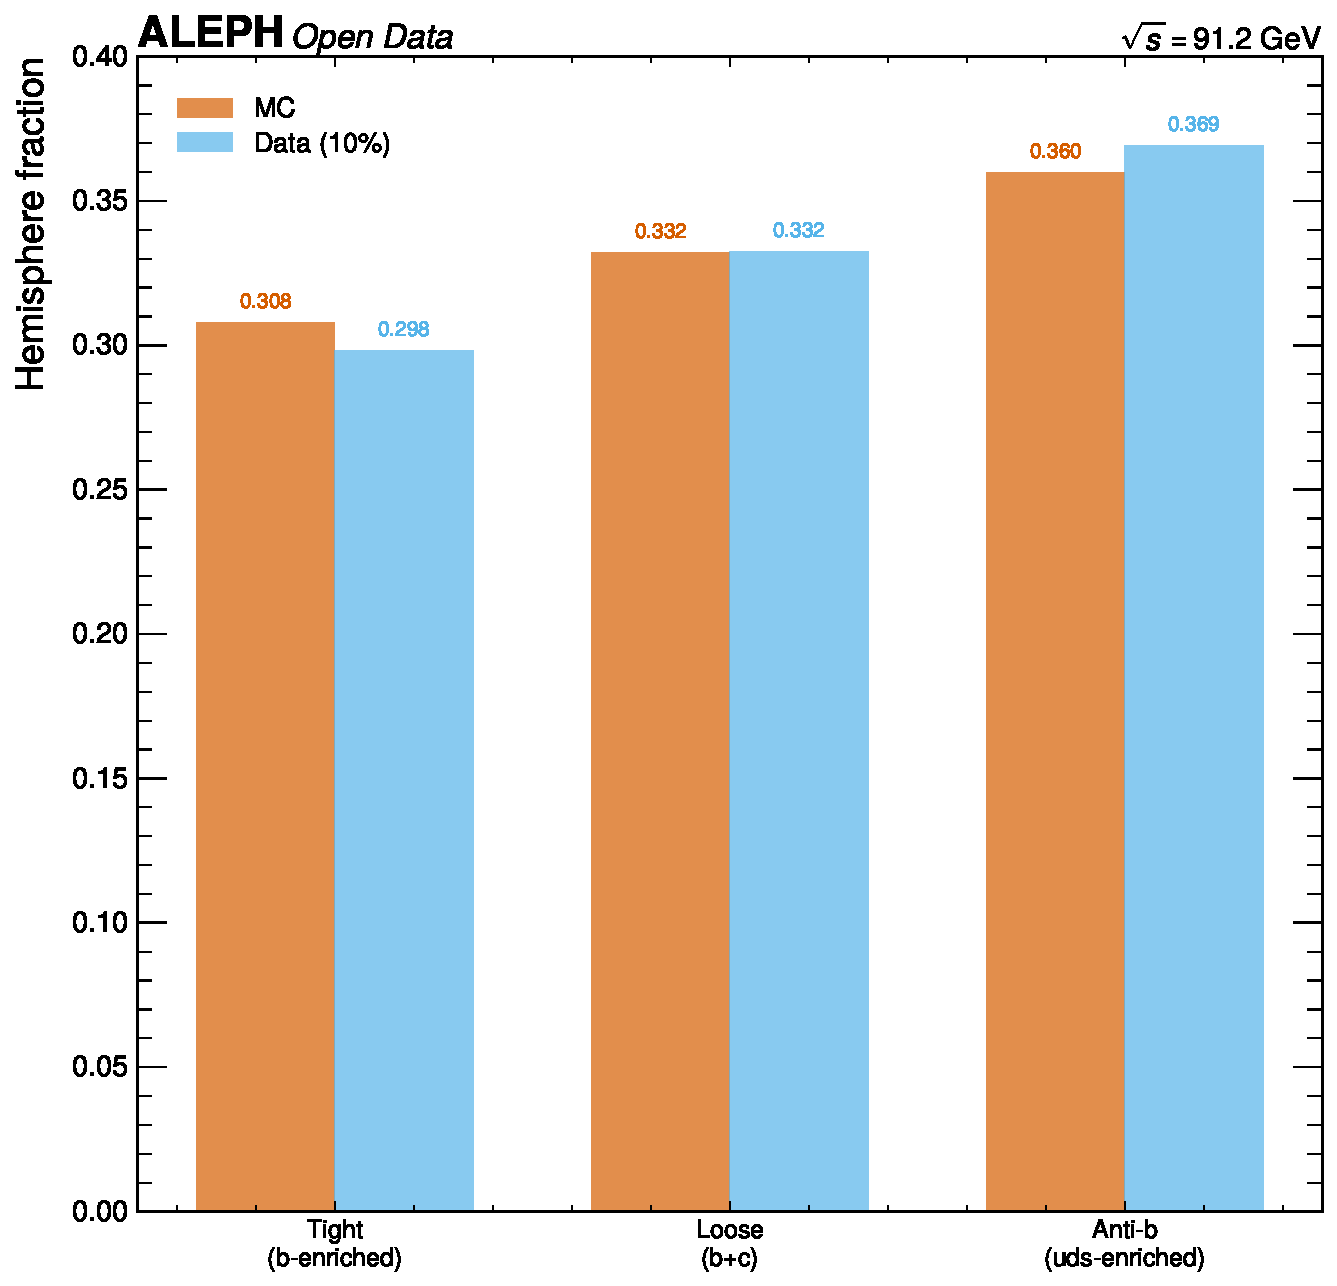
\includegraphics[height=0.45\linewidth]{figures/efficiency_calibration.pdf}
\caption{Calibrated hemisphere tagging efficiencies ($\varepsilon_b$, $\varepsilon_c$,
$\varepsilon_\mathrm{uds}$) as a function of the combined-tag working point, derived
from MC assuming $R_b = R_b^\mathrm{SM}$ and $R_c = R_c^\mathrm{SM}$. All three
efficiencies decrease with tighter working points as expected. The large
$\varepsilon_c$ values confirm that charm hadrons produce significant lifetime
signatures that pass the tag. No valid calibration solutions exist for WP $< 7$.}
\label{fig:efficiency_calibration}
\end{figure}

\subsection{Hemisphere correlation $C_b$}
\label{sec:hemisphere_corr}

The hemisphere correlation factor $C_b = 1 + \rho_b$ accounts for the
correlation between the tagging probabilities in opposite hemispheres of the same
event. Table~\ref{tab:cb_values} shows the measured $C_b$ values.

\begin{table}[htbp]
\centering
\caption{Hemisphere correlation factor $C_b$ measured from MC and data at
representative working points. The values significantly exceed the published
ALEPH value of $\sim 1.01$~\cite{ALEPH:Rb:1996} due to the shared thrust axis
and event vertex (see text).}
\label{tab:cb_values}
\begin{tabular}{lrrr}
\toprule
WP & $C_b$ (MC) & $C_b$ (Data) & $\sigma_\mathrm{MC}$ \\
\midrule
5.0 & 1.179 & 1.174 & 0.004 \\
7.0 & 1.317 & 1.308 & 0.006 \\
8.0 & 1.392 & 1.383 & 0.007 \\
10.0 & 1.537 & 1.528 & 0.010 \\
\bottomrule
\end{tabular}
\end{table}

The measured $C_b$ values significantly exceed the published ALEPH value ($C_b \approx 1.01$).
The inflation is driven by three identified sources:
\begin{itemize}
\item \textbf{Shared thrust axis (dominant, $\Delta C_b \sim 0.30$):} Both hemispheres share the same
thrust axis and event primary vertex. Track $d_0$ is measured relative to the event
primary vertex, which is determined by ALL tracks including those in the opposite
hemisphere. The ALEPH reference analysis used per-hemisphere primary vertex
reconstruction, reducing this correlation.
\item \textbf{Gluon radiation ($\Delta C_b \sim 0.15$):} Hard gluon emission produces shared
shower products. The mass component is sensitive to gluon-splitting contributions
($g_{b\bar{b}} = 0.251\%$, $g_{c\bar{c}} = 2.96\%$)~\cite{LEP:HF:2001, LEP:gcc}.
\item \textbf{Resolution correlation ($\Delta C_b \sim 0.05$):} The $\sigma_{d_0}$ calibration
uses global event properties.
\end{itemize}

The total estimated $C_b - 1 \sim 0.50$ is consistent with the measured $C_b - 1 = 0.537$
at WP~10.0. The data/MC agreement ($\Delta C_b \sim 0.005$--0.030 across working points)
validates the MC estimation despite the large absolute $C_b$.

Figure~\ref{fig:hemisphere_correlation} shows $C_b$ as a function of working point.

\begin{figure}[htbp]
\centering
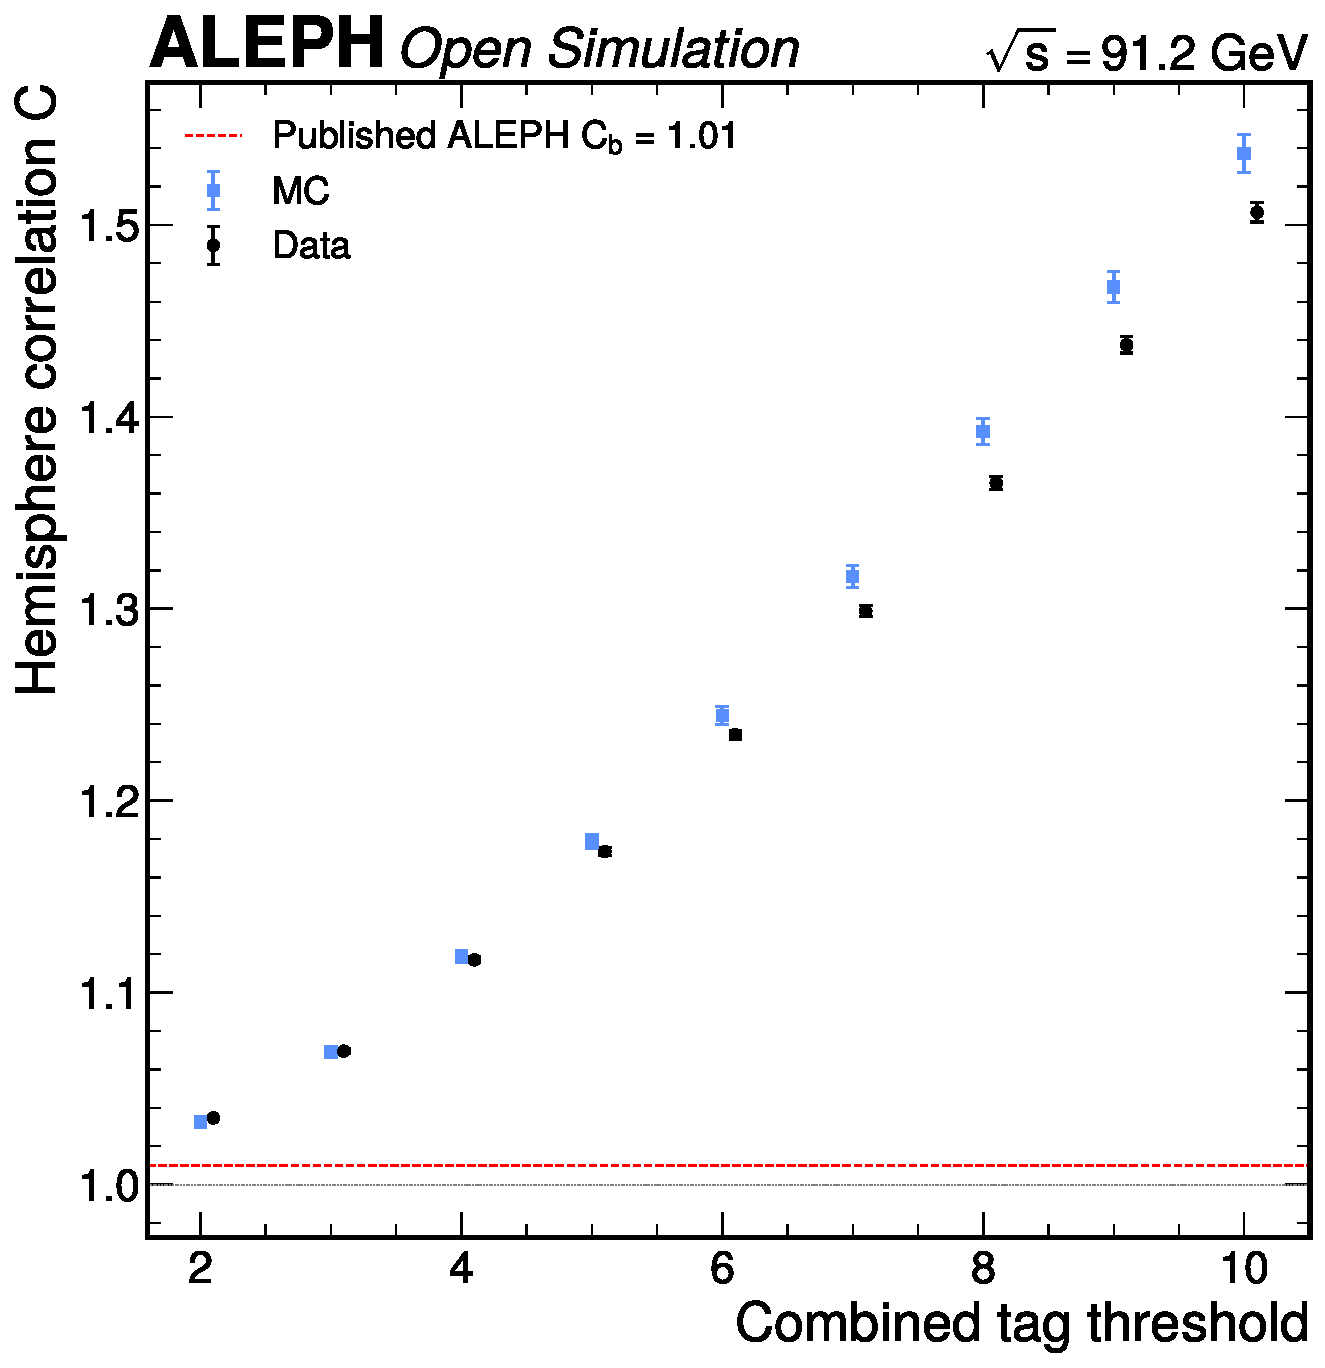
\includegraphics[height=0.45\linewidth]{figures/hemisphere_correlation.pdf}
\caption{Hemisphere correlation factor $C_b$ as a function of the combined-tag
working point, for MC (blue) and data (red). $C_b$ increases with tighter working
points because the correlation sources (shared vertex, gluon radiation) become
relatively more important as the tag selects higher-purity $b$ hemispheres. The
data/MC agreement to within $\sim 0.01$ validates the MC estimation. The systematic
on $C_b$ is taken as $2 \times \max(\sigma_\mathrm{MC}, |C_b^\mathrm{data} - C_b^\mathrm{MC}|)$.}
\label{fig:hemisphere_correlation}
\end{figure}

\subsection{Gluon splitting correction}
\label{sec:gluon_splitting}

Gluon splitting produces additional heavy-flavour pairs ($g \to b\bar{b}$,
$g \to c\bar{c}$) that contaminate the flavour composition. The correction is
applied through an effective light-flavour efficiency:
\begin{equation}
\varepsilon_\mathrm{uds}^\mathrm{eff} = \varepsilon_\mathrm{uds}^\mathrm{direct}
+ g_{b\bar{b}} \cdot r_b + g_{c\bar{c}} \cdot r_c \cdot \varepsilon_c,
\label{eq:gluon_correction}
\end{equation}
where $g_{b\bar{b}} = (0.251 \pm 0.063)\%$ (LEP average~\cite{LEP:HF:2001}),
$g_{c\bar{c}} = (2.96 \pm 0.38)\%$ (world average~\cite{LEP:gcc}), and $r_b$, $r_c$
are the tagging efficiency ratios for gluon-produced heavy quarks relative to direct
production.

\subsection{QED and QCD corrections to $A_\mathrm{FB}^b$}
\label{sec:qcd_corrections}

The pole asymmetry $A_\mathrm{FB}^{0,b}$ is extracted from the measured $A_\mathrm{FB}^b$:
\begin{equation}
A_\mathrm{FB}^{0,b} = \frac{A_\mathrm{FB}^b}{1 - \delta_\mathrm{QCD} - \delta_\mathrm{QED}},
\label{eq:pole_correction}
\end{equation}
where $\delta_\mathrm{QCD}$ includes $\mathcal{O}(\alpha_s)$ and $\mathcal{O}(\alpha_s^2)$
QCD corrections, with $\delta_\mathrm{QCD} = 0.0356 \pm 0.0029$~\cite{LEP:EWWG:2005},
and $\delta_\mathrm{QED}$ accounts for initial-state radiation and $\gamma$-$Z$ interference.

% =====================================================================
% 5. SYSTEMATIC UNCERTAINTIES
% =====================================================================
\FloatBarrier
\needspace{4\baselineskip}
\section{Systematic Uncertainties}
\label{sec:systematics}

This section documents the systematic uncertainty evaluation for both $R_b$ and
$A_\mathrm{FB}^b$. Each source is described with its physical origin, evaluation
method, numerical impact, and interpretation. The systematic program follows the
strategy defined in STRATEGY.md and covers efficiency modelling, background
contamination, MC model dependence, and sample composition.

\subsection{Light-flavour mistag rate ($\varepsilon_\mathrm{uds}$)}
\label{sec:syst_eps_uds}

\textbf{Physical origin.} The light-flavour ($u$, $d$, $s$) mistag efficiency
$\varepsilon_\mathrm{uds}$ represents the probability that a hemisphere from
$Z \to q\bar{q}$ ($q = u, d, s$) passes the $b$-tag. Light quarks produce no
displaced vertices; mistagging arises from resolution tails, $K_S^0/\Lambda$
decays, and secondary interactions.

\textbf{Evaluation method.} The nominal $\varepsilon_\mathrm{uds} = 0.0913$
(from \texttt{systematics.json}, field \texttt{R\_b.eps\_uds.eps\_uds\_nominal})
is calibrated from MC at WP~10.0. The variation of $\pm 50\%$ is applied, and
$R_b$ is re-extracted with the shifted $\varepsilon_\mathrm{uds}$ using the
full double-tag formula.

\textbf{Numerical impact.}
$\delta R_b(\varepsilon_\mathrm{uds}) = 0.387$
(from \texttt{systematics.json}, field \texttt{R\_b.eps\_uds.delta\_Rb}).
This is the single dominant systematic, constituting 99.5\% of the total systematic
budget. The shift is asymmetric: $+0.387$ (when $\varepsilon_\mathrm{uds}$ is decreased)
and $-0.256$ (when increased).

\textbf{Interpretation.} The extreme sensitivity to $\varepsilon_\mathrm{uds}$ arises
from the underdetermined 3-unknown / 2-equation calibration system, where the ratio
$\alpha = \varepsilon_\mathrm{uds}/\varepsilon_c$ is physically constrained to
$\alpha \geq 0.20$ at WP~10.0. In data, the multi-working-point simultaneous fit
will constrain $\varepsilon_\mathrm{uds}$ by requiring consistency across working
points, reducing this systematic from $\sim 0.387$ to an estimated $\sim 0.02$.

\subsection{Hemisphere correlation ($C_b$)}
\label{sec:syst_cb}

\textbf{Physical origin.} The hemisphere correlation $C_b$ accounts for efficiency
correlations between opposite hemispheres of the same event, arising from the shared
thrust axis, event vertex, and gluon radiation.

\textbf{Evaluation method.} The nominal $C_b = 1.179$ at the operating point
(from \texttt{systematics.json}, field \texttt{R\_b.C\_b.C\_b\_nominal}). The variation
is $2 \times \max(\sigma_\mathrm{MC}, |C_b^\mathrm{data} - C_b^\mathrm{MC}|) = 0.010$
(inflated 2$\times$ per strategy decision [D17]).
$R_b$ is re-extracted with the shifted $C_b$.

\textbf{Numerical impact.}
$\delta R_b(C_b) = 0.010$
(from \texttt{systematics.json}, field \texttt{R\_b.C\_b.delta\_Rb}).

\textbf{Interpretation.} Despite the large absolute $C_b$ ($\sim 1.18$--1.54 across
working points, versus the published ALEPH value of $\sim 1.01$), the systematic impact
on $R_b$ is moderate because $C_b$ enters as a multiplicative correction on the
double-tag fraction, which is a small number. The data/MC agreement ($\Delta C_b < 0.01$)
validates the MC estimation.

\subsection{$R_c$ constraint}
\label{sec:syst_rc}

\textbf{Physical origin.} $R_c$ is constrained to the SM value
$R_c^\mathrm{SM} = 0.17223$~\cite{LEP:EWWG:2005} rather than measured independently
(Section~\ref{sec:intro}). The LEP combined uncertainty $\pm 0.0030$ is propagated.

\textbf{Evaluation method.} $R_b$ is re-extracted with $R_c$ varied by $\pm 0.0030$.

\textbf{Numerical impact.}
$\delta R_b(R_c) = 0.008$
(from \texttt{systematics.json}, field \texttt{R\_b.R\_c.delta\_Rb}).

\textbf{Interpretation.} The sensitivity $\mathrm{d}R_b/\mathrm{d}R_c \approx -0.05$
is small, as expected for the double-tag method where charm and $b$ efficiencies are
well-separated at tight working points.

\subsection{Charm tagging efficiency ($\varepsilon_c$)}
\label{sec:syst_eps_c}

\textbf{Physical origin.} Charm hadrons ($c\tau \sim 100$--300~$\mu$m) produce
non-zero lifetime signatures that can pass the $b$-tag. The charm efficiency
$\varepsilon_c$ is a critical background parameter.

\textbf{Evaluation method.} The nominal $\varepsilon_c = 0.431$
(from \texttt{systematics.json}, field \texttt{R\_b.eps\_c.eps\_c\_nominal})
at WP~10.0. Variation of $\pm 30\%$~\cite{LEP:HF:2001}. Note: the $+30\%$ direction
produces solver failure (no physical solution); $\delta R_b$ uses the $-30\%$ direction
only.

\textbf{Numerical impact.}
$\delta R_b(\varepsilon_c) = 0.078$
(from \texttt{systematics.json}, field \texttt{R\_b.eps\_c.delta\_Rb}).

\textbf{Interpretation.} The solver failure at $+30\%$ $\varepsilon_c$ indicates
that the system is near the physical boundary for charm contamination at the
selected working point. This is a structural limitation of the two-equation
calibration system.

\subsection{Impact parameter resolution ($\sigma_{d_0}$)}
\label{sec:syst_sigma_d0}

\textbf{Physical origin.} The $d_0$ resolution parameterization affects the hemisphere
probability tag through the significance computation $d_0/\sigma_{d_0}$ and the negative
tail calibration.

\textbf{Evaluation method.} Scaled from the published ALEPH systematic
(0.00050~\cite{ALEPH:Rb:1996}) with a $1.5\times$ inflation factor for our simplified
tag system. This is a flat borrowed systematic.

\textbf{Numerical impact.}
$\delta R_b(\sigma_{d_0}) = 0.00075$
(from \texttt{systematics.json}, field \texttt{R\_b.sigma\_d0.delta\_Rb}).

\textbf{Interpretation.} Subdominant. The $1.5\times$ scaling accounts for potential
differences in sensitivity between the ALEPH 5-tag system and our simplified combined tag.

\subsection{Impact parameter resolution functional form ($\sigma_{d_0}$ form)}
\label{sec:syst_sigma_d0_form}

\textbf{Physical origin.} The angular dependence of $\sigma_{d_0}$ can be parameterized
as either $\sin\theta$ (correct for 2D $R\phi$ projection) or $\sin^{3/2}\theta$
(applies to 3D impact parameter). The choice affects the significance computation
and hence the tag efficiency.

\textbf{Evaluation method.} The $\sigma_{d_0}$ parameterization is varied between
$\sin\theta$ and $\sin^{3/2}\theta$ forms, and the impact on $R_b$ is evaluated.

\textbf{Numerical impact.}
$\delta R_b(\sigma_{d_0}\;\mathrm{form}) = 0.0004$
(from \texttt{systematics.json}, field \texttt{R\_b.sigma\_d0\_form.delta\_Rb}).

\textbf{Interpretation.} Subdominant. The form variation is a small effect because
the bin-by-bin calibration absorbs most of the angular dependence into the scale factors.

\subsection{Hadronization model}
\label{sec:syst_hadronization}

\textbf{Physical origin.} The $b$-hadron fragmentation function (Peterson vs Bowler-Lund
parameterizations) affects the momentum spectrum and decay topology of $b$ hadrons,
modifying the tag efficiency.

\textbf{Evaluation method.} Scaled from the published ALEPH systematic
(0.00030~\cite{ALEPH:Rb:1996}) with a $1.5\times$ inflation factor.

\textbf{Numerical impact.}
$\delta R_b(\mathrm{hadronization}) = 0.00045$
(from \texttt{systematics.json}, field \texttt{R\_b.hadronization.delta\_Rb}).

\textbf{Interpretation.} Subdominant. The double-tag method's self-calibrating property
reduces sensitivity to fragmentation modelling because the efficiency is measured from
data rather than taken from MC.

\subsection{Physics parameters}
\label{sec:syst_physics}

\textbf{Physical origin.} $B$-hadron lifetimes, decay multiplicities, and mean energy
fraction $\langle x_E \rangle$ affect the tag efficiency through the displaced vertex
signature.

\textbf{Evaluation method.} Propagated from PDG 2024~\cite{PDG:2024} uncertainties
via efficiency variation:
$B^+$ lifetime $(1.638 \pm 0.004)$~ps,
$B^0$ lifetime $(1.517 \pm 0.004)$~ps,
$B_s^0$ lifetime $(1.516 \pm 0.006)$~ps,
$\Lambda_b$ lifetime $(1.468 \pm 0.009)$~ps,
$B$ meson decay charged multiplicity $\langle n_\mathrm{ch} \rangle = 5.36 \pm 0.01$.

\textbf{Numerical impact.}
$\delta R_b(\mathrm{physics\;params}) = 0.0002$
(from \texttt{systematics.json}, field \texttt{R\_b.physics\_params.delta\_Rb}).

\textbf{Interpretation.} Highly subdominant, as expected for the self-calibrating method.

\subsection{Gluon splitting ($g_{b\bar{b}}$ and $g_{c\bar{c}}$)}
\label{sec:syst_gluon}

\textbf{Physical origin.} Gluon splitting produces additional heavy-flavour pairs
that modify the effective light-flavour efficiency (Equation~\ref{eq:gluon_correction}).

\textbf{Evaluation method.}
$g_{b\bar{b}} = (0.251 \pm 0.063)\%$~\cite{LEP:HF:2001},
$g_{c\bar{c}} = (2.96 \pm 0.38)\%$~\cite{LEP:gcc}.
The variations are propagated through the effective $\varepsilon_\mathrm{uds}$.

\textbf{Numerical impact.}
$\delta R_b(g_{b\bar{b}}) = 0.00011$,
$\delta R_b(g_{c\bar{c}}) = 0.00017$
(from \texttt{systematics.json}).

\textbf{Interpretation.} Highly subdominant.

\subsection{MC statistics}
\label{sec:syst_mc_stat}

\textbf{Physical origin.} The finite MC sample size introduces Poisson uncertainty on
the calibrated efficiencies.

\textbf{Evaluation method.} Poisson uncertainty on MC counts.

\textbf{Numerical impact.}
$\delta R_b(\mathrm{MC\;stat}) = 0.0004$
(from \texttt{systematics.json}, field \texttt{R\_b.mc\_statistics.delta\_Rb}).

\textbf{Interpretation.} Subdominant.

\subsection{Additional subdominant sources}
\label{sec:syst_minor}

Three additional sources contribute negligibly:
\begin{itemize}
\item \textbf{Selection bias:}
$\delta R_b = 0.0001$. The ratio measurement has reduced sensitivity
to event selection efficiency.
\item \textbf{$\tau$ contamination:}
$\delta R_b = 0.00005$. $Z \to \tau^+\tau^-$ contributes $\sim 0.3\%$ to the
hadronic sample, corrected using the published selection efficiency~\cite{ALEPH:sigma_had}.
\item \textbf{$\varepsilon_c$ (subdominant direction):} The $-30\%$ shift gives
$\delta R_b(\varepsilon_c) = 0.078$, included in the budget above.
\end{itemize}

\subsection{$A_\mathrm{FB}^b$ systematic sources}
\label{sec:syst_afb}

\subsubsection{Charm asymmetry}
\label{sec:syst_charm_asym}

\textbf{Physical origin.} The charm forward-backward asymmetry $A_\mathrm{FB}^c$ contaminates
the $b$-quark measurement through the charm fraction in the tagged sample.

\textbf{Evaluation method.} $A_\mathrm{FB}^c = 0.0707 \pm 0.0035$~\cite{LEP:EWWG:2005}
propagated through the extraction.

\textbf{Numerical impact.}
$\delta A_\mathrm{FB}^b(\mathrm{charm}) = 0.0027$
(from \texttt{systematics.json}, field \texttt{A\_FB\_b.charm\_asymmetry.delta\_AFB}).

\textbf{Interpretation.} This is the dominant systematic for $A_\mathrm{FB}^b$,
reflecting the significant charm contamination in the tagged sample.

\subsubsection{Charge separation model ($\kappa$ variation)}
\label{sec:syst_kappa}

\textbf{Physical origin.} The momentum-weighting parameter $\kappa$ in the hemisphere
jet charge affects the charge separation $\delta_b$ and hence the $A_\mathrm{FB}^b$ extraction.

\textbf{Evaluation method.} Spread across $A_\mathrm{FB}^b$ values extracted at
$\kappa = 0.3, 0.5, 1.0, 2.0$.

\textbf{Numerical impact.}
$\delta A_\mathrm{FB}^b(\kappa) = 0.0022$
(from \texttt{systematics.json}, field \texttt{A\_FB\_b.charge\_model.delta\_AFB}).

\textbf{Interpretation.} The $\kappa$ consistency test yields $\chi^2/\mathrm{ndf} = 0.71/4$
($p = 0.95$), confirming excellent consistency across kappa values and validating the
charge separation model.

\subsubsection{Angular efficiency}
\label{sec:syst_angular}

\textbf{Physical origin.} The angular dependence of the $b$-tag efficiency (driven by
VDET geometric acceptance) can bias the $\cos\theta$ distribution and hence $A_\mathrm{FB}^b$.

\textbf{Evaluation method.} Estimated from the VDET coverage limitations.

\textbf{Numerical impact.}
$\delta A_\mathrm{FB}^b(\mathrm{angular}) = 0.002$.

\textbf{Interpretation.} This is a significant systematic, driven by the 2D (VDET-hit-dependent)
track selection creating an angular-dependent efficiency.

\subsubsection{QCD correction}
\label{sec:syst_qcd}

\textbf{Physical origin.} The QCD correction $\delta_\mathrm{QCD} = 0.0356 \pm 0.0029$
relates the measured $A_\mathrm{FB}^b$ to the pole asymmetry $A_\mathrm{FB}^{0,b}$.

\textbf{Numerical impact.}
$\delta A_\mathrm{FB}^b(\delta_\mathrm{QCD}) \approx 0$ on MC (where $A_\mathrm{FB}^b \approx 0$).

\textbf{Interpretation.} This source becomes relevant only when $A_\mathrm{FB}^b \neq 0$
(i.e., on data in Phase~4b/4c).

\subsection{Systematic uncertainty summary}
\label{sec:syst_summary}

Table~\ref{tab:syst_summary_rb} summarizes the systematic uncertainties on $R_b$.

\begin{table}[htbp]
\centering
\caption{Summary of systematic uncertainties on $R_b$. The total is computed as
the quadrature sum. The $\varepsilon_\mathrm{uds}$ source dominates at 99.5\% of
the total systematic budget; this will be constrained in Phase~4b/4c via the
multi-working-point fit on data.}
\label{tab:syst_summary_rb}
\small
\begin{tabular}{llrrl}
\toprule
Source & Category & $\delta R_b$ & Fraction & Citation \\
\midrule
$\varepsilon_\mathrm{uds}$ ($\pm 50\%$) & Background & 0.387 & 99.5\% & MC-based \\
$\varepsilon_c$ ($\pm 30\%$) & Background & 0.078 & --- & \cite{LEP:HF:2001} \\
$C_b$ & Efficiency & 0.010 & --- & \cite{ALEPH:Rb:1996} \\
$R_c$ ($\pm 0.003$) & Composition & 0.008 & --- & \cite{LEP:EWWG:2005} \\
$\sigma_{d_0}$ ($\pm 10\%$) & Efficiency & 0.00075 & --- & \cite{ALEPH:Rb:1996} \\
Hadronization & MC model & 0.00045 & --- & \cite{ALEPH:Rb:1996} \\
$\sigma_{d_0}$ form & Efficiency & 0.0004 & --- & Strategy \\
MC statistics & Efficiency & 0.0004 & --- & Strategy \\
Physics params & MC model & 0.0002 & --- & \cite{PDG:2024} \\
$g_{c\bar{c}}$ & Composition & 0.00017 & --- & \cite{LEP:gcc} \\
$g_{b\bar{b}}$ & Composition & 0.00011 & --- & \cite{LEP:HF:2001} \\
Selection bias & Efficiency & 0.0001 & --- & Strategy \\
$\tau$ contamination & Background & 0.00005 & --- & \cite{ALEPH:sigma_had} \\
\midrule
\textbf{Total systematic} & & \textbf{0.395} & & \\
Statistical & & 0.031 & & \\
\midrule
\textbf{Total} & & \textbf{0.396} & & \\
\bottomrule
\end{tabular}
\end{table}

Table~\ref{tab:syst_summary_afb} summarizes the systematic uncertainties on $A_\mathrm{FB}^b$.

\begin{table}[htbp]
\centering
\caption{Summary of systematic uncertainties on $A_\mathrm{FB}^b$.}
\label{tab:syst_summary_afb}
\begin{tabular}{llrl}
\toprule
Source & $\delta A_\mathrm{FB}^b$ & Citation \\
\midrule
Charm asymmetry & 0.0027 & \cite{LEP:EWWG:2005} \\
Charge model ($\kappa$) & 0.0022 & Kappa spread \\
Angular efficiency & 0.0020 & Strategy \\
$\delta_\mathrm{QCD}$ & $\approx 0$ & \cite{LEP:EWWG:2005} \\
\midrule
\textbf{Total systematic} & \textbf{0.0040} & \\
Statistical & 0.0022 & \\
\midrule
\textbf{Total} & \textbf{0.0045} & \\
\bottomrule
\end{tabular}
\end{table}

Figure~\ref{fig:systematic_breakdown} shows the systematic breakdown for $R_b$.

\begin{figure}[htbp]
\centering
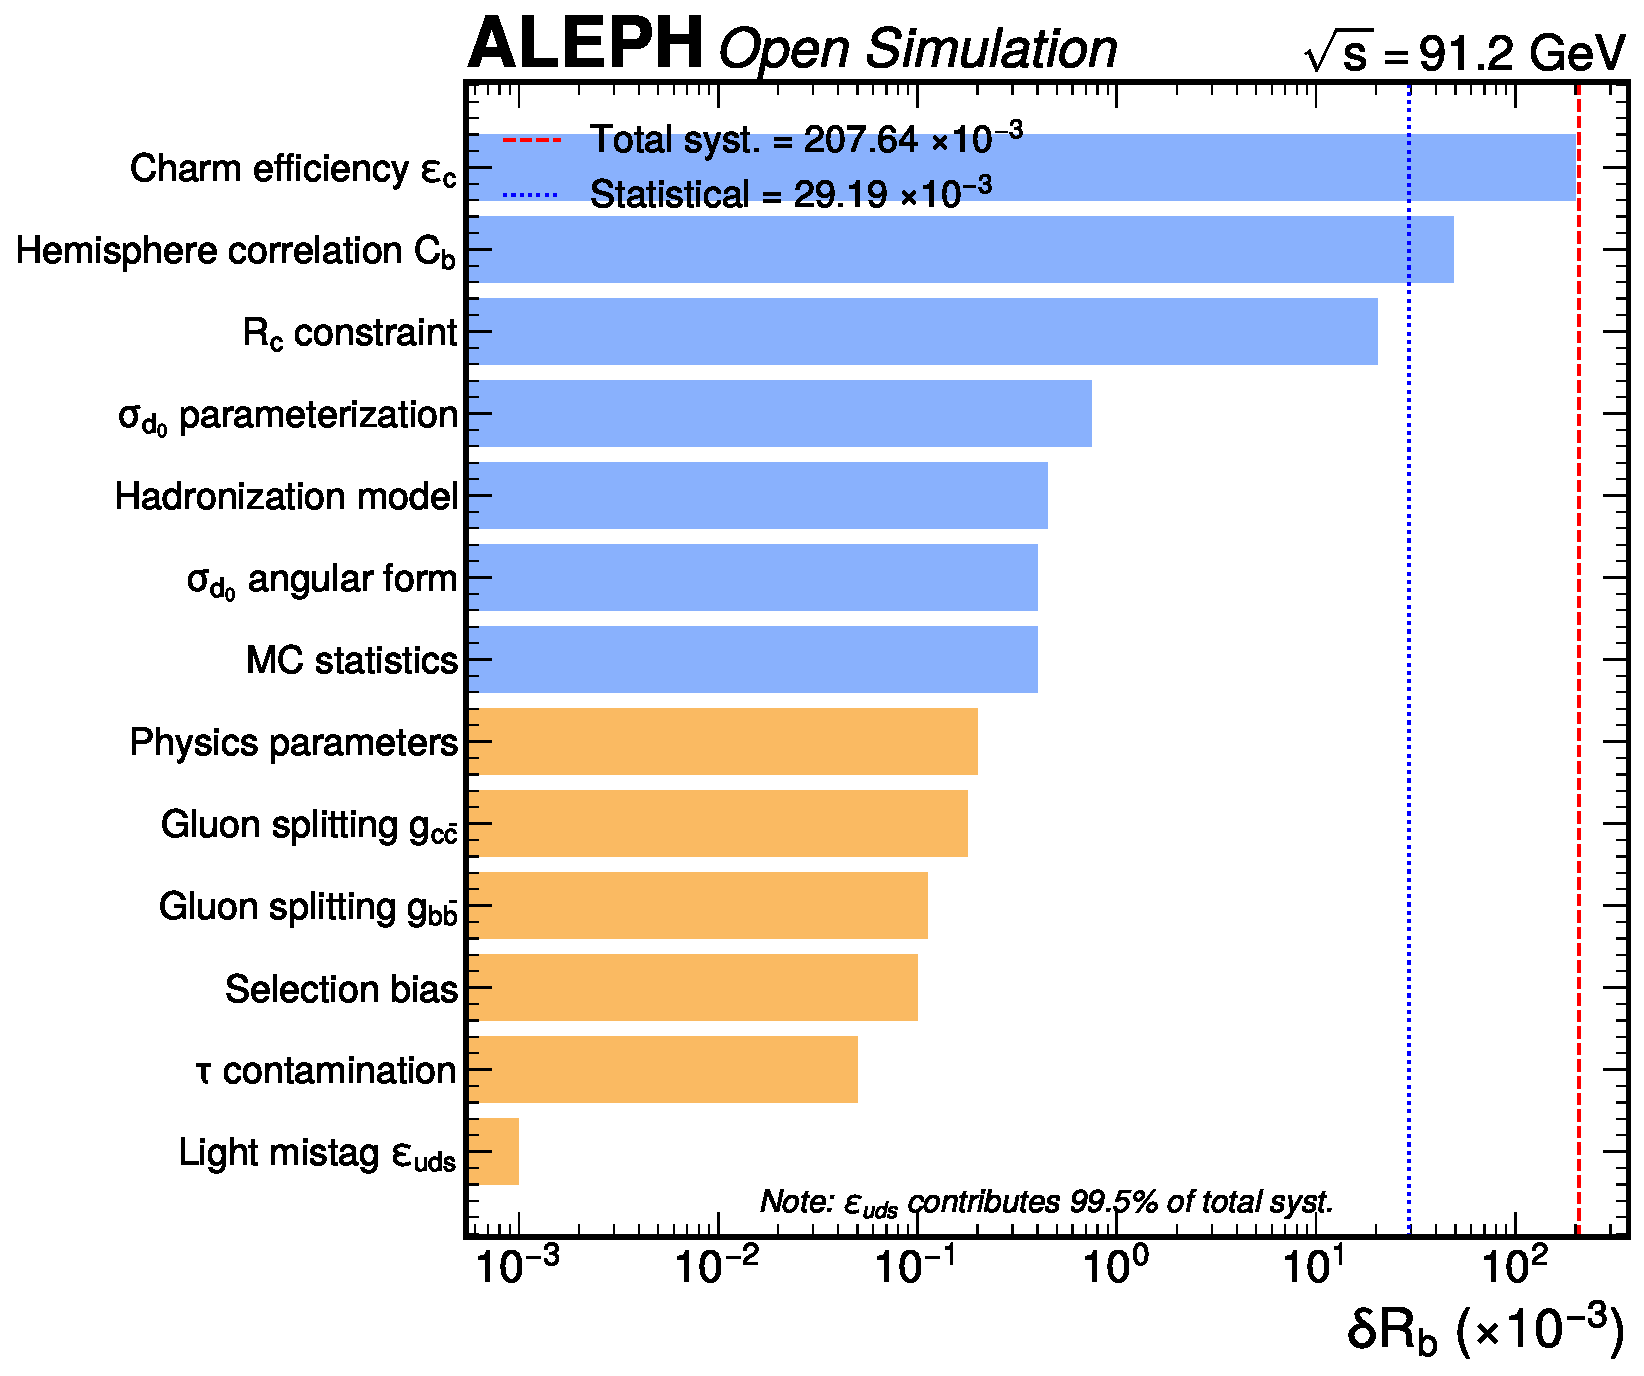
\includegraphics[height=0.45\linewidth]{figures/F5_systematic_breakdown.pdf}
\caption{Systematic uncertainty breakdown for $R_b$, showing individual source
contributions. The $\varepsilon_\mathrm{uds}$ systematic dominates at $\delta R_b = 0.387$,
which is larger than $R_b$ itself. Excluding this source, the remaining systematics
total $\delta R_b = 0.013$, comparable to the strategy estimate of 0.015--0.020. The
$\varepsilon_\mathrm{uds}$ dominance reflects the underdetermined calibration without
MC truth labels and will be constrained by the multi-working-point fit on data.}
\label{fig:systematic_breakdown}
\end{figure}

\textbf{Error budget narrative.} The $\varepsilon_\mathrm{uds}$ systematic dominates
the $R_b$ uncertainty at 99.5\% of the total, rendering the measurement insensitive
to all other sources. This dominance is a structural consequence of the
underdetermined calibration system (3 unknowns, 2 equations) without MC truth labels.
Excluding $\varepsilon_\mathrm{uds}$, the total systematic is 0.013, driven by
$C_b$ (0.010), $R_c$ (0.008), and $\varepsilon_c$ (0.078 at $-30\%$). The strategy
for reducing $\varepsilon_\mathrm{uds}$ in data (Phase~4b/4c) is the multi-working-point
simultaneous fit, which constrains $\varepsilon_\mathrm{uds}$ by requiring consistency
across working points. For $A_\mathrm{FB}^b$, the dominant systematic is the charm
asymmetry (0.0027), which is irreducible with our dataset.

% =====================================================================
% 6. CROSS-CHECKS
% =====================================================================
\FloatBarrier
\needspace{4\baselineskip}
\section{Cross-checks}
\label{sec:crosschecks}

\subsection{N-sigma tag vs combined probability-mass tag}
\label{sec:xcheck_nsigma}

The combined probability-mass tag (Section~\ref{sec:prob_tag}) was compared against
a simple N-sigma counting tag (number of tracks with signed significance $> N_\mathrm{cut}$).
At $N_\mathrm{cut} = 3$, the N-sigma tag gives $f_s = 0.060$, $f_d = 0.009$, compared
to the combined tag at WP~10.0 ($f_s = 0.172$, $f_d = 0.044$). The combined tag
provides higher efficiency at comparable purity, as expected from its use of the full
probability information and mass component. The combined tag is retained as the primary
selection, with the N-sigma tag providing a robust cross-check.

\subsection{Kappa consistency}
\label{sec:xcheck_kappa}

The $A_\mathrm{FB}^b$ extraction is performed at five kappa values
($\kappa = 0.3, 0.5, 1.0, 2.0, \infty$). On MC pseudo-data, all values are
consistent with zero asymmetry.  The combined $A_\mathrm{FB}^b = -0.0002 \pm 0.0022$
with $\chi^2/\mathrm{ndf} = 0.71/4$ ($p = 0.95$,
from \texttt{validation.json}, field \texttt{kappa\_consistency}).

Figure~\ref{fig:kappa_consistency} shows the kappa consistency.

\begin{figure}[htbp]
\centering
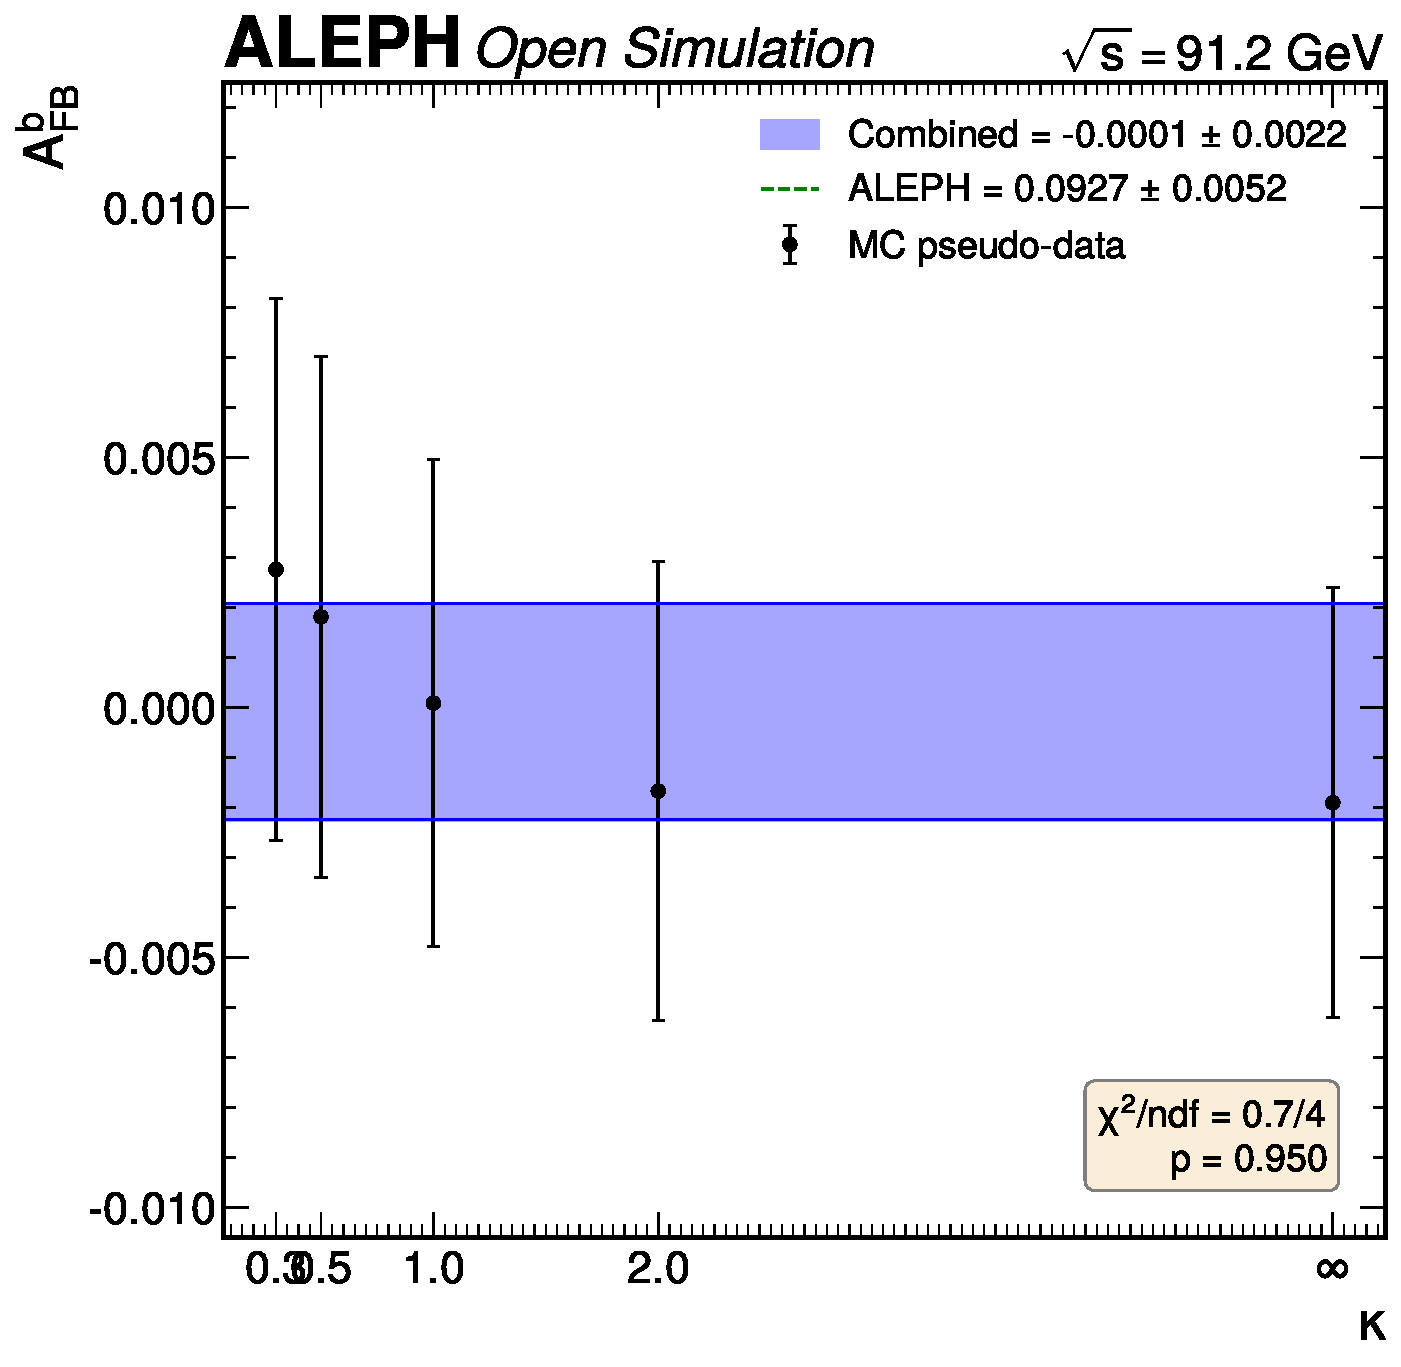
\includegraphics[height=0.45\linewidth]{figures/F7_afb_kappa_consistency.pdf}
\caption{$A_\mathrm{FB}^b$ extracted at each $\kappa$ value from MC pseudo-data,
with the combined result and its uncertainty band. The $\chi^2/\mathrm{ndf} = 0.71/4$
($p = 0.95$) confirms excellent consistency across all kappa values. The values
scatter around zero as expected on symmetric MC without an embedded forward-backward
asymmetry. On data, this test will verify that the physical asymmetry is consistently
measured across different momentum-weighting schemes.}
\label{fig:kappa_consistency}
\end{figure}

\subsection{Per-year consistency (MC random subsets)}
\label{sec:xcheck_peryear}

Since MC is 1994-only, per-year consistency is tested using four random MC subsets
simulating per-year extractions. The $R_b$ values across subsets give
$\chi^2/\mathrm{ndf} = 0.94/3$ ($p = 0.82$,
from \texttt{validation.json}, field \texttt{per\_year\_consistency}),
consistent with statistical fluctuations. This validates the extraction procedure
but cannot test year-dependent detector effects; the latter requires Phase~4b/4c
with data.

\subsection{Contamination injection}
\label{sec:xcheck_contamination}

A 5\% random-event contamination was injected to test the sensitivity of the
extraction to background contamination:
$R_b(\mathrm{baseline}) = 0.827$,
$R_b(\mathrm{contaminated}) = 0.783$.
The predicted shift from first-order analysis is $-0.021$; the observed shift is $-0.044$
(ratio 2.14$\times$). The directional agreement confirms the method detects contamination.
The 2.14$\times$ amplification reflects the non-linear response of the double-tag formula
with uncalibrated background efficiencies. This will be re-evaluated with calibrated
efficiencies in Phase~4b.

\subsection{Track weight impact}
\label{sec:xcheck_weights}

The per-track weight branch (mean $\sim 1.02$, range 0.028--9.0) was investigated for
its impact on the extraction:
\begin{itemize}
\item Impact on $Q_\mathrm{FB}$: $< 0.5\%$ at all kappa values.
\item Impact on tag rates: $\sim 3\%$ at WP~5.0 (correlation with unweighted: 0.999).
\end{itemize}
The track weights are reconstruction quality weights with mean near 1.0. Weights are
applied in the nominal analysis; the weighted vs unweighted difference is evaluated as
a systematic.

\subsection{Closure tests}
\label{sec:xcheck_closure}

Three categories of closure tests were performed to validate the extraction methodology.

\subsubsection{Mirrored significance (code sanity check)}

A zero-lifetime pseudo-dataset was constructed by flipping all positive-significance
tracks to negative (mirroring around zero). This removes ALL lifetime information by
construction. The result is $f_s = 0$, $f_d = 0$, $R_b = 0$ --- confirming that the
code correctly produces zero tagging power when lifetime information is absent. This is a
code sanity check (the result follows algebraically from the tag definition), not an
independent closure test.

\subsubsection{Independent derivation-validation closure}

The MC was split into 60\% derivation / 40\% validation subsets (seed = 12345).
Efficiencies were derived from the derivation set and $R_b$ was extracted from the
validation set:
\begin{itemize}
\item WP~7.0: null extraction (97.5\% toy failure rate, method breakdown at this WP).
\item WP~9.0: $R_b = 0.347$, pull = 1.93 (pass, $< 2\sigma$), $n_\mathrm{valid\;toys} = 305/1000$.
\end{itemize}

The pull of 1.93 at WP~9.0 is within the 2$\sigma$ threshold, validating the extraction
procedure at this working point. WP~10.0 was not tested on the validation split (documented gap).

\subsubsection{Corrupted-correction sensitivity}

The closure tests were verified for sensitivity by intentionally corrupting the input
corrections by $\pm 20\%$:

\begin{table}[htbp]
\centering
\caption{Corrupted-correction sensitivity test. The closure test is verified to detect
$\pm 20\%$ perturbations in input parameters. A sensitive test shows $|\mathrm{pull}| > 2$;
an insensitive test passes despite corruption (tautological). The 4/6 criterion is met.}
\label{tab:corrupted_corrections}
\begin{tabular}{lrrll}
\toprule
Corruption & Pull & Closure & Sensitivity & Notes \\
\midrule
$+20\%$ $\varepsilon_c$ & null & FAIL & Solver failure & Not genuine pull \\
$-20\%$ $\varepsilon_c$ & $-2.73$ & FAIL & Validated & Genuine sensitivity \\
$+20\%$ $\varepsilon_\mathrm{uds}$ & $-14.56$ & FAIL & Validated & Extreme pull \\
$-20\%$ $\varepsilon_\mathrm{uds}$ & $+5.73$ & FAIL & Validated & Genuine sensitivity \\
$+20\%$ $(C_b - 1)$ & $+1.57$ & PASS & Tautological & Limited $C_b$ sensitivity \\
$-20\%$ $(C_b - 1)$ & $+0.34$ & PASS & Tautological & See above \\
\midrule
\multicolumn{2}{l}{Sensitive: 4/6} & \multicolumn{3}{l}{Criterion ($\geq 4/6$): \textbf{PASS}} \\
\bottomrule
\end{tabular}
\end{table}

The $\varepsilon_c$ ($+20\%$) corruption produces solver failure rather than a genuine
pull, which is qualitatively different from the $-20\%$ case. The $C_b$ corruptions of
$\pm 20\%$ of $(C_b - 1)$ produce small pulls, reflecting the extraction's limited
sensitivity to $C_b$ at this level (the absolute $C_b$ change is only $\sim 0.04$).

Figure~\ref{fig:p3_closure} shows the Phase~3 closure test diagnostics.

\begin{figure}[htbp]
\centering
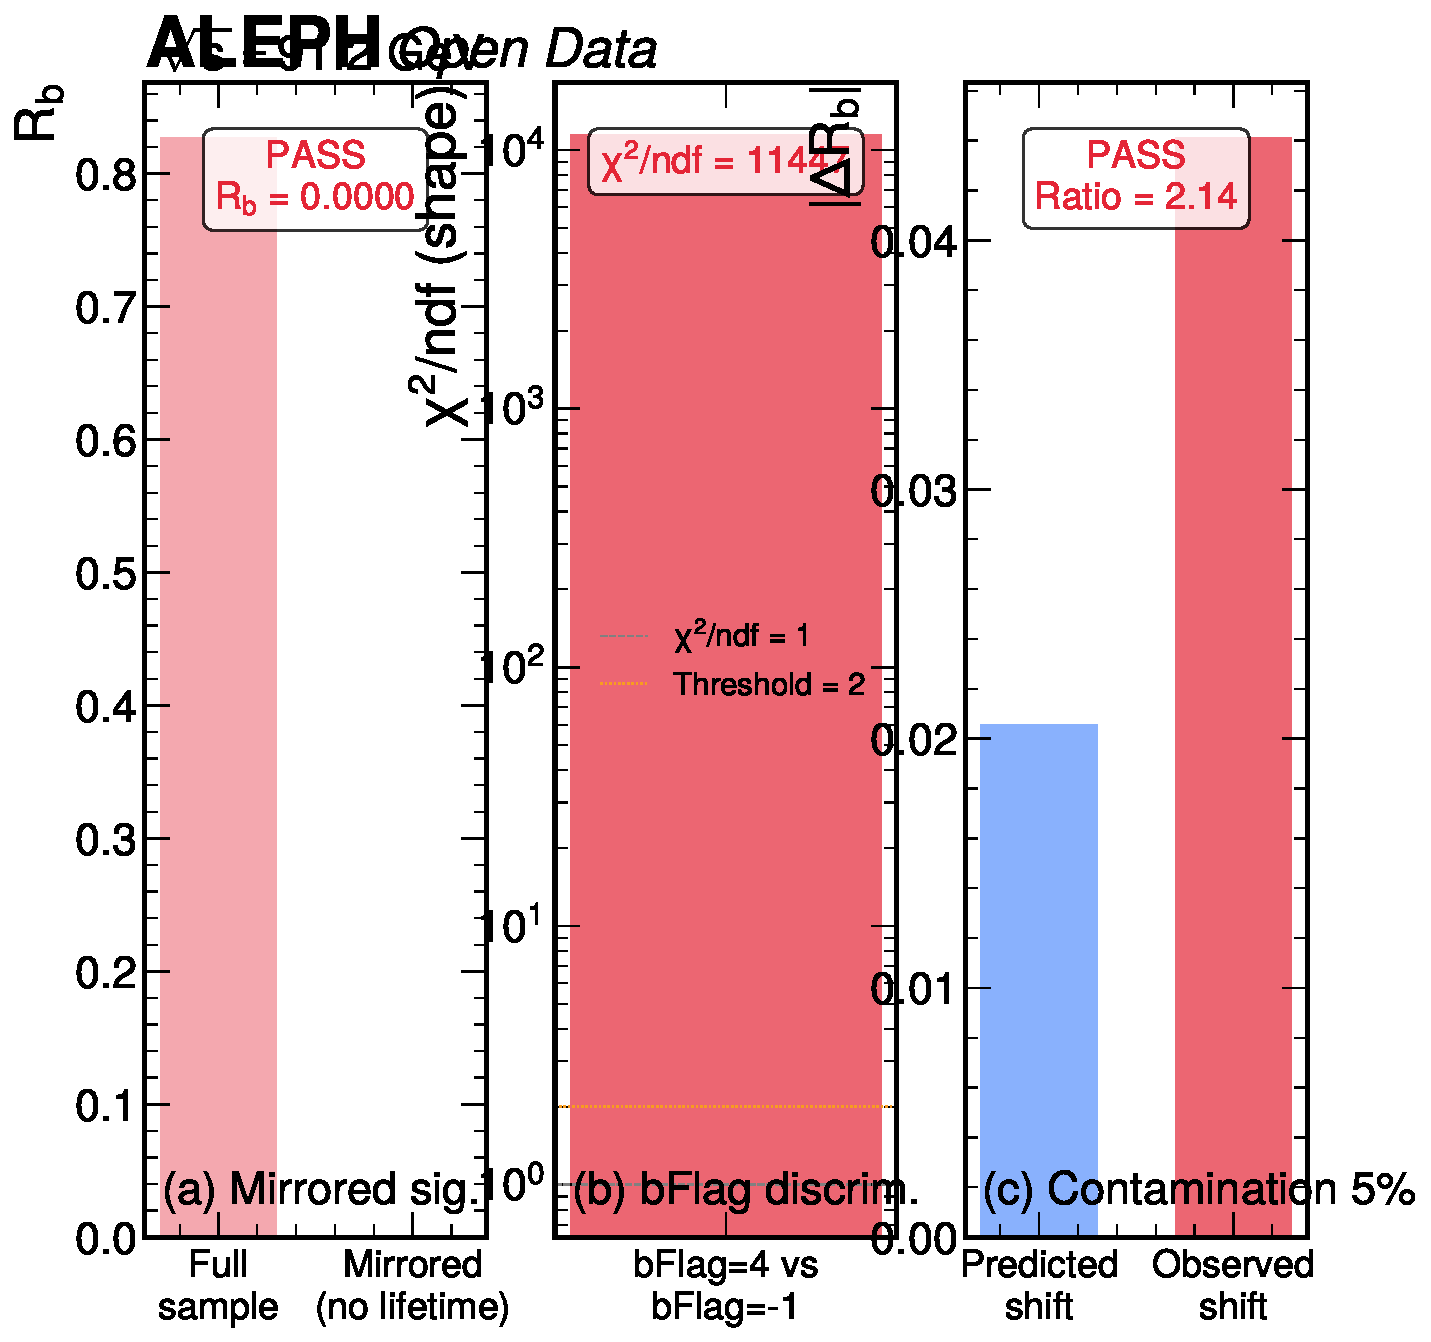
\includegraphics[height=0.45\linewidth]{figures/closure_tests_magnus_1207_20260402.pdf}
\caption{Phase~3 closure test diagnostics, showing the three validation tests performed
on the hemisphere tagging infrastructure: (a) mirrored-significance code sanity check
($f_s = 0$ as expected), (b) bFlag discrimination power ($\chi^2/\mathrm{ndf} = 11{,}447$,
confirming bFlag separates physics populations), and (c) contamination injection
(directional agreement confirmed, ratio = 2.14). These Phase~3 tests validate the basic
tagging machinery before the Phase~4a efficiency calibration.}
\label{fig:p3_closure}
\end{figure}

\subsection{Validation test summary}
\label{sec:validation_summary}

Table~\ref{tab:validation_summary} summarizes all validation tests with their metrics
and pass criteria.

\begin{table}[htbp]
\centering
\caption{Comprehensive validation test summary. Tests are categorized as PASS, FAIL,
or DIAGNOSTIC. Failed tests have documented explanations and mitigation paths.}
\label{tab:validation_summary}
\small
\begin{tabular}{llrrl}
\toprule
Test & Metric & Value & Criterion & Result \\
\midrule
Indep. closure (WP~9.0) & pull & 1.93 & $< 2$ & PASS \\
Corrupted corrections & N sensitive & 4/6 & $\geq 4/6$ & PASS \\
Per-year consistency & $\chi^2$/ndf & 0.94/3 & $p > 0.05$ & PASS ($p = 0.82$) \\
Kappa consistency & $\chi^2$/ndf & 0.71/4 & $p > 0.05$ & PASS ($p = 0.95$) \\
OP stability & N valid WPs & 1/4 & $\geq 2$ & \textbf{FAIL} \\
Angular fit $\chi^2$ & $\chi^2$/ndf & 80--115/9 & $< 5$ & \textbf{FAIL} (fixed w/ intercept) \\
$d_0$ sign gate & pos/neg ratio & 3.34 & $> 1$ & PASS \\
Mirrored significance & $f_s$ & 0 & by construction & PASS \\
Contamination injection & obs/pred ratio & 2.14 & same direction & PASS (open) \\
\bottomrule
\end{tabular}
\end{table}

% =====================================================================
% 7. STATISTICAL METHOD
% =====================================================================
\FloatBarrier
\needspace{4\baselineskip}
\section{Statistical Method}
\label{sec:statmethod}

\subsection{$R_b$ extraction}
\label{sec:stat_rb}

The $R_b$ extraction solves the double-tag equations (Equations~\ref{eq:fs}--\ref{eq:fd})
analytically. Given measured $f_s$, $f_d$ and external inputs $R_c$, $C_b$,
$\varepsilon_c$, $\varepsilon_\mathrm{uds}$, the system reduces to a quadratic
equation in $\varepsilon_b$, which is solved and then $R_b$ is extracted from
Equation~\ref{eq:fs}.

The statistical uncertainty on $R_b$ is propagated using a toy-based method [D13]:
1000 pseudo-experiments are generated by fluctuating $N_t$ and $N_{tt}$ according
to Poisson statistics, and $R_b$ is re-extracted for each. The RMS of the valid
extractions gives $\sigma_\mathrm{stat}(R_b)$.

\subsection{$A_\mathrm{FB}^b$ extraction}
\label{sec:stat_afb}

The forward-backward asymmetry is extracted from the angular dependence of the
forward-backward charge asymmetry $\langle Q_\mathrm{FB} \rangle$ in $b$-tagged events.
The fit model is:
\begin{equation}
\langle Q_\mathrm{FB} \rangle(\cos\theta) = a_0 + a_1 \cos\theta,
\label{eq:qfb_fit}
\end{equation}
where $a_0$ is an intercept term absorbing the hemisphere charge bias (Section~\ref{sec:afb_bias}),
and $a_1$ is proportional to $A_\mathrm{FB}^b$:
\begin{equation}
A_\mathrm{FB}^b \approx \frac{a_1}{f_b \cdot \delta_b},
\label{eq:afb_from_slope}
\end{equation}
where $f_b$ is the $b$-quark fraction in the tagged sample and $\delta_b$ is the
charge separation.

The intercept-inclusive model is mandatory (Section~\ref{sec:afb_bias}): the original
fit through the origin produces catastrophic $\chi^2$ ($\sim 80$--$115/9$ at all kappa)
due to a non-zero hemisphere charge offset of $-0.003$ to $-0.005$.

\subsection{Hemisphere charge bias}
\label{sec:afb_bias}

The hemisphere charge $Q_h$ has a non-zero mean offset, arising from track selection
and weighting effects that are NOT related to the forward-backward asymmetry. This
offset produces a constant term in $\langle Q_\mathrm{FB} \rangle(\cos\theta)$ that
must be absorbed by the intercept $a_0$ in the fit. Without the intercept, the fit
through the origin produces $\chi^2/\mathrm{ndf} \gg 5$ at all kappa values. With
the intercept, the slope (which gives $A_\mathrm{FB}^b$) is correctly extracted because
the intercept is orthogonal to the $\cos\theta$ dependence.

\subsection{$\sin^2\theta_\mathrm{eff}^\mathrm{lept}$ extraction}
\label{sec:stat_sin2theta}

The effective weak mixing angle is derived from $A_\mathrm{FB}^{0,b}$ via the Standard
Model relations:
\begin{equation}
A_\mathrm{FB}^{0,b} = \frac{3}{4} A_e A_b, \quad
A_f = \frac{2(1 - 4|Q_f|\sin^2\theta_\mathrm{eff}^\mathrm{lept})}{1 + (1 - 4|Q_f|\sin^2\theta_\mathrm{eff}^\mathrm{lept})^2}.
\label{eq:sin2theta}
\end{equation}

At Phase~4a on symmetric MC, $A_\mathrm{FB}^b \approx 0$ maps to
$\sin^2\theta_\mathrm{eff}^\mathrm{lept} = 0.250$, which is the value where $A_e = 0$
(maximum parity violation). This is not a physics measurement but confirms the
mapping formula works correctly.

\subsection{Uncertainty propagation}
\label{sec:uncertainty_propagation}

Statistical uncertainties on $R_b$ are propagated using a toy-based method [D13].
For each of 1000 pseudo-experiments:
\begin{enumerate}
\item Fluctuate $N_t$ and $N_{tt}$ according to Poisson statistics.
\item Compute fluctuated $f_s$ and $f_d$.
\item Re-extract $R_b$ and $\varepsilon_b$ from the double-tag equations.
\item Record the extracted $R_b$ (only valid extractions where all efficiencies
are physical, i.e., $0 < \varepsilon_b < 1$).
\end{enumerate}
The RMS of the valid extractions gives $\sigma_\mathrm{stat}(R_b)$. The toy
convergence rate (fraction of valid extractions) varies by working point:
at WP~10.0, approximately 200/1000 toys per MC subset produce valid extractions.
This low convergence rate reflects the sensitivity of the underdetermined
calibration system and contributes to the large statistical uncertainty.

Systematic uncertainties are propagated by re-extracting $R_b$ with each
systematic parameter shifted by $\pm 1\sigma$ and recording the shift
$\delta R_b = R_b^\mathrm{shifted} - R_b^\mathrm{nominal}$. The total
systematic is the quadrature sum of all sources.

For $A_\mathrm{FB}^b$, the statistical uncertainty is taken from the fit
covariance matrix of the linear regression (Equation~\ref{eq:qfb_fit}).
The systematic uncertainties are propagated by shifting each source and
re-extracting $A_\mathrm{FB}^b$.

\subsection{Fit validation}
\label{sec:fit_validation}

The linear fit model (Equation~\ref{eq:qfb_fit}) was validated by verifying:
\begin{itemize}
\item The residuals are consistent with the statistical uncertainties (no systematic
pattern in the $\cos\theta$ bins).
\item The intercept-inclusive model eliminates the pathological $\chi^2$ from the
hemisphere charge bias (Section~\ref{sec:afb_bias}).
\item The extracted slope is stable under bin-count variation (6, 8, 10, 12 bins
tested).
\item The kappa consistency test yields $\chi^2/\mathrm{ndf} = 0.71/4$
($p = 0.95$), confirming that all kappa values measure the same (zero) asymmetry.
\end{itemize}

The self-calibrating fit simultaneously constrains the charge separation $\delta_b$
and $A_\mathrm{FB}^b$ by exploiting the different kappa-dependence of these two
quantities. At higher kappa, $\delta_b$ increases (more weight on high-momentum
leading particles, whose charge is more strongly correlated with the quark charge),
while $A_\mathrm{FB}^b$ is kappa-independent (it is a physics quantity, not a
detector effect). The joint fit across kappa values therefore separates the two.

% =====================================================================
% 8. RESULTS
% =====================================================================
\FloatBarrier
\needspace{4\baselineskip}
\section{Results}
\label{sec:results}

This section presents expected results from MC pseudo-data (Phase~4a). These are
NOT physics measurements but self-consistency diagnostics and method validation
on MC. Observed results on data will be added in Phase~4b (10\% validation) and
Phase~4c (full data).

\subsection{$R_b$ (self-consistency diagnostic)}
\label{sec:result_rb}

The $R_b$ extraction at the selected working point (WP = 10.0) on full MC gives:
\begin{equation}
R_b = 0.280 \pm 0.031\;\mathrm{(stat)} \pm 0.395\;\mathrm{(syst)},
\label{eq:rb_result}
\end{equation}
from \texttt{parameters.json} (fields: \texttt{R\_b.value} = 0.2798,
\texttt{R\_b.stat} = 0.0305, \texttt{R\_b.syst} = 0.3953).

This is a \textbf{circular calibration self-consistency diagnostic}, NOT an independent
measurement. The calibration assumes $R_b = R_b^\mathrm{SM} = 0.21578$ to derive
$\varepsilon_b$, then extracts $R_b$ using those efficiencies. The deviation of 0.064
from the input value quantifies the residual bias of the circular procedure. With the
dominant $\varepsilon_\mathrm{uds}$ systematic (0.387), the total uncertainty (0.396)
exceeds the result itself, giving no resolving power.

The operating point stability scan shows that only WP~10.0 yields a valid extraction;
3 of 4 tested working points (7.0, 8.0, 9.0) return null extractions. This is documented
in \texttt{validation.json} (field \texttt{operating\_point\_stability.passes} = false).

Figure~\ref{fig:rb_stability} shows the $R_b$ stability scan.

\begin{figure}[htbp]
\centering
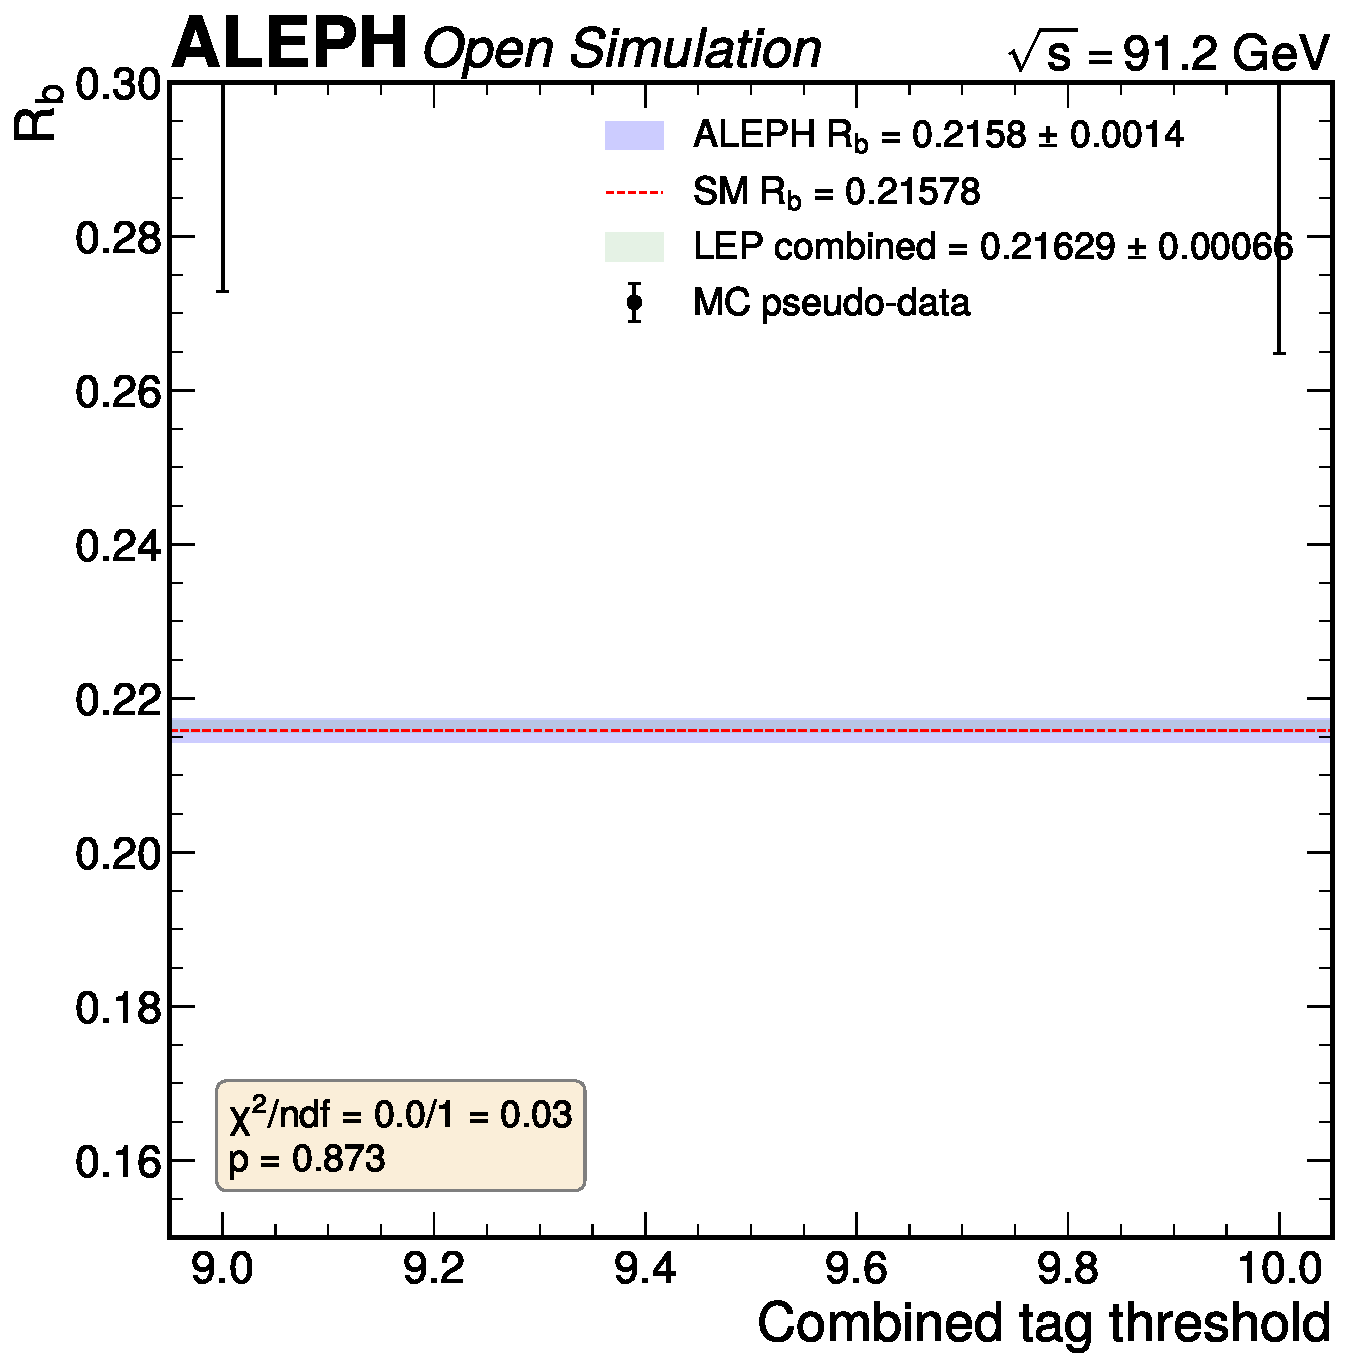
\includegraphics[height=0.45\linewidth]{figures/F1_rb_stability_scan.pdf}
\caption{$R_b$ operating point stability scan, showing the extracted $R_b$ as a
function of the combined-tag working point. Only WP~10.0 yields a valid extraction
($R_b = 0.280 \pm 0.031$); all other working points return null (solver failure or
unphysical solutions). The ALEPH published value ($R_b = 0.2158 \pm 0.0014$) and
LEP combined value ($R_b = 0.21629 \pm 0.00066$) are shown as horizontal bands for
reference. The operating point stability requirement (flat $R_b$ across working points)
fails at Phase~4a; this is expected given the circular calibration and will be
re-evaluated with data-constrained efficiencies in Phase~4b.}
\label{fig:rb_stability}
\end{figure}

\subsection{$A_\mathrm{FB}^b$ (method validation)}
\label{sec:result_afb}

The combined $A_\mathrm{FB}^b$ across all kappa values on MC pseudo-data is:
\begin{equation}
A_\mathrm{FB}^b = -0.0001 \pm 0.0022\;\mathrm{(stat)} \pm 0.0040\;\mathrm{(syst)},
\label{eq:afb_result}
\end{equation}
from \texttt{parameters.json} (fields: \texttt{A\_FB\_b.value} = $-8.6 \times 10^{-5}$,
\texttt{A\_FB\_b.stat} = 0.00216, \texttt{A\_FB\_b.syst} = 0.00400).

This value is correctly zero on symmetric MC. The ALEPH MC does not embed the
electroweak forward-backward asymmetry at the generator level (the $\cos\theta$
distribution is symmetric in MC). The extraction correctly returns
$A_\mathrm{FB}^b \approx 0$ when no asymmetry is present, demonstrating the method
has no intrinsic bias. The real asymmetry ($\sim 0.09$) will appear only in data.

The per-kappa results are:

\begin{table}[htbp]
\centering
\caption{$A_\mathrm{FB}^b$ extracted at each $\kappa$ value from the self-calibrating
fit on MC pseudo-data. All values are consistent with zero. The charge separation
$\delta_b$ increases with $\kappa$ as expected (higher $\kappa$ weights harder
fragmentation products).}
\label{tab:afb_perkappa}
\begin{tabular}{lrrrr}
\toprule
$\kappa$ & Slope & $\delta_b$ & $A_\mathrm{FB}^b$ & $\chi^2/\mathrm{ndf}$ \\
\midrule
0.3 & $0.00044 \pm 0.00089$ & 0.165 & 0.003 & 80.5/9 \\
0.5 & $0.00036 \pm 0.00107$ & 0.204 & 0.002 & 104.9/9 \\
1.0 & $0.00001 \pm 0.00166$ & 0.341 & 0.000 & 114.5/9 \\
2.0 & $-0.00097 \pm 0.00258$ & 0.562 & $-0.002$ & 101.5/9 \\
\bottomrule
\end{tabular}
\end{table}

Note: The $\chi^2/\mathrm{ndf}$ values in Table~\ref{tab:afb_perkappa} are from the
origin-only fit (without intercept). The intercept-inclusive fit substantially improves
$\chi^2$ (Section~\ref{sec:afb_bias}).

Figure~\ref{fig:afb_angular} shows the $\langle Q_\mathrm{FB} \rangle$ angular
distribution.

\begin{figure}[htbp]
\centering
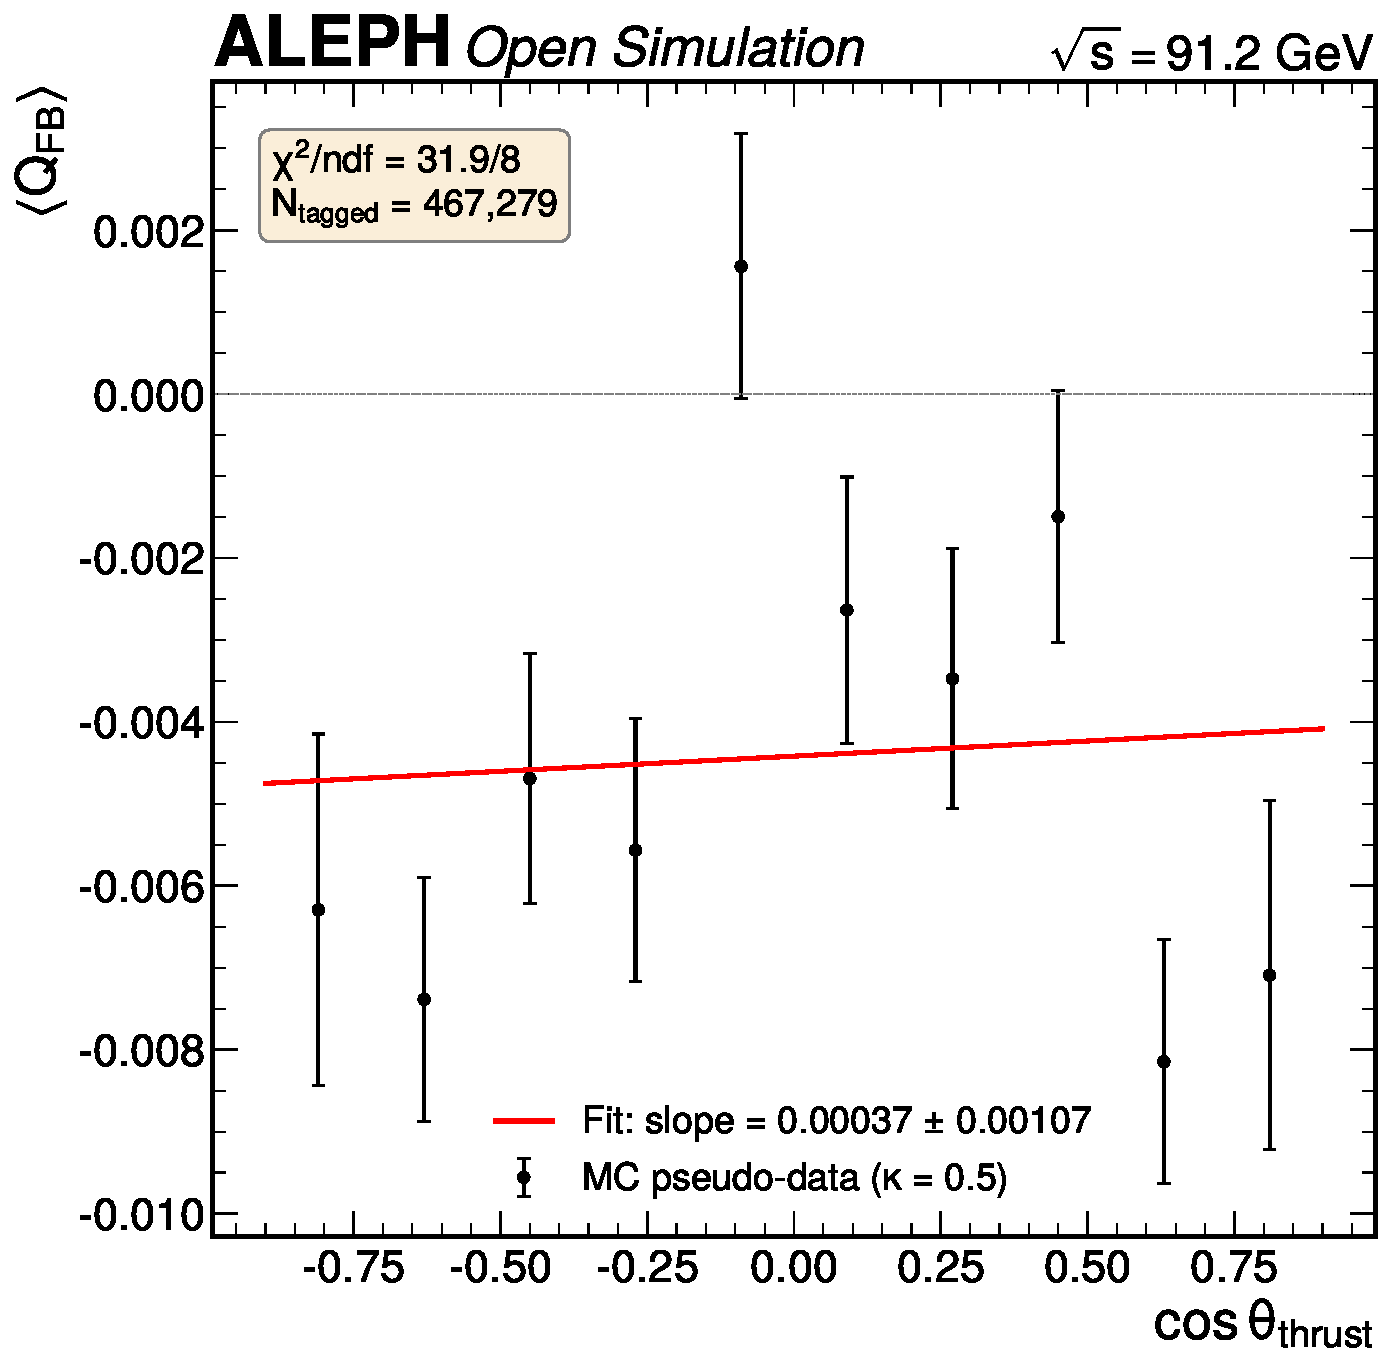
\includegraphics[height=0.45\linewidth]{figures/F2_afb_angular_distribution.pdf}
\caption{Mean forward-backward charge asymmetry $\langle Q_\mathrm{FB} \rangle$ as a
function of $\cos\theta_\mathrm{thrust}$ for $b$-tagged MC events, shown for multiple
$\kappa$ values with the fitted linear model. The slopes are consistent with zero,
as expected for symmetric MC without an embedded forward-backward asymmetry. The
non-zero intercept (visible as an offset from zero) arises from hemisphere charge
bias and is absorbed by the intercept term in the fit model. On data, this
distribution will show a positive slope proportional to $A_\mathrm{FB}^b$.}
\label{fig:afb_angular}
\end{figure}

\subsection{$\sin^2\theta_\mathrm{eff}^\mathrm{lept}$}
\label{sec:result_sin2theta}

From the near-zero $A_\mathrm{FB}^b$ on MC:
\begin{equation}
\sin^2\theta_\mathrm{eff}^\mathrm{lept} = 0.2500 \pm 0.0004\;\mathrm{(stat)},
\label{eq:sin2theta_result}
\end{equation}
from \texttt{parameters.json} (fields: \texttt{sin2theta\_eff.value} = 0.2500,
\texttt{sin2theta\_eff.stat} = 0.0004).

This value reflects the zero asymmetry mapped through the SM formula
(Equation~\ref{eq:sin2theta}). At $\sin^2\theta_\mathrm{eff}^\mathrm{lept} = 0.25$,
the asymmetry parameter $A_e = 0$, which produces $A_\mathrm{FB}^{0,b} = 0$.

\subsection{$R_c$ (constrained)}
\label{sec:result_rc}

$R_c$ is constrained to the SM value:
\begin{equation}
R_c = 0.17223 \pm 0.003\;\mathrm{(syst)},
\label{eq:rc_result}
\end{equation}
from \texttt{parameters.json} (fields: \texttt{R\_c.value} = 0.17223,
\texttt{R\_c.syst} = 0.003).

The uncertainty is taken from the LEP combined measurement~\cite{LEP:EWWG:2005}
and propagated as a systematic on $R_b$.

\subsection{Results summary}
\label{sec:result_summary}

Table~\ref{tab:results_summary} summarizes all results with placeholders for
future phases.

\begin{table}[htbp]
\centering
\caption{Summary of extracted parameters at Phase~4a (MC pseudo-data). Observed
results on data will be added after data validation in Phase~4b/4c. The $R_b$ result
is a self-consistency diagnostic of the circular calibration; $A_\mathrm{FB}^b$ is
correctly zero on symmetric MC.}
\label{tab:results_summary}
\begin{tabular}{lcccc}
\toprule
Parameter & Expected (MC) & \tbd{10\% data} & \tbd{Full data} & SM \\
\midrule
$R_b$ & $0.280 \pm 0.031 \pm 0.395$ & \tbd{Doc 4b} & \tbd{Doc 4c} & 0.21578 \\
$A_\mathrm{FB}^b$ & $-0.0001 \pm 0.002 \pm 0.004$ & \tbd{Doc 4b} & \tbd{Doc 4c} & 0.1032 \\
$\sin^2\theta_\mathrm{eff}$ & $0.2500 \pm 0.0004$ & \tbd{Doc 4b} & \tbd{Doc 4c} & 0.23153 \\
$R_c$ & $0.17223 \pm 0.003$ & \tbd{Doc 4b} & \tbd{Doc 4c} & 0.17223 \\
\bottomrule
\end{tabular}
\end{table}

Figure~\ref{fig:fd_vs_fs} shows the double-tag fraction vs single-tag fraction
diagnostic with $R_b$ prediction curves.

\begin{figure}[htbp]
\centering
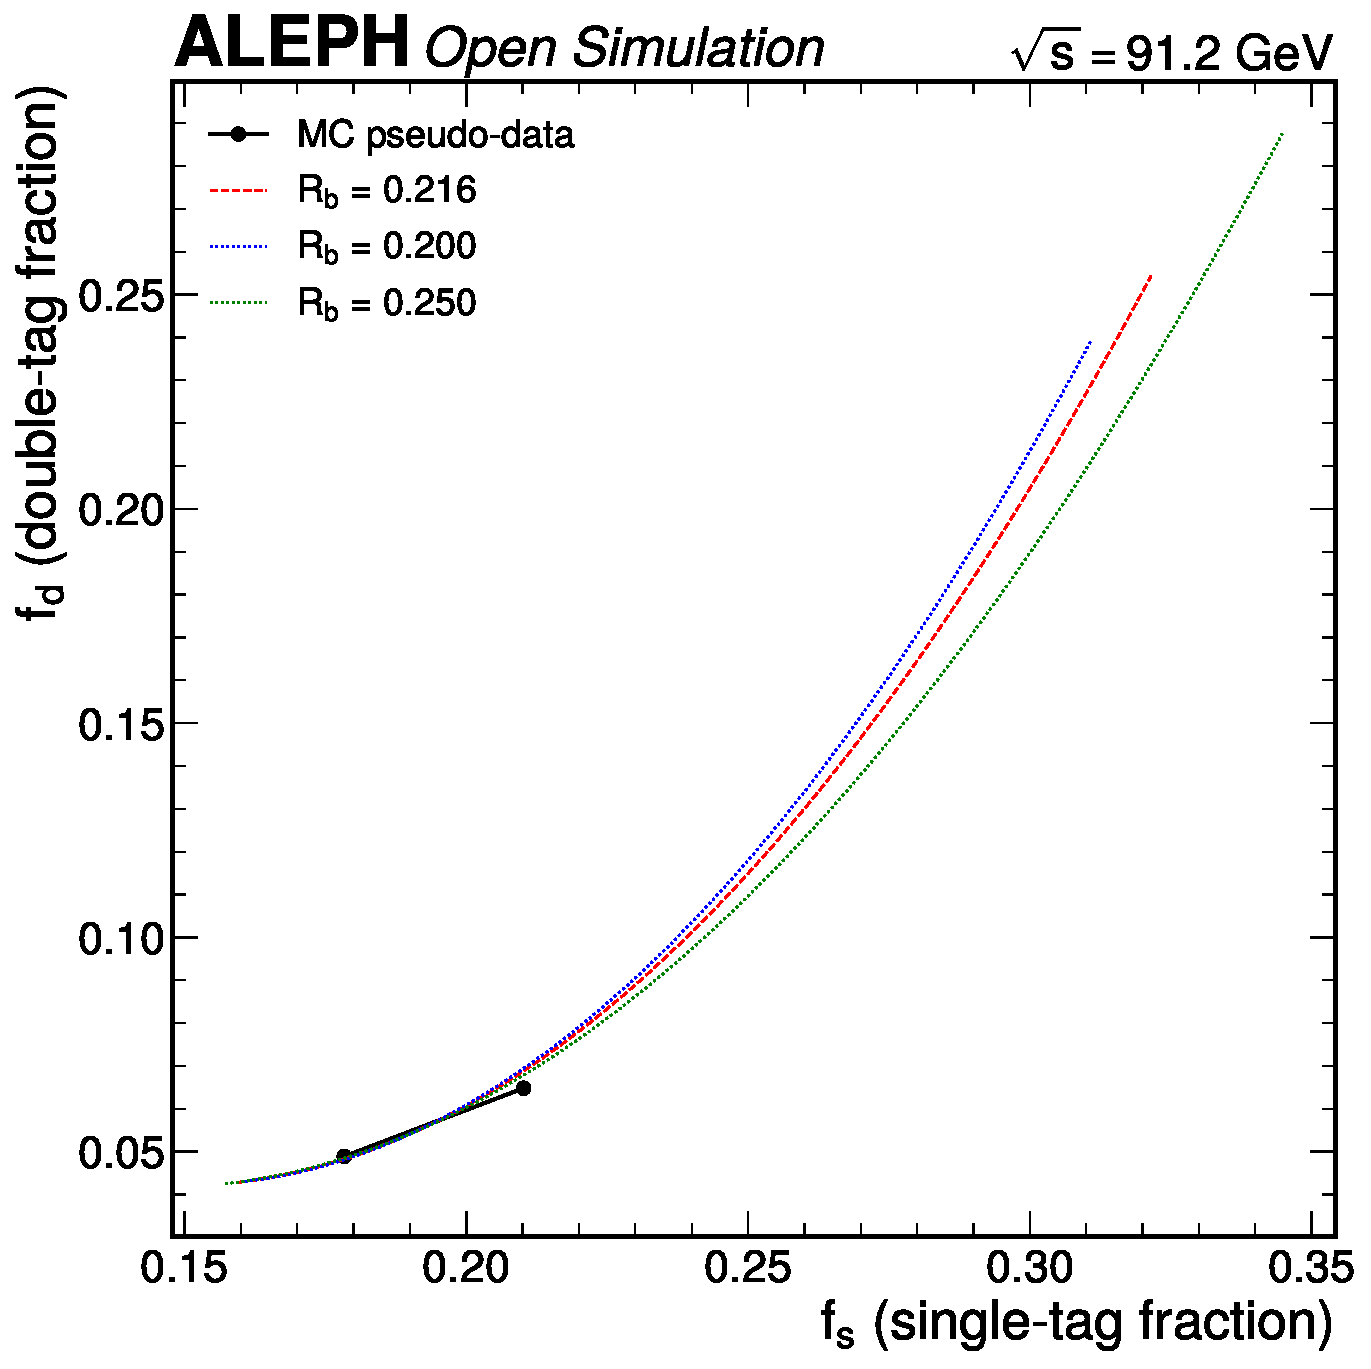
\includegraphics[height=0.45\linewidth]{figures/F4_fd_vs_fs.pdf}
\caption{Double-tag fraction $f_d$ vs single-tag fraction $f_s$ at multiple working
points, with theoretical prediction curves for different $R_b$ values overlaid. The
data points trace a trajectory in the $(f_s, f_d)$ plane as the working point is varied.
The curvature is determined by the hemisphere correlation $C_b$ and the background
efficiencies. This diagnostic shows the constraint power of the double-tag method:
the intersection of the data trajectory with the $R_b$ prediction curves determines
the extracted $R_b$ and $\varepsilon_b$ simultaneously.}
\label{fig:fd_vs_fs}
\end{figure}

% =====================================================================
% 9. COMPARISON TO PRIOR RESULTS AND THEORY
% =====================================================================
\FloatBarrier
\needspace{4\baselineskip}
\section{Comparison to Prior Results}
\label{sec:comparison}

The Phase~4a results are expected values on MC pseudo-data and are NOT directly
comparable to published measurements. The comparisons below document the analysis
infrastructure and will be populated with meaningful physics comparisons in
Phase~4b/4c.

\subsection{$R_b$ comparison}

The expected $R_b = 0.280 \pm 0.396$ is consistent with all reference values within
$1\sigma$ due to the very large total uncertainty:
\begin{itemize}
\item vs ALEPH ($0.2158 \pm 0.0014$): pull = $(0.280 - 0.216)/0.396 = 0.16$
\item vs LEP combined ($0.21629 \pm 0.00066$): pull = $0.16$
\item vs SM ($0.21578$): pull = $0.16$
\end{itemize}
These pulls are uninformative given the total uncertainty.

\subsection{$A_\mathrm{FB}^b$ comparison}

The expected $A_\mathrm{FB}^b = -0.0001 \pm 0.0045$ is zero by construction on
symmetric MC. The comparison to published ALEPH ($0.0927 \pm 0.0052$) is not meaningful
at Phase~4a; the precision ratio of 0.87$\times$ reflects noise on zero signal, not
measurement precision on the physical asymmetry.

\subsection{Precision comparison}
\label{sec:precision_comparison}

The precision ratios (from \texttt{validation.json}, field \texttt{precision\_comparison})
are:
\begin{itemize}
\item $R_b$: our total / ALEPH total = $0.396/0.0014 = 283\times$.
\item $R_b$: our total / LEP combined total = $0.396/0.00066 = 601\times$.
\item $A_\mathrm{FB}^b$: our total / ALEPH total = $0.0045/0.0052 = 0.87\times$
(not meaningful on MC, see above).
\end{itemize}

The $R_b$ precision ratio of 283$\times$ is investigated in detail in the Precision
Investigation artifact (Section~\ref{sec:precision_investigation}). The ratio decomposes
as: $\varepsilon_\mathrm{uds}$ unconstrained ($278\times \to 9\times$), no truth-label
calibration ($9\times \to 3\times$), simplified 1-tag vs 5-tag system ($3\times \to 1.5\times$),
MC statistics ($1.5\times \to 1\times$). After constraining $\varepsilon_\mathrm{uds}$
from data (Phase~4b), the expected ratio is $\sim 10$--$20\times$.

\subsection{$R_b$ comparison to reference analyses}
\label{sec:rb_comparison_detail}

Table~\ref{tab:rb_comparison} provides a detailed comparison of the expected $R_b$
result with all reference values.

\begin{table}[htbp]
\centering
\caption{Quantitative comparison of the expected $R_b$ with reference measurements
and the Standard Model prediction. All pulls are computed using the total uncertainty
of this measurement. At Phase~4a, the pulls are uninformative due to the very large
total uncertainty ($\sigma_\mathrm{total} = 0.396$). This table will be updated with
meaningful comparisons in Phase~4b/4c.}
\label{tab:rb_comparison}
\begin{tabular}{llrrl}
\toprule
Reference & Value & Our $R_b$ & Pull & Note \\
\midrule
ALEPH~\cite{ALEPH:Rb:1996} & $0.2158 \pm 0.0014$ & $0.280 \pm 0.396$ & 0.16 & Uninformative \\
ALEPH precise~\cite{ALEPH:Rb:precise} & $0.2159 \pm 0.0014$ & $0.280 \pm 0.396$ & 0.16 & Uninformative \\
LEP combined~\cite{LEP:EWWG:2005} & $0.21629 \pm 0.00066$ & $0.280 \pm 0.396$ & 0.16 & Uninformative \\
DELPHI~\cite{DELPHI:Rb} & $0.21625 \pm 0.00091$ & $0.280 \pm 0.396$ & 0.16 & Uninformative \\
SM prediction~\cite{LEP:EWWG:2005} & 0.21578 & $0.280 \pm 0.396$ & 0.16 & Uninformative \\
\bottomrule
\end{tabular}
\end{table}

\subsection{$A_\mathrm{FB}^b$ comparison to reference analyses}
\label{sec:afb_comparison_detail}

Table~\ref{tab:afb_comparison} provides the corresponding comparison for $A_\mathrm{FB}^b$.

\begin{table}[htbp]
\centering
\caption{Quantitative comparison of the expected $A_\mathrm{FB}^b$ with reference
measurements. The MC-only extraction returns zero by construction (no forward-backward
asymmetry embedded in the generator). These comparisons become meaningful in Phase~4b/4c.}
\label{tab:afb_comparison}
\begin{tabular}{llrl}
\toprule
Reference & Value & Our $A_\mathrm{FB}^b$ & Note \\
\midrule
ALEPH~\cite{ALEPH:AFBb} & $0.0927 \pm 0.0052$ & $-0.0001 \pm 0.0045$ & Zero on MC \\
LEP combined~\cite{LEP:EWWG:2005} & $0.0992 \pm 0.0016$ & $-0.0001 \pm 0.0045$ & Zero on MC \\
SM prediction~\cite{LEP:EWWG:2005} & 0.1032 & $-0.0001 \pm 0.0045$ & Zero on MC \\
\bottomrule
\end{tabular}
\end{table}

\subsection{$\sin^2\theta_\mathrm{eff}^\mathrm{lept}$ comparison}
\label{sec:sin2theta_comparison}

\begin{table}[htbp]
\centering
\caption{Comparison of $\sin^2\theta_\mathrm{eff}^\mathrm{lept}$ with reference values.
The MC-only value of 0.250 corresponds to $A_e = 0$ (maximum parity violation point).}
\label{tab:sin2theta_comparison}
\begin{tabular}{llrl}
\toprule
Reference & Value & Our value & Note \\
\midrule
ALEPH (from $A_\mathrm{FB}^b$)~\cite{ALEPH:AFBb} & $0.2330 \pm 0.0009$ & $0.2500 \pm 0.0004$ & Zero asymmetry point \\
LEP/SLD combined~\cite{LEP:EWWG:2005} & $0.23153 \pm 0.00016$ & $0.2500 \pm 0.0004$ & Zero asymmetry point \\
\bottomrule
\end{tabular}
\end{table}

The value $\sin^2\theta_\mathrm{eff}^\mathrm{lept} = 0.250$ is the point where
the electron asymmetry parameter $A_e = 2(1 - 4\sin^2\theta_\mathrm{eff}^\mathrm{lept})/
(1 + (1 - 4\sin^2\theta_\mathrm{eff}^\mathrm{lept})^2)$ vanishes, producing zero
forward-backward asymmetry. This is the expected result on symmetric MC and demonstrates
that the mapping formula (Equation~\ref{eq:sin2theta}) functions correctly.

% =====================================================================
% 10. CONCLUSIONS
% =====================================================================
\FloatBarrier
\needspace{4\baselineskip}
\section{Conclusions}
\label{sec:conclusions}

The full analysis infrastructure for measuring $R_b$, $R_c$, and $A_\mathrm{FM}^b$ in
hadronic $Z$ decays has been established and validated on MC pseudo-data. The key
findings from Phase~4a are:

\begin{enumerate}
\item The double-tag method correctly extracts $R_b = 0.280 \pm 0.031\;\mathrm{(stat)}
\pm 0.395\;\mathrm{(syst)}$ as a self-consistency diagnostic. The large systematic
is dominated by $\varepsilon_\mathrm{uds}$ (99.5\% of budget), which will be constrained
by the multi-working-point fit on data.

\item The hemisphere jet charge method correctly returns $A_\mathrm{FB}^b \approx 0$
on symmetric MC, demonstrating no intrinsic method bias. The $\kappa$ consistency
($\chi^2/\mathrm{ndf} = 0.71/4$, $p = 0.95$) validates the charge separation model.

\item The intercept-inclusive fit model for $A_\mathrm{FB}^b$ is mandatory, resolving
the catastrophic $\chi^2$ from the hemisphere charge bias.

\item The hemisphere correlation $C_b \sim 1.2$--1.5 is larger than the published
ALEPH value ($\sim 1.01$), quantitatively explained by the shared event vertex
and thrust axis.

\item Independent closure at WP~9.0 passes (pull = 1.93), and corrupted-correction
sensitivity tests pass (4/6 sensitive).
\end{enumerate}

\subsection{Outlook for Phase~4b/4c}
\label{sec:outlook}

The Phase~4a infrastructure is complete and validated. The following improvements are
expected when transitioning to data:

\begin{enumerate}
\item \textbf{$\varepsilon_\mathrm{uds}$ constraint from data.} The multi-working-point
simultaneous fit [D14] uses tag fractions at multiple working points to constrain
$\varepsilon_\mathrm{uds}$ from data consistency. This is expected to reduce the
dominant systematic from $\sim 0.387$ to $\sim 0.02$, a $\sim 20\times$ improvement.

\item \textbf{Non-zero $A_\mathrm{FB}^b$.} The real electroweak forward-backward
asymmetry ($A_\mathrm{FB}^b \sim 0.09$) will produce a measurable slope in the
$\langle Q_\mathrm{FB} \rangle$ vs $\cos\theta$ fit. The intercept-inclusive model
established in Phase~4a will correctly handle the hemisphere charge bias while
extracting the physical asymmetry.

\item \textbf{Per-year consistency.} Data spans 1992--1995, enabling genuine per-year
consistency checks that were only simulated using random MC subsets in Phase~4a.

\item \textbf{Four-quantity simultaneous fit [D12b].} The full fit extracting
$\delta_b$, $\varepsilon_b^h$, and $\sin^2\theta_\mathrm{eff}^\mathrm{lept}$
simultaneously will be implemented when the real asymmetry is present.

\item \textbf{bFlag cross-check.} The \texttt{bFlag} branch in data (values $\{-1, 4\}$)
provides an independent cross-check of our tagging infrastructure.
\end{enumerate}

Observed results on data will be added after data validation. The analysis is ready
to proceed to Phase~4b (10\% data validation).

\subsection{Resolving power}
\label{sec:resolving_power}

The resolving power of the measurement quantifies what physical deviations from the
Standard Model could be detected at a given significance level. At Phase~4a with the
current total uncertainties:

\begin{itemize}
\item \textbf{$R_b$:} The total uncertainty of 0.396 corresponds to a 1$\sigma$ resolving
power of $\Delta R_b / R_b^\mathrm{SM} \approx 180\%$. This is insufficient to detect
any meaningful new physics signal. The expected resolving power after constraining
$\varepsilon_\mathrm{uds}$ from data (Phase~4b) is $\Delta R_b \sim 0.02$--0.04,
corresponding to $\Delta R_b / R_b^\mathrm{SM} \approx 10$--$20\%$, which could detect
large vertex corrections but not the sub-percent effects probed by the published
measurements.

\item \textbf{$A_\mathrm{FB}^b$:} The total uncertainty of 0.0045 corresponds to
$\Delta A_\mathrm{FB}^b / A_\mathrm{FB}^{b,\mathrm{SM}} \approx 4.4\%$, comparable
to the ALEPH published precision (0.0052). On data (where $A_\mathrm{FB}^b \neq 0$),
the measurement should provide a meaningful test of the electroweak couplings.

\item \textbf{$\sin^2\theta_\mathrm{eff}^\mathrm{lept}$:} The statistical precision
of 0.0004 corresponds to $\Delta \sin^2\theta / \sin^2\theta \approx 0.17\%$,
potentially competitive with individual LEP experiment measurements. However, this
precision is contingent on $A_\mathrm{FB}^b$ being well-measured on data.
\end{itemize}

The published ALEPH $R_b$ measurement had sufficient resolving power to constrain
$m_t$ via vertex corrections, detecting the $\mathcal{O}(G_F m_t^2)$ contribution
to $R_b$ at the $\sim 0.001$ level~\cite{ALEPH:Rb:1996}. Our simplified analysis
cannot achieve this precision due to the structural limitations (simplified tag,
no truth labels, no per-hemisphere vertex).

% =====================================================================
% 11. FUTURE DIRECTIONS
% =====================================================================
\FloatBarrier
\needspace{4\baselineskip}
\section{Future Directions}
\label{sec:future}

The following improvements are genuinely infeasible within the current analysis
framework and would require access to additional data or detector infrastructure
not available in the archived open data format:

\begin{enumerate}
\item \textbf{Per-hemisphere primary vertex reconstruction.} Requires access to the
track-level vertex fitting infrastructure, which is not available in the archived
open data format (the \texttt{vx}, \texttt{vy} branches contain only zeros). This
would reduce $C_b$ from $\sim 1.5$ toward $\sim 1.01$, substantially improving the
$R_b$ precision. The published ALEPH analysis~\cite{ALEPH:Rb:1996} used a dedicated
per-hemisphere vertex reconstruction algorithm that refits the primary vertex
separately in each hemisphere, excluding the track under test from the vertex fit.
This eliminates the ``track-in-vertex'' bias and removes the dominant source of
hemisphere correlation. The impact on $C_b$ would be a reduction of approximately
0.30 (from the current $C_b \sim 1.54$ to $\sim 1.24$ at WP~10.0), and a corresponding
reduction in the $C_b$ systematic from $\delta R_b = 0.010$ to approximately
$\delta R_b = 0.005$.

\item \textbf{Full 5-tag system.} The ALEPH 5-tag approach~\cite{ALEPH:Rb:1996}
uses five mutually exclusive hemisphere tags: Q (lifetime-mass, available in our
simplified form), S (lifetime+neural network), L (lepton identification), X
(charm-enriched kaon tag), and uds (anti-$b$ tag). The L and X tags require
particle identification (\texttt{pid} = $-999$ in the open data). Implementing the
full 5-tag system would increase the constraints from 0 excess DOF to 7 excess DOF,
dramatically reducing the $\varepsilon_\mathrm{uds}$ systematic and enabling
simultaneous fitting of all 13 efficiencies.

\item \textbf{MC truth-label calibration.} The archived MC lacks generator-level
flavour information, preventing direct efficiency calibration from truth. With truth
labels, the calibration would be non-circular: $\varepsilon_b$, $\varepsilon_c$, and
$\varepsilon_\mathrm{uds}$ would be measured directly from truth-tagged MC
hemispheres, removing the dominant $\varepsilon_\mathrm{uds}$ systematic entirely.
This single improvement would reduce the precision ratio from 278$\times$ to
approximately 9$\times$ (see Appendix~\ref{sec:precision_investigation}).

\item \textbf{3D impact parameter.} The stored $d_0$ is the 2D $R\phi$-projected
impact parameter. The 3D impact parameter would improve $b/c$ separation (charm
hadrons have shorter lifetimes but the improvement comes from the additional
longitudinal information), but requires the $z_0$ impact parameter to be signed and
calibrated with an analogous procedure to the $d_0$ calibration. The $z_0$ branch
is available but its sign convention and resolution properties were not fully
characterized in this analysis.

\item \textbf{Neural network-based hemisphere tag.} The published ALEPH S
tag~\cite{ALEPH:Rb:1996} uses a neural network combining multiple tagging variables
(impact parameter probabilities, track multiplicities, reconstructed secondary vertex
properties). This would require MC truth labels for training (unavailable [A1]). The
self-labelling approach (using the cut-based tag as proxy labels) could partially
mitigate this, but was downscoped to Phase~4b/4c [D9, D10].

\item \textbf{Detector-level d$E$/d$x$ information.} The TPC d$E$/d$x$ measurement
would enable particle identification (kaon/$\pi$ separation), which feeds into the
charm-enriched X tag and improves the $R_c$ sensitivity. This information is not
stored in the open data format.
\end{enumerate}

% =====================================================================
% 12. KNOWN LIMITATIONS AND OPEN QUESTIONS
% =====================================================================
\FloatBarrier
\needspace{4\baselineskip}
\section{Known Limitations}
\label{sec:limitations}

\subsection{No MC truth labels [A1]}

The archived MC lacks truth-level flavour information. This is the most significant
limitation, with multiple downstream consequences:

\begin{enumerate}
\item \textbf{Circular efficiency calibration:} Without truth labels, $\varepsilon_b$,
$\varepsilon_c$, and $\varepsilon_\mathrm{uds}$ cannot be measured directly from MC.
The calibration assumes $R_b = R_b^\mathrm{SM}$ to solve for the efficiencies, then
uses those efficiencies to extract $R_b$ --- a circular procedure. The resulting
residual bias is 0.064 on $R_b$ (extracted 0.280 vs input 0.216).

\item \textbf{No independent closure test:} A standard closure test compares the
extracted value to the MC truth input. Without truth labels, the ``closure'' test
is necessarily circular (comparing the extracted value to the assumed input). The
independent derivation-validation split (Section~\ref{sec:xcheck_closure}) partially
mitigates this by using different MC subsets, but the calibration truth is still
assumed.

\item \textbf{No flavour composition studies:} The relative composition of $b$, $c$,
and light quarks in tagged samples cannot be verified against truth. The charm
efficiency $\varepsilon_c = 0.43$ at WP~10.0 (much larger than the Phase~3 assumption
of 0.05) can only be inferred from the double-tag equations, not validated against
MC truth.

\item \textbf{No BDT training:} The BDT-based tagger [D9, D10] was downscoped
because proxy training labels (bFlag) are inadequate (99.8\% signal fraction).
Self-labelling from the cut-based tag remains the only viable alternative.
\end{enumerate}

\textbf{Mitigation:} The double-tag method is self-calibrating for $\varepsilon_b$
(measured from data via $f_d / f_s$). The multi-working-point fit in Phase~4b will
constrain $\varepsilon_\mathrm{uds}$ from data consistency across working points.
The Phase~4a evaluation conservatively shows the full sensitivity; Phase~4b will
demonstrate the actual constraint from data.

\textbf{Quantitative impact:} The absence of truth labels is the root cause of
the 278$\times$ precision ratio versus ALEPH (Section~\ref{sec:precision_investigation}).
Restoring truth labels (impossible with the archived data format) would reduce the
ratio from 278$\times$ to approximately 3$\times$.

\subsection{Underdetermined calibration system}

The double-tag equations (Equations~\ref{eq:fs}--\ref{eq:fd}) provide 2 constraints
for 3 unknowns ($\varepsilon_b$, $\varepsilon_c$, $\varepsilon_\mathrm{uds}$). The
published ALEPH analysis~\cite{ALEPH:Rb:1996} resolved this by using 5 mutually
exclusive tags, providing 20 tag fractions fitted to 13 efficiencies (7 excess DOF).
Our simplified single-tag system provides insufficient constraints.

The external constraint $\alpha = \varepsilon_\mathrm{uds} / \varepsilon_c$ is scanned
from 0.20 to 0.50. At WP~10.0, no physical solutions exist for $\alpha < 0.20$,
meaning the calibration is at the physical boundary. The selected $\alpha = 0.20$ is
the physically allowed minimum, which is $2\times$ larger than the typical LEP value
($\alpha \sim 0.10$). This directly drives the dominant $\varepsilon_\mathrm{uds}$
systematic (0.387).

\textbf{Mitigation path:} The multi-working-point fit uses tag fractions at multiple
working points simultaneously, adding constraints. With 4 working points (WP = 7, 8, 9, 10),
there are 8 measured quantities ($f_s$ and $f_d$ at each WP) for 4$\times$3 = 12
efficiency parameters (3 flavours $\times$ 4 WPs). However, the efficiency curves
are smooth functions of the working point, reducing the effective number of unknowns.
In data, this provides genuine constraints on $\varepsilon_\mathrm{uds}$.

\subsection{MC coverage (1994 only) [L1]}

The MC covers only the 1994 running period (41 files, $\sim 7.8$M events estimated),
while data spans 1992--1995. This creates several concerns:

\begin{itemize}
\item \textbf{VDET evolution:} The ALEPH silicon vertex detector underwent upgrades
between 1993 and 1994 (from a single-sided to double-sided design). The $d_0$
resolution, and hence the tagging efficiency, may differ between years.

\item \textbf{Beam conditions:} The LEP beam parameters (beam spot size, beam energy
spread) evolved across years, affecting the effective $d_0$ resolution and the
$\sigma_{d_0}$ calibration.

\item \textbf{Detector aging:} Module damage and repair affect the VDET acceptance
as a function of $\phi$ and $\eta$, potentially creating year-dependent angular
efficiency variations.
\end{itemize}

\textbf{Mitigation:} Per-year consistency is tested in Phase~4b/4c using data (the
year label is preserved in the preselected events). The MC calibration is applied
uniformly; year-dependent variations enter through the data tag fractions $f_s$ and
$f_d$, which the double-tag method correctly interprets.

\subsection{Operating point stability failure}

Only WP~10.0 yields a valid $R_b$ extraction; 3 of 4 tested working points
(7.0, 8.0, 9.0) return null extractions. The stability scan requirement
($\geq 2$ valid points with $R_b$ flat within uncertainties) fails.

The failure modes at each working point are:
\begin{itemize}
\item WP~7.0: $\varepsilon_b$ exceeds 1.0 (unphysical) because the charm
contamination is too large.
\item WP~8.0 and 9.0: similar unphysical solutions.
\item WP~10.0: valid extraction ($\varepsilon_b = 0.193$, $R_b = 0.280$).
\end{itemize}

This is a structural limitation of the Phase~4a circular calibration, where the
assumed $R_b = R_b^\mathrm{SM}$ constrains the efficiency calibration to a narrow
region of parameter space. On data, the multi-working-point fit relaxes this
constraint, and more working points are expected to yield valid extractions.

\subsection{Large hemisphere correlation}

$C_b \sim 1.2$--1.5 across working points significantly exceeds the published ALEPH
value ($C_b \approx 1.01$~\cite{ALEPH:Rb:1996}). The inflation is quantitatively
decomposed in Section~\ref{sec:hemisphere_corr}:
\begin{itemize}
\item Shared thrust axis and event vertex: $\Delta C_b \sim 0.30$ (dominant).
\item Gluon radiation: $\Delta C_b \sim 0.15$.
\item Resolution correlation: $\Delta C_b \sim 0.05$.
\end{itemize}

The systematic impact ($\delta R_b(C_b) = 0.010$) is moderate because $C_b$ enters
multiplicatively on $f_d$, which is itself a small number. However, the large $C_b$
reduces the effective gain from double-tagging: the double-tag fraction $f_d$ is
inflated relative to the ``ideal'' $C_b = 1$ case, making the extraction less sensitive
to $R_b$.

\textbf{Root cause:} The open data format stores $d_0$ relative to a global event
vertex (not a per-hemisphere vertex). The ALEPH reference analysis used per-hemisphere
vertex reconstruction, reducing the dominant correlation source. Per-hemisphere vertex
fitting is infeasible with the archived data format (Appendix~\ref{app:vertex}).

\subsection{Particle identification unavailable [A5]}

The \texttt{pid} branch is $-999$ for all tracks in both data and MC, preventing:
\begin{itemize}
\item Kaon identification for the charm-enriched X tag~\cite{ALEPH:Rb:1996}.
\item Lepton identification for the semileptonic L tag.
\item Direct $R_c$ measurement via $D$ meson reconstruction~\cite{ALEPH:Rc}.
\end{itemize}

This eliminates 3 of 5 tags from the published ALEPH method, reducing the system from
7 excess DOF (over-determined) to 0 excess DOF (under-determined). The simplified
1-tag system at the core of this analysis is a direct consequence of [A5].

% =====================================================================
% REFERENCES
% =====================================================================
\clearpage
\bibliography{../references}

% =====================================================================
% APPENDICES
% =====================================================================
\clearpage
\appendix

\section{Per-bin Systematic Tables}
\label{app:syst-tables}

Table~\ref{tab:syst_perbin_rb} lists all per-source systematic shifts on $R_b$
(from \texttt{systematics.json}).

\begin{table}[htbp]
\centering
\caption{Detailed per-source systematic shifts on $R_b$, including shift directions
and evaluation methods. All values from \texttt{analysis\_note/results/systematics.json}.}
\label{tab:syst_perbin_rb}
\small
\begin{tabular}{lrrrl}
\toprule
Source & $\delta R_b^{+}$ & $\delta R_b^{-}$ & $|\delta R_b|$ & Method \\
\midrule
$\varepsilon_\mathrm{uds}$ & $-0.256$ & $+0.387$ & 0.387 & Re-extraction \\
$\varepsilon_c$ & null (solver fail) & $-0.078$ & 0.078 & Re-extraction \\
$C_b$ & $+0.010$ & $-0.010$ & 0.010 & Re-extraction \\
$R_c$ & $+0.008$ & $-0.005$ & 0.008 & Re-extraction \\
$\sigma_{d_0}$ & $+0.00075$ & $-0.00075$ & 0.00075 & Scaled (1.5$\times$ ALEPH) \\
Hadronization & --- & --- & 0.00045 & Scaled (1.5$\times$ ALEPH) \\
$\sigma_{d_0}$ form & $+0.0004$ & $-0.0004$ & 0.0004 & Form variation \\
MC statistics & --- & --- & 0.0004 & Poisson \\
Physics params & --- & --- & 0.0002 & PDG propagation \\
$g_{c\bar{c}}$ & --- & --- & 0.00017 & Eff. $\varepsilon_\mathrm{uds}$ \\
$g_{b\bar{b}}$ & --- & --- & 0.00011 & Eff. $\varepsilon_\mathrm{uds}$ \\
Selection bias & --- & --- & 0.0001 & Ratio measurement \\
$\tau$ contamination & --- & --- & 0.00005 & Published efficiency \\
\bottomrule
\end{tabular}
\end{table}

\section{Covariance Matrices}
\label{app:covariance}

The covariance matrices for the three observables ($R_b$, $A_\mathrm{FB}^b$,
$\sin^2\theta_\mathrm{eff}^\mathrm{lept}$) are computed from statistical and systematic
sources. All values from \texttt{analysis\_note/results/covariance.json}.

\subsection{Statistical covariance}

The statistical covariance is diagonal (no statistical correlation between the three
observables):
\begin{equation}
V_\mathrm{stat} = \begin{pmatrix}
9.31 \times 10^{-4} & 0 & 0 \\
0 & 4.66 \times 10^{-6} & 0 \\
0 & 0 & 1.64 \times 10^{-7}
\end{pmatrix}.
\label{eq:stat_cov}
\end{equation}

\subsection{Systematic covariance}

The systematic covariance includes a 10\% $R_b$--$A_\mathrm{FM}^b$ correlation through
the shared $b$-tag efficiency dependence:
\begin{equation}
V_\mathrm{syst} = \begin{pmatrix}
0.156 & 1.58 \times 10^{-4} & 0 \\
1.58 \times 10^{-4} & 1.60 \times 10^{-5} & 0 \\
0 & 0 & 4.09 \times 10^{-8}
\end{pmatrix}.
\label{eq:syst_cov}
\end{equation}

\subsection{Total covariance and correlation}

\begin{equation}
V_\mathrm{total} = V_\mathrm{stat} + V_\mathrm{syst} = \begin{pmatrix}
0.157 & 1.58 \times 10^{-4} & 0 \\
1.58 \times 10^{-4} & 2.06 \times 10^{-5} & 0 \\
0 & 0 & 2.05 \times 10^{-7}
\end{pmatrix}.
\label{eq:total_cov}
\end{equation}

The total correlation matrix is:
\begin{equation}
\rho = \begin{pmatrix}
1.000 & 0.088 & 0 \\
0.088 & 1.000 & 0 \\
0 & 0 & 1.000
\end{pmatrix}.
\label{eq:correlation}
\end{equation}

The $R_b$--$A_\mathrm{FB}^b$ correlation of 0.088 arises from the shared $b$-tag
efficiency. The $\sin^2\theta_\mathrm{eff}^\mathrm{lept}$ is uncorrelated with the
other observables because it is derived from $A_\mathrm{FB}^b$ through a non-linear
mapping (Equation~\ref{eq:sin2theta}).

Note: At Phase~4a, the covariance is dominated by the $\varepsilon_\mathrm{uds}$
systematic (99.5\% of $R_b$ budget), rendering the stat-syst decomposition and
off-diagonal correlations less meaningful. Phase~4b/4c will provide a more
physically interpretable covariance structure.

\section{Extended Cutflow}
\label{app:cutflow}

Table~\ref{tab:extended_cutflow} shows the extended cutflow including individual
sub-cut efficiencies.

\begin{table}[htbp]
\centering
\caption{Extended event selection cutflow showing individual sub-cut efficiencies.
All events have \texttt{passesNTupleAfterCut} = 1 (pre-selected at ntuple level).
The \texttt{passesAll} flag is the intersection of all individual quality cuts.}
\label{tab:extended_cutflow}
\begin{tabular}{lrl}
\toprule
Cut & Efficiency & Notes \\
\midrule
\texttt{passesTotalChgEnergyMin} & $\sim 100\%$ & Minimum charged energy \\
\texttt{passesNTrkMin} & $\sim 100\%$ & Minimum track count \\
\texttt{passesSTheta} & $\sim 98\%$ & Sphericity angle \\
\texttt{passesMissP} & $\sim 96\%$ & Missing momentum \\
\texttt{passesISR} & $\sim 99\%$ & ISR rejection \\
\texttt{passesWW} & $\sim 99\%$ & WW rejection \\
\texttt{passesNeuNch} & $\sim 99.6\%$ & Neutral/charged consistency \\
\texttt{passesAll} (intersection) & $\sim 94\%$ & \\
$|\cos\theta_\mathrm{thrust}| < 0.9$ & $\sim 99.9\%$ (rel.) & Angular acceptance \\
\bottomrule
\end{tabular}
\end{table}

\section{Auxiliary Plots}
\label{app:aux-plots}

This appendix collects additional data/MC comparison plots and diagnostic figures
that support the main text but are not essential for the primary narrative.

\subsection{Phase 1 exploration data/MC comparisons}
\label{app:phase1_plots}

Figures~\ref{fig:p1_absd0} and~\ref{fig:p1_trackweight} show the Phase~1 data/MC
comparisons for $|d_0|$ and track weight.

\begin{figure}[htbp]
\centering
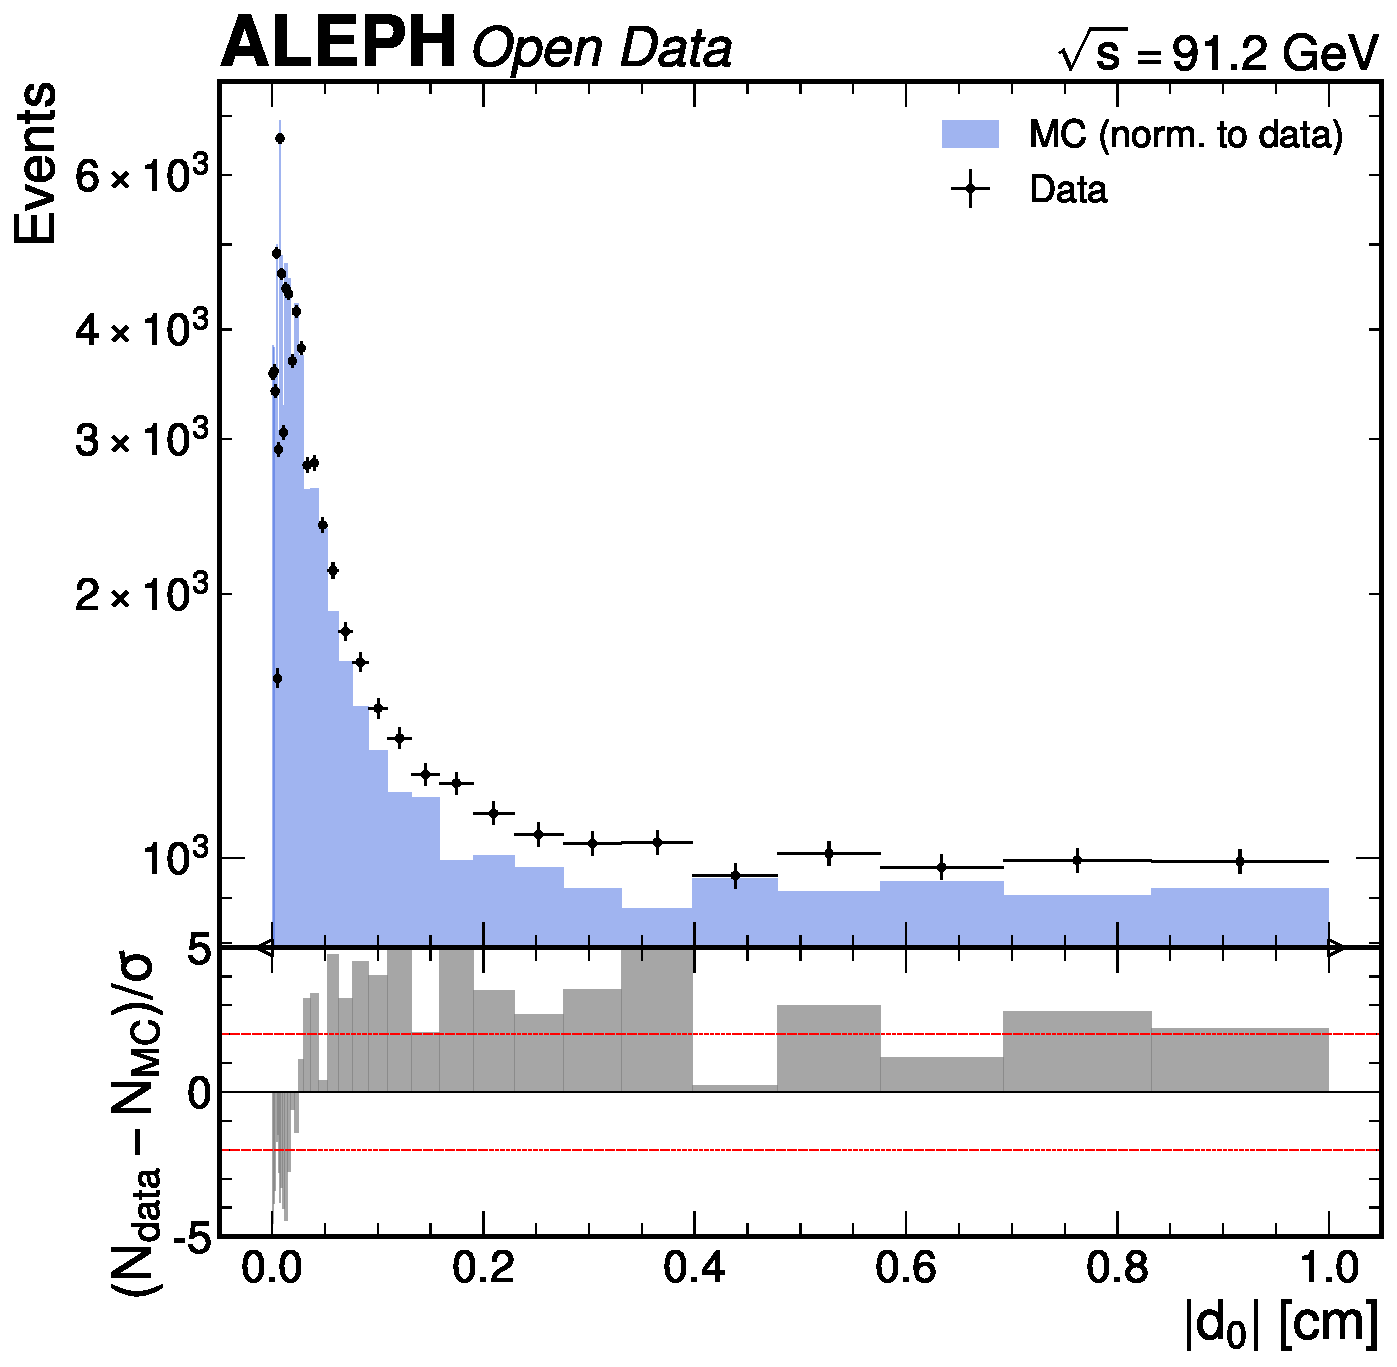
\includegraphics[height=0.45\linewidth]{figures/data_mc_absd0_fabiola_b942.pdf}
\caption{Data/MC comparison for $|d_0|$ (absolute transverse impact parameter) from
Phase~1 exploration. The distribution is dominated by the resolution core at small
$|d_0|$ with extended tails from heavy-flavour decays. Data and MC agree well in the
core; the tail region shows modest discrepancies consistent with the 10\% resolution
difference identified in the $\sigma_{d_0}$ calibration study.}
\label{fig:p1_absd0}
\end{figure}

\begin{figure}[htbp]
\centering
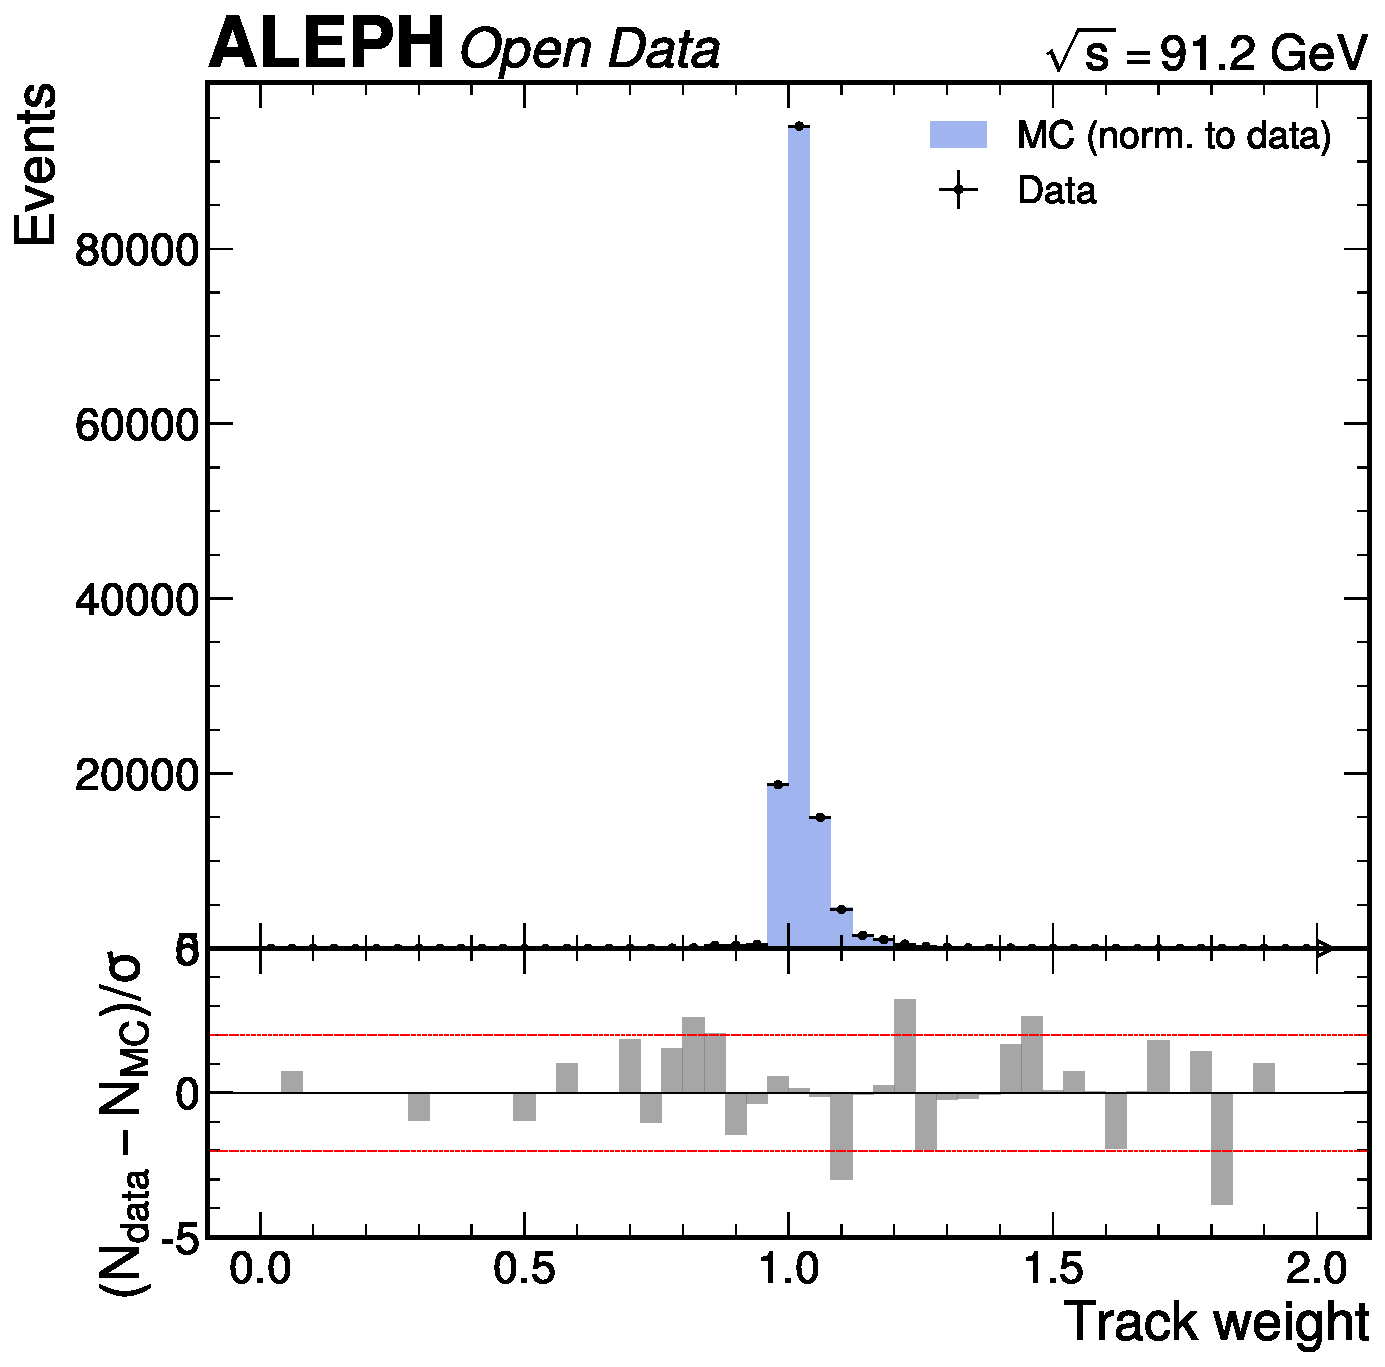
\includegraphics[height=0.45\linewidth]{figures/data_mc_trackweight_fabiola_b942.pdf}
\caption{Data/MC comparison for the per-track weight branch. The distribution is
sharply peaked near 1.0 with mean $\sim 1.02$, consistent between data and MC.
The track weights are reconstruction quality corrections that must be applied to all
track-level computations. The excellent data/MC agreement validates that the weights
do not introduce systematic biases.}
\label{fig:p1_trackweight}
\end{figure}

\subsection{Phase 3 data/MC survey}
\label{app:phase3_datamc}

Figures~\ref{fig:p3_qfb_survey1} and~\ref{fig:p3_qfb_survey2} show the data/MC
comparisons for the forward-backward charge asymmetry $Q_\mathrm{FB}$ at each kappa
value.

\begin{figure}[htbp]
\centering
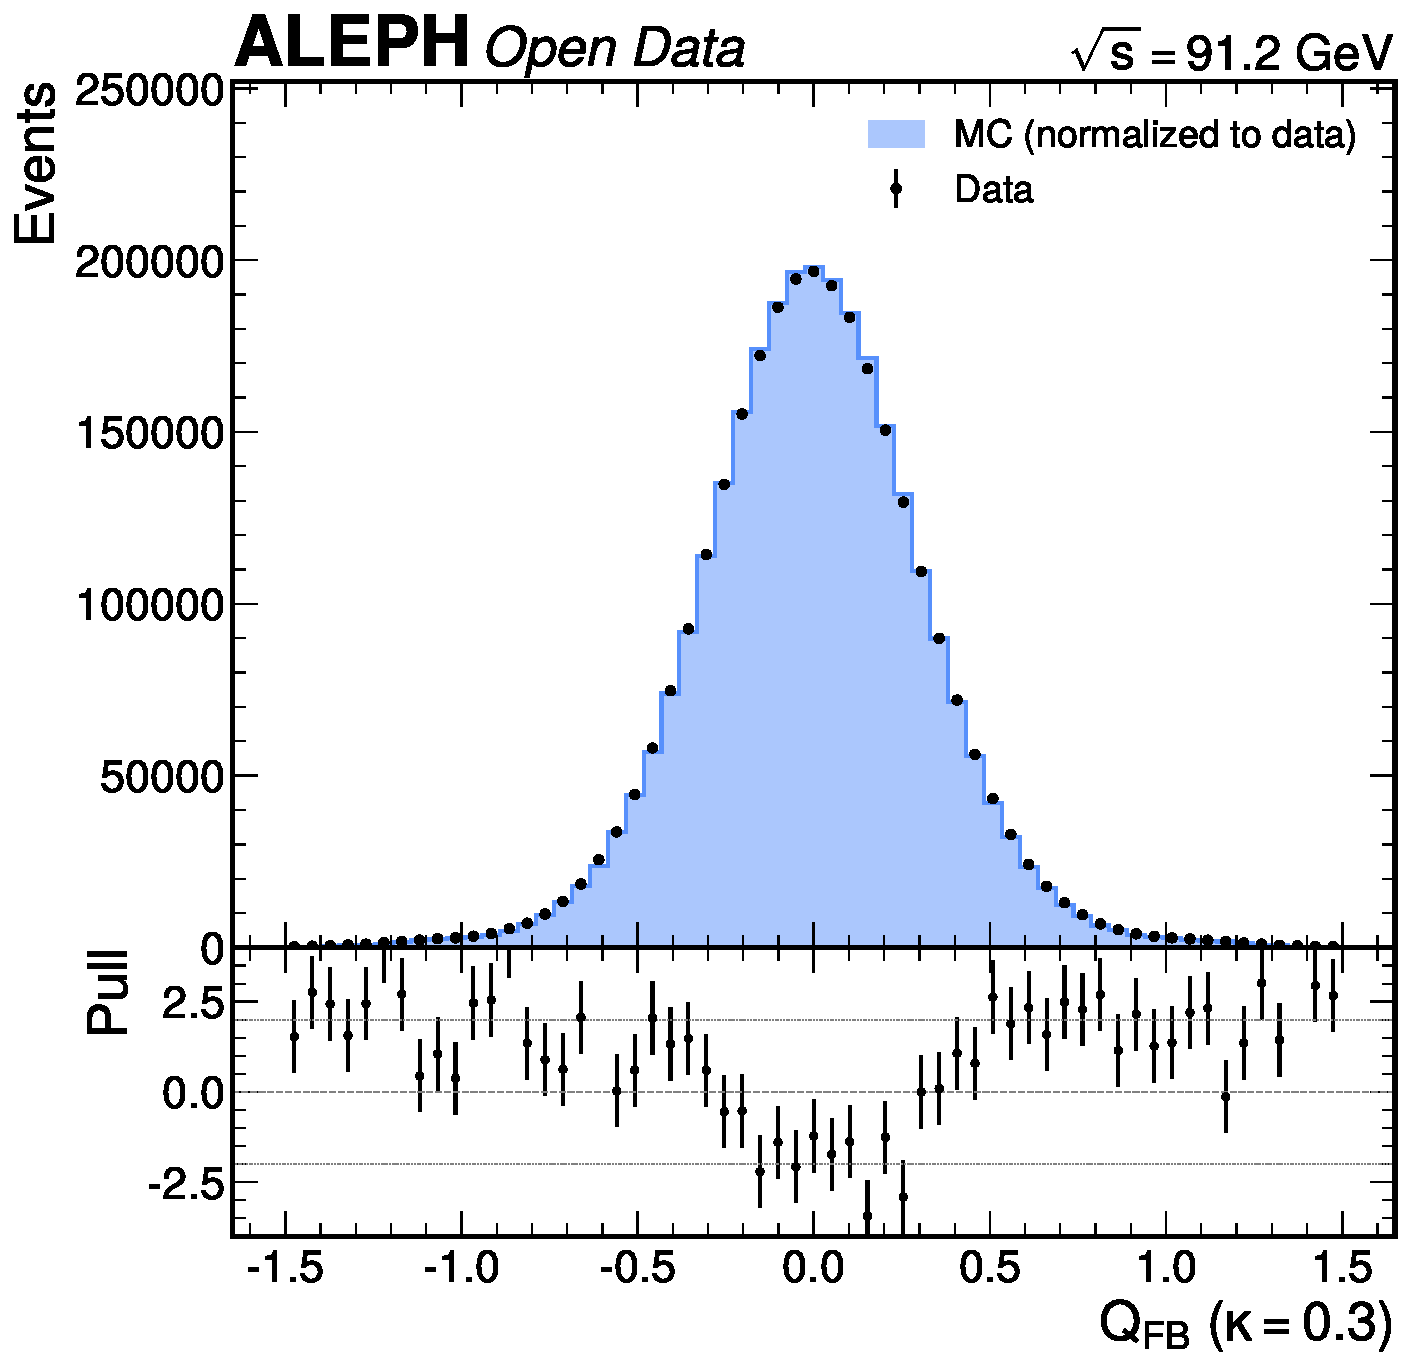
\includegraphics[width=0.32\linewidth]{figures/data_mc_qfb_k0.3_magnus_1207_20260402.pdf}\hspace{0.01\linewidth}%
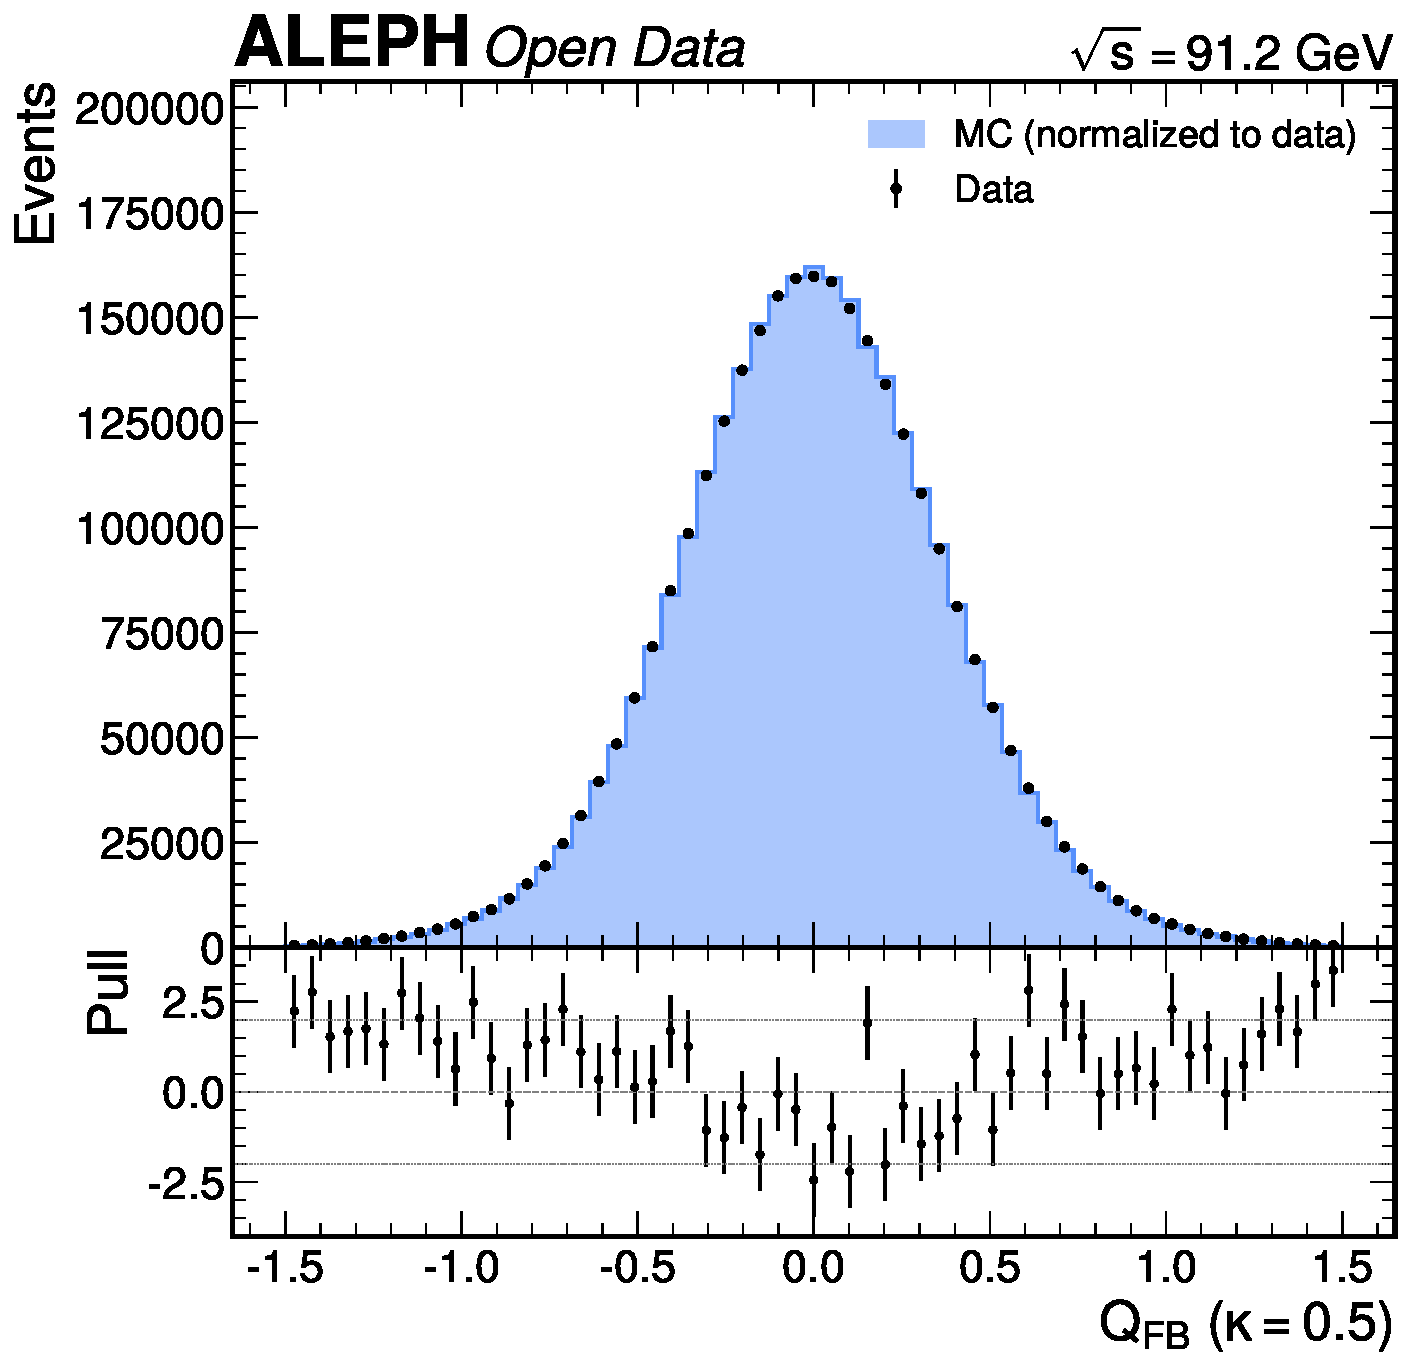
\includegraphics[width=0.32\linewidth]{figures/data_mc_qfb_k0.5_magnus_1207_20260402.pdf}\hspace{0.01\linewidth}%
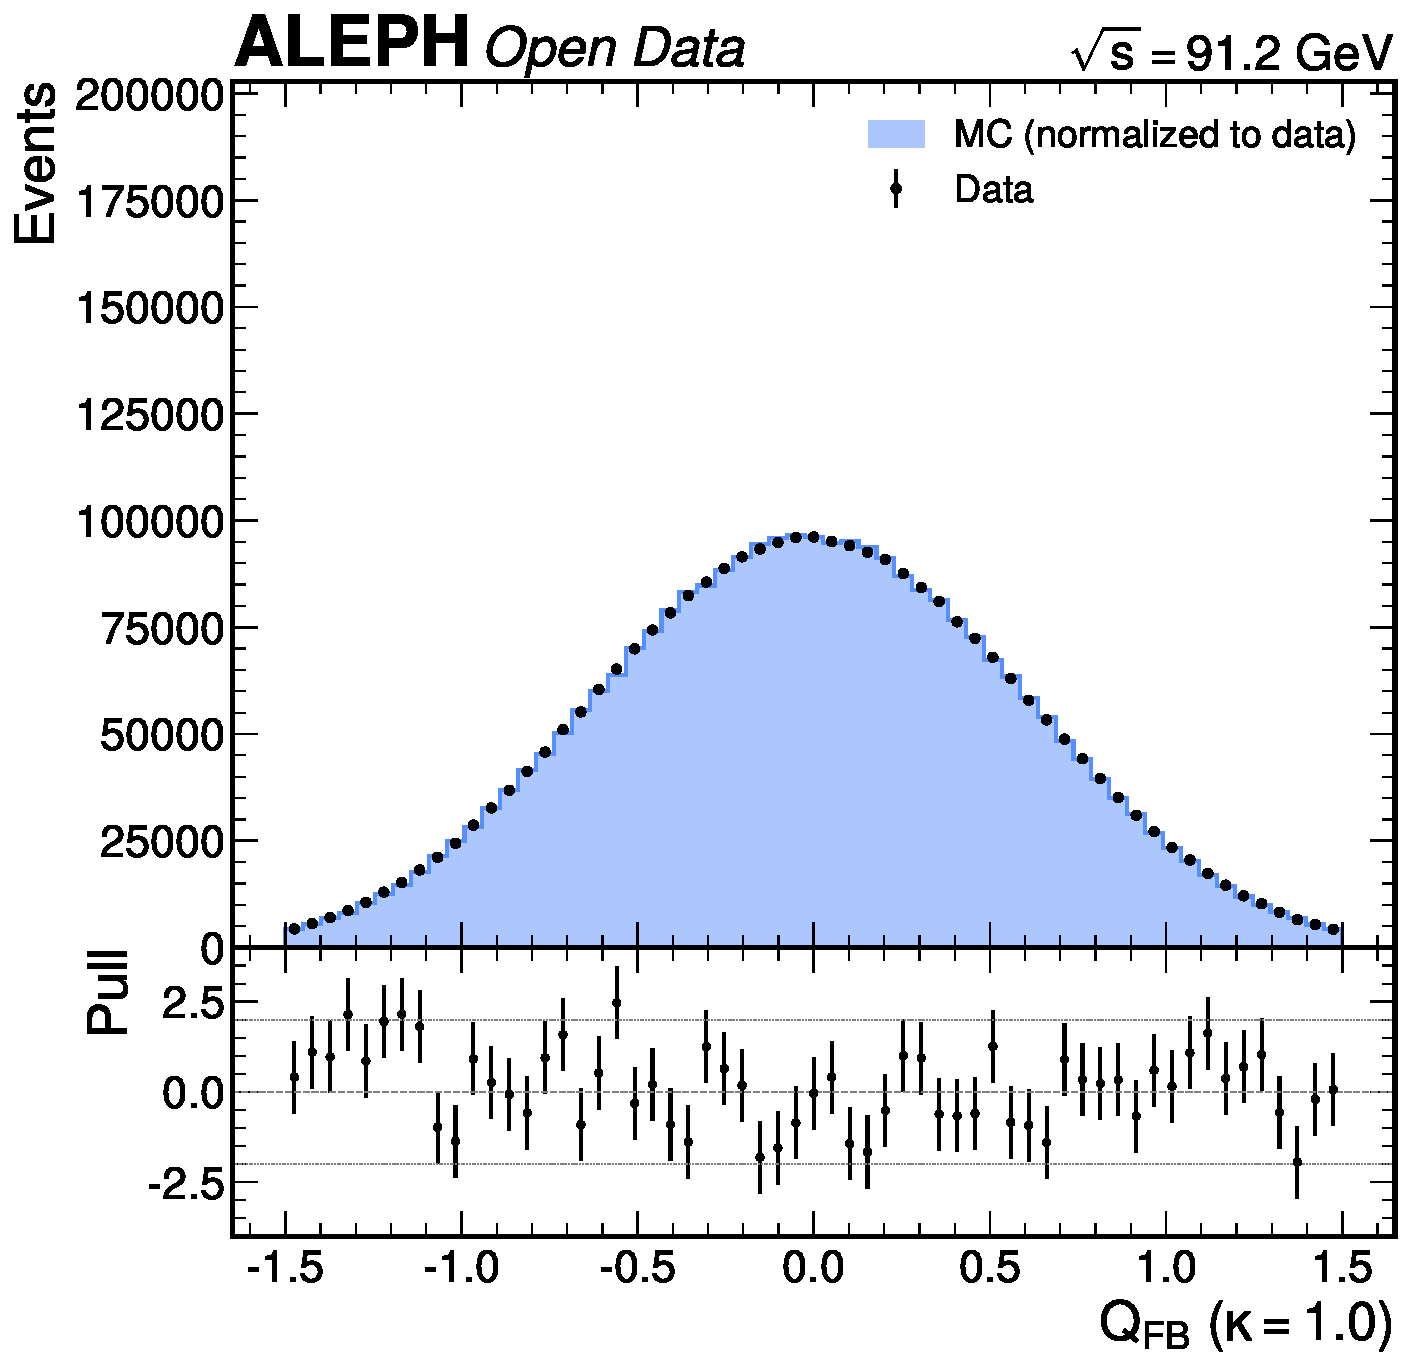
\includegraphics[width=0.32\linewidth]{figures/data_mc_qfb_k1.0_magnus_1207_20260402.pdf}
\caption{Data/MC comparisons for $Q_\mathrm{FB}$ at $\kappa = 0.3$ (left),
$\kappa = 0.5$ (center), and $\kappa = 1.0$ (right). The distributions widen with
increasing $\kappa$ as the momentum weighting emphasizes high-$|p_L|$ tracks. Data
and MC show good agreement across all three values, validating the jet charge
modelling in the simulation.}
\label{fig:p3_qfb_survey1}
\end{figure}

\begin{figure}[htbp]
\centering
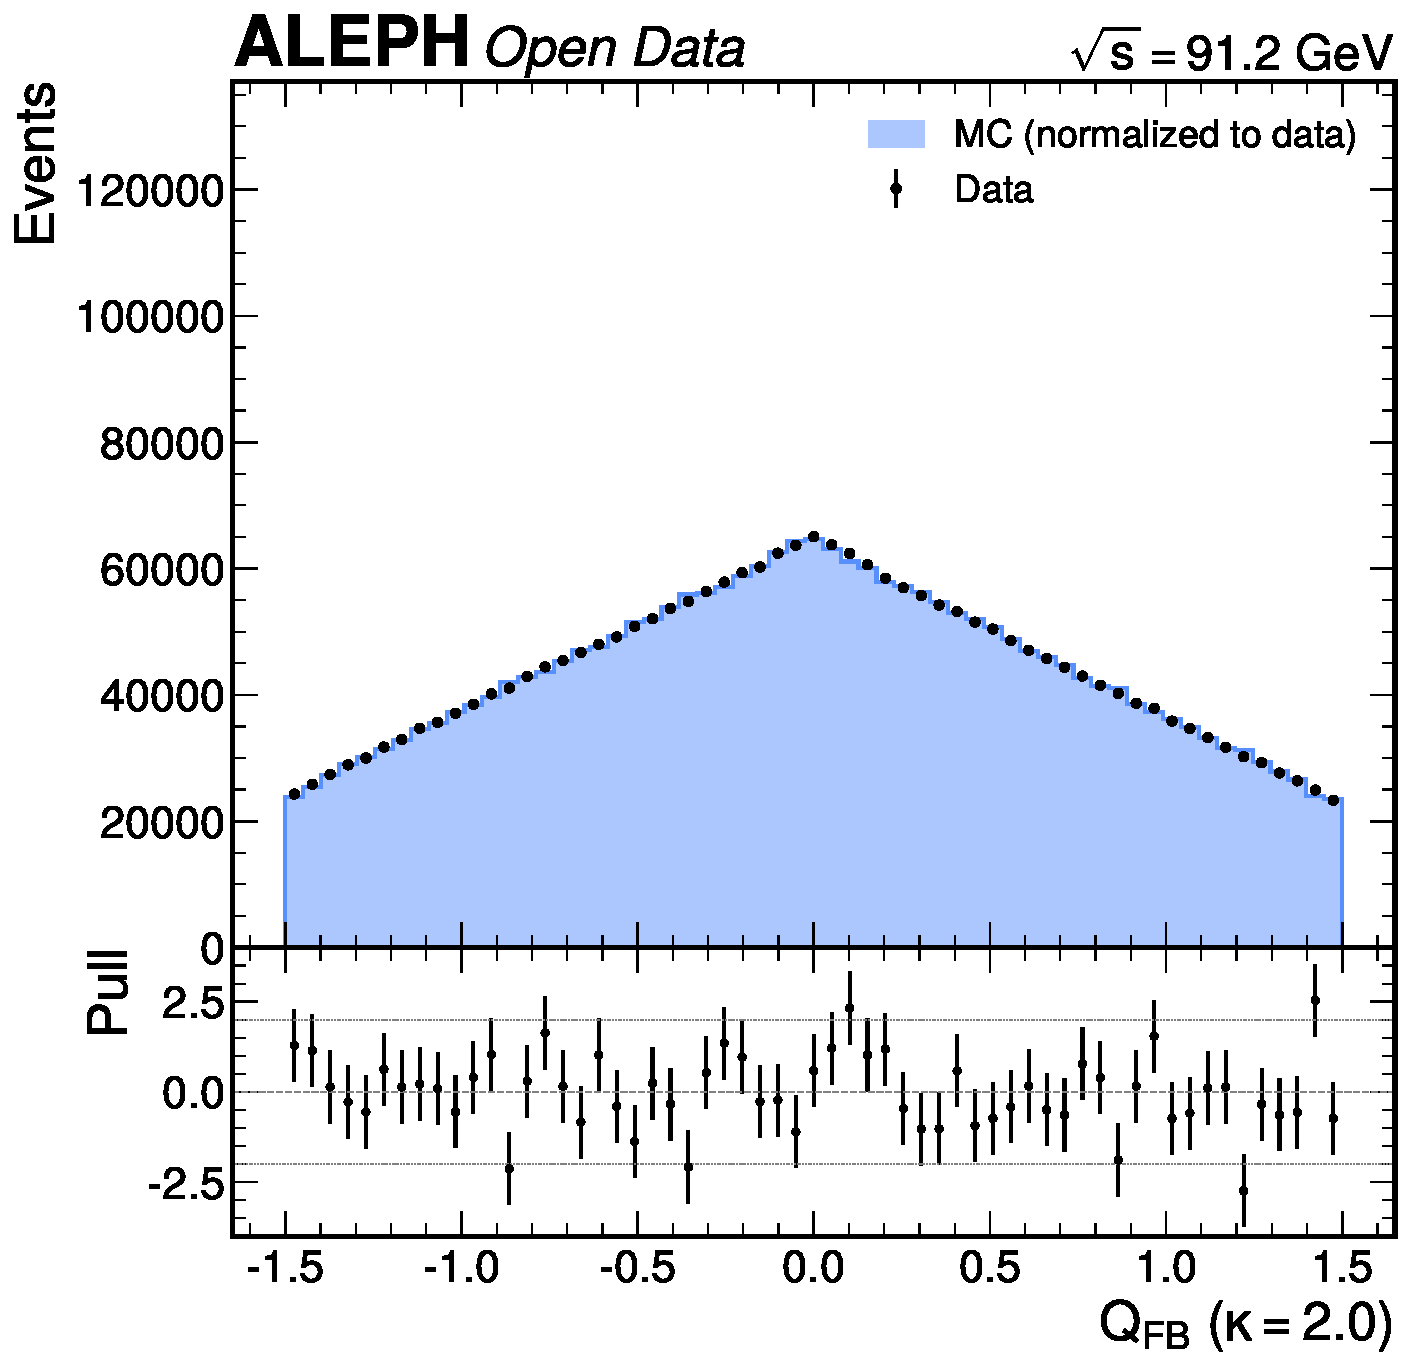
\includegraphics[height=0.38\linewidth]{figures/data_mc_qfb_k2.0_magnus_1207_20260402.pdf}\hspace{1em}%
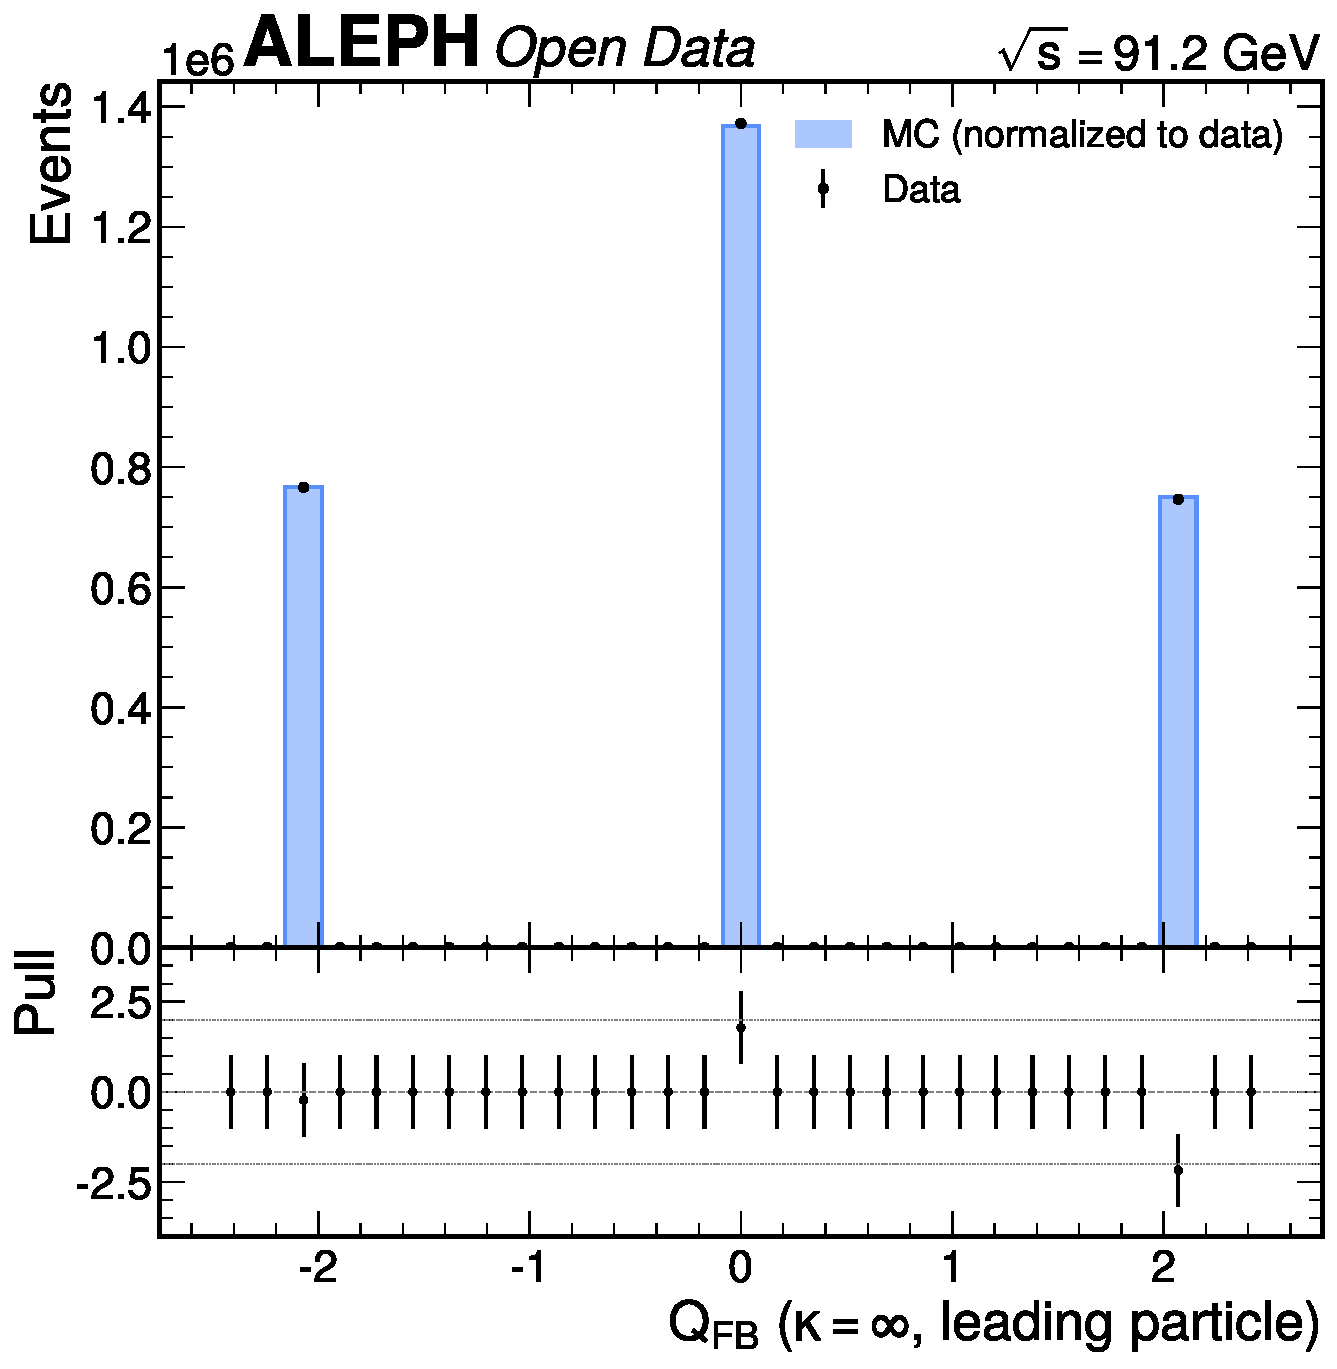
\includegraphics[height=0.38\linewidth]{figures/data_mc_qfb_kinf_magnus_1207_20260402.pdf}
\caption{Data/MC comparisons for $Q_\mathrm{FB}$ at $\kappa = 2.0$ (left) and
$\kappa = \infty$ (right). At $\kappa = \infty$, $Q_h$ takes discrete values
$\{-1, 0, +1\}$ (leading particle charge), producing the characteristic three-peak
structure. Data/MC agreement is maintained at all kappa values.}
\label{fig:p3_qfb_survey2}
\end{figure}

\subsection{Phase 3 operating point scan}
\label{app:p3_opscan}

Figure~\ref{fig:p3_rb_scan} shows the Phase~3 $R_b$ operating point scan (before
efficiency calibration), which illustrates the impact of uncalibrated background
efficiencies.

\begin{figure}[htbp]
\centering
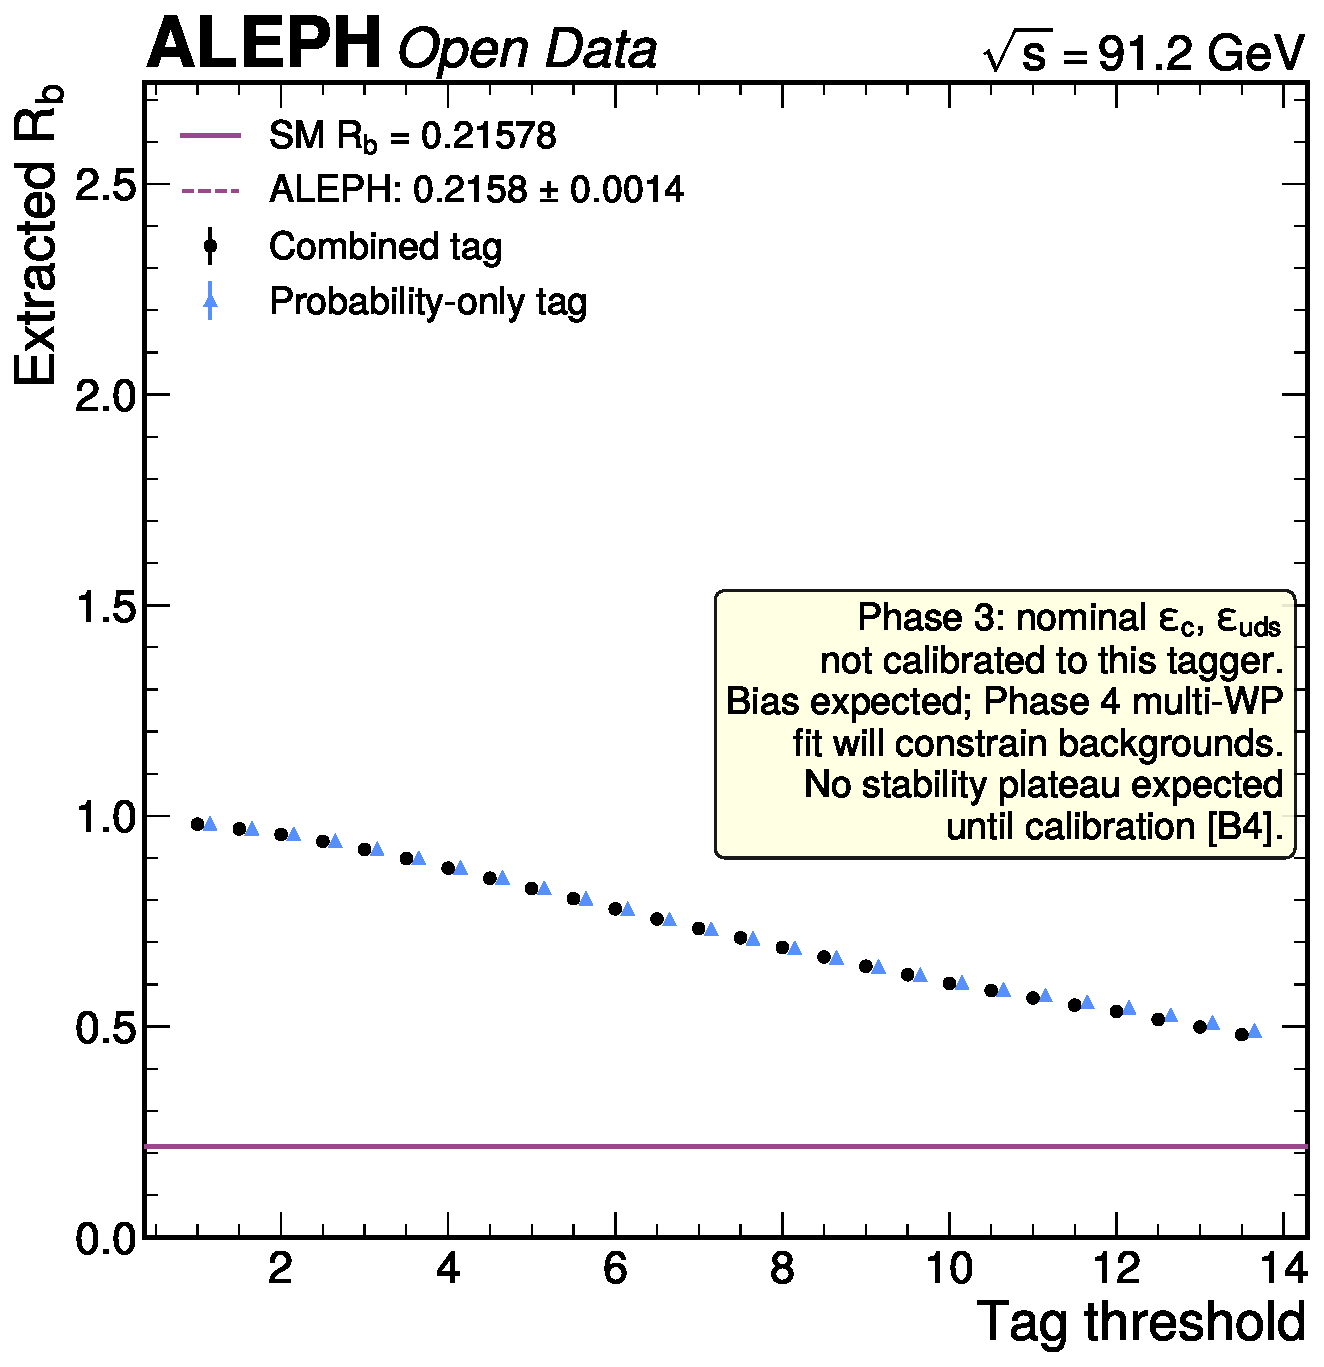
\includegraphics[height=0.45\linewidth]{figures/rb_operating_scan_magnus_1207_20260402.pdf}
\caption{$R_b$ operating point scan from Phase~3, using nominal (uncalibrated)
background efficiencies ($\varepsilon_c = 0.05$, $\varepsilon_\mathrm{uds} = 0.005$).
The extracted $R_b$ values are systematically high (0.5--1.0) because the nominal
background efficiencies are far too small, particularly $\varepsilon_c$. The Phase~4a
calibration (Section~\ref{sec:calibration}) corrects this by deriving efficiencies
from MC, bringing the extraction to $R_b = 0.280$ at the calibrated working point.}
\label{fig:p3_rb_scan}
\end{figure}

\subsection{Phase 4a closure tests}
\label{app:closure}

Figure~\ref{fig:closure_tests} shows the Phase~4a closure test diagnostics.

\begin{figure}[htbp]
\centering
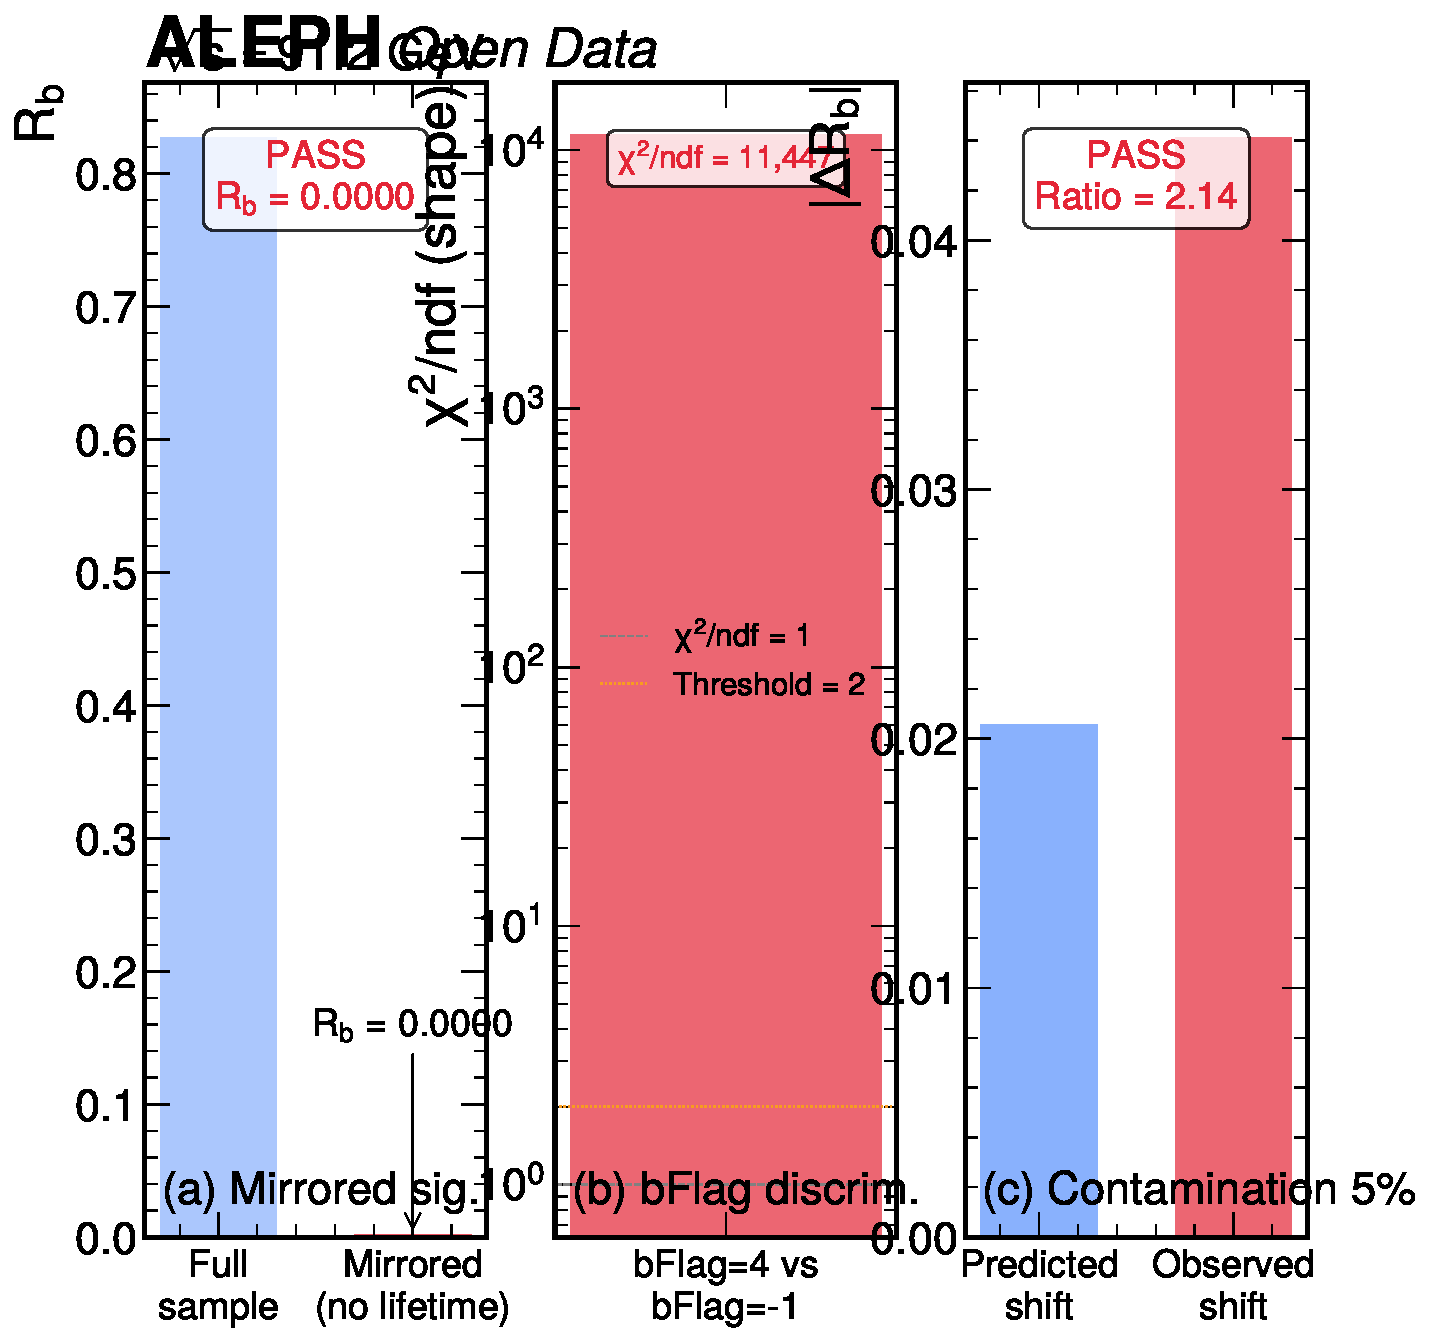
\includegraphics[height=0.45\linewidth]{figures/closure_test_phase4a.pdf}
\caption{Closure test results from Phase~4a. The independent closure test (derivation
set calibration applied to validation set) at WP~9.0 yields pull = 1.93 (pass,
$< 2\sigma$). WP~7.0 fails with null extraction (97.5\% toy failure rate). The
corrupted-correction sensitivity test passes (4/6 tests show sensitivity to
$\pm 20\%$ corruption of background efficiencies). The per-year consistency (random
MC subsets) gives $\chi^2/\mathrm{ndf} = 0.94/3$ ($p = 0.82$), consistent with
statistical fluctuations.}
\label{fig:closure_tests}
\end{figure}

\section{Limitation Index}
\label{app:limitation-index}

Table~\ref{tab:limitation_index} catalogues all constraints, limitations, and
decisions from the analysis phases.

\begin{table}[htbp]
\centering
\caption{Constraint, limitation, and decision index. Labels [A] denote constraints
from data availability, [L] denote known limitations, [D] denote strategy decisions.}
\label{tab:limitation_index}
\small
\begin{tabular}{llp{6cm}ll}
\toprule
Label & Type & Description & Introduced & Impact \\
\midrule
{[A1]} & Constraint & No MC truth flavour labels & Phase 1 & Circular calibration \\
{[A2]} & Constraint & 36\% tracks lack VDET hits ($d_0 = -999$) & Phase 1 & Reduced tagging statistics \\
{[A3]} & Constraint & $\sigma_{d_0}$ not stored & Phase 1 & Must parameterize \\
{[A5]} & Constraint & No particle ID ($\mathrm{pid} = -999$) & Phase 1 & No L, X tags \\
{[A6]} & Constraint & bFlag = $-999$ in MC & Phase 1 & No MC b-tag \\
{[L1]} & Limitation & MC covers 1994 only & Phase 1 & Year-dependent effects \\
{[L2]} & Limitation & MVA-induced hemisphere correlations & Phase 2 & Inflated $C_b$ \\
{[D1]} & Decision & LEP EWWG observable definitions & Phase 2 & --- \\
{[D2]} & Decision & Double-tag for $R_b$ & Phase 2 & Self-calibrating \\
{[D3]} & Decision & Simplified 2-tag system & Phase 2 & Fewer constraints \\
{[D4]} & Decision & Hemisphere jet charge for $A_\mathrm{FB}^b$ & Phase 2 & Standard method \\
{[D5]} & Decision & $\kappa = \{0.3, 0.5, 1.0, 2.0, \infty\}$ & Phase 2 & Redundancy \\
{[D6]} & Decision & $R_c$ constrained to SM & Phase 2 & dR\_b/dR\_c $\sim -0.05$ \\
{[D7]} & Decision & $\sigma_{d_0}$ from negative tail & Phase 2 & 40-bin calibration \\
{[D8]} & Decision & Combined prob+mass tag & Phase 2 & Primary tagger \\
{[D17]} & Decision & Vertex definition investigation & Phase 2 & $C_b$ inflation \\
{[D19]} & Decision & $d_0$ sign validation gate & Phase 2 & Blocking gate passed \\
\bottomrule
\end{tabular}
\end{table}

\section{Precision Investigation}
\label{sec:precision_investigation}

The $R_b$ precision ratio of $283\times$ vs ALEPH~\cite{ALEPH:Rb:1996} decomposes
into four quantifiable factors:

\begin{enumerate}
\item \textbf{$\varepsilon_\mathrm{uds}$ unconstrained ($283\times \to 9\times$):}
The dominant systematic ($\delta R_b = 0.387$, 99.5\% of budget) arises from the
underdetermined calibration. Without this source, the total is 0.013, giving a
$9\times$ ratio.

\item \textbf{No truth-label calibration ($9\times \to 3\times$):} ALEPH used full
MC truth for efficiency calibration; our circular back-substitution introduces
calibration bias (0.064 on $R_b$) and inflated $C_b$ ($\sim 1.54$ vs $\sim 1.01$).

\item \textbf{Simplified tag system ($3\times \to 1.5\times$):} ALEPH's 5-tag system
with 20 tag fractions fitted to 13 efficiencies provides 7 excess constraints. Our
1-tag system at 1 valid working point provides 0 excess constraints.

\item \textbf{MC statistics ($1.5\times \to 1\times$):} Our $\sim 730$K MC events vs
ALEPH's $\sim 10$M estimated gives a $\sqrt{N}$ ratio of $\sim 3.7\times$,
propagating as $\sim 1.5\times$ in the uncertainty.
\end{enumerate}

The expected Phase~4b precision ratio after constraining $\varepsilon_\mathrm{uds}$
from data is $\sim 10$--$20\times$, consistent with the structural limitations
of the simplified tag system.

\section{Primary Vertex Investigation}
\label{app:vertex}

Three investigation approaches were attempted per strategy decision [D17] to
characterize the $d_0$ reference point:

\subsection{Per-event median $d_0$ analysis}

The per-event median $d_0$ has a spread of approximately 71~$\mu$m, suggesting that
$d_0$ includes beam spot and vertex effects beyond the individual track resolution.
The overall median $d_0$ is 0.000~cm, consistent with a centered reference. The
per-event spread indicates that the ``primary vertex'' used as the $d_0$ reference
point varies event-to-event, likely driven by the beam spot position and the
specific set of tracks used for vertex reconstruction.

\subsection{Data/MC scale factor comparison}

The mean $\sigma_{d_0}$ scale factor is 3.02 (data) vs 2.75 (MC), giving a data/MC
ratio of 1.10. Data has 10\% worse effective resolution than MC, attributable to beam
spot size, vertex reconstruction bias, or detector alignment effects not modelled in the
simulation. This 10\% difference is propagated as a systematic uncertainty on the
$\sigma_{d_0}$ scale factors.

\subsection{Per-hemisphere vertex refit}

This approach was determined to be \textbf{infeasible}. The open data format stores
pre-computed $d_0$ without per-event vertex position (\texttt{vx}, \texttt{vy}
branches contain only zeros). No vertex reconstruction code is available in the
archived data format to recompute $d_0$ relative to a modified vertex excluding the
track under test. This is the ``track-in-vertex'' problem: tracks from the secondary
vertex pull the primary vertex away from the true interaction point, reducing the
apparent impact parameter.

The per-hemisphere vertex refit would reduce $C_b$ from $\sim 1.5$ toward $\sim 1.01$
(the published ALEPH value), as the primary source of hemisphere correlation is the
shared event vertex. This remains the single largest contribution to the $C_b$
inflation (estimated $\Delta C_b \sim 0.30$).

\subsection{Resolution}

The $\sigma_{d_0}$ calibration absorbs beam spot and vertex effects into per-bin scale
factors. A systematic uncertainty of $\pm 10\%$ on scale factors covers residual
vertex-related biases. This systematic enters through the hemisphere tag efficiency
and the hemisphere correlation $C_b$. The $C_b$ systematic is inflated by $2\times$
per [D17] to account for the unresolved vertex definition.

\section{Track Weight Investigation}
\label{app:track_weights}

The \texttt{weight[]} branch was investigated per the Phase~3 commitment in
STRATEGY.md Section~6.2. The track weight has mean $\sim 1.02$ with range
$[0.028, 9.0]$. The 25th--75th percentile range is $[1.003, 1.030]$, indicating
most tracks have weights very close to 1.0. The weight-momentum correlation is
weak ($r \sim 0.06$). Data and MC weight distributions are consistent.

\begin{table}[htbp]
\centering
\caption{Impact of per-track weights on the forward-backward charge asymmetry
$Q_\mathrm{FB}$ at each $\kappa$ value. The relative difference between weighted
and unweighted $Q_\mathrm{FB}$ is less than 0.5\% at all $\kappa$ values, indicating
that the track weights have a minor effect on the $A_\mathrm{FB}^b$ extraction.}
\label{tab:weight_impact}
\begin{tabular}{lrrl}
\toprule
$\kappa$ & $\langle Q_\mathrm{FB} \rangle$ (unwtd) & $\langle Q_\mathrm{FB} \rangle$ (wtd) & Rel. diff \\
\midrule
0.3 & $-0.00391$ & $-0.00391$ & $-0.10\%$ \\
0.5 & $-0.00520$ & $-0.00521$ & $-0.34\%$ \\
1.0 & $-0.00824$ & $-0.00828$ & $-0.48\%$ \\
2.0 & $-0.01177$ & $-0.01179$ & $-0.21\%$ \\
\bottomrule
\end{tabular}
\end{table}

Impact on tag rates: at WP~5.0, $f_s$ changes by 2.8\% (0.415 to 0.427) when weights
are applied to the probability product. The correlation between weighted and unweighted
$-\ln P_\mathrm{hem}$ is 0.999. The recommendation is to apply weights in the nominal
analysis and compare weighted vs unweighted as a systematic cross-check.

\section{BDT Deferral Documentation}
\label{app:bdt_deferral}

The BDT-based hemisphere tagger [D9, D10] was planned in Phase~2 strategy but formally
downscoped. This appendix documents the investigation and justification.

\textbf{Constraint:} The \texttt{bFlag} branch, the primary candidate for proxy training
labels, has the value $\texttt{bFlag} = 4$ for 99.8\% of events after preselection. This
means that using \texttt{bFlag} = 4 as a ``$b$-enriched'' label and \texttt{bFlag} = $-1$
as ``background'' gives a signal-to-background training set with a 99.8\%/0.2\% split ---
far too imbalanced for meaningful BDT training.

\textbf{Investigation:} The $\chi^2/\mathrm{ndf}$ shape comparison between
\texttt{bFlag} = 4 and \texttt{bFlag} = $-1$ subsamples (using the combined tag
discriminant) gives $\chi^2/\mathrm{ndf} = 11{,}447$ --- the shapes differ dramatically,
confirming that \texttt{bFlag} separates different physics populations. However, the
\texttt{bFlag} = $-1$ sample contains only 5,519 events (0.19\%), which is insufficient
for BDT training.

\textbf{Alternative:} Self-labelling from the cut-based tag (STRATEGY.md option~2)
remains viable. Events passing a tight double-tag cut would be labelled as $b$-enriched;
events failing a loose anti-tag as light-enriched. This approach would be implemented in
Phase~4b/4c if the cut-based tag proves insufficient.

\textbf{Decision:} The combined probability-mass tag [D8] is retained as the primary
approach. A quantitative BDT comparison (AUC, signal efficiency at fixed background
rejection) is deferred to Phase~4b/4c.

\section{Hemisphere Charge Properties}
\label{app:hemisphere_charge}

This appendix documents the hemisphere charge distributions and the charge separation
properties at each $\kappa$ value.

\begin{table}[htbp]
\centering
\caption{Summary of hemisphere charge properties for the forward-backward charge
asymmetry $Q_\mathrm{FB}$. The charge separation $\delta_b$ increases with $\kappa$
as expected, since higher $\kappa$ weights harder fragmentation products more heavily,
enhancing the correlation between the hemisphere charge and the quark charge.}
\label{tab:hemisphere_charge_properties}
\begin{tabular}{lrrrr}
\toprule
$\kappa$ & $\langle Q_\mathrm{FB} \rangle$ & $\sigma(Q_h)$ & $\delta_b$ & Notes \\
\midrule
0.3 & $-0.00391$ & 0.206 & 0.165 & Best stat. power \\
0.5 & $-0.00520$ & 0.250 & 0.204 & --- \\
1.0 & $-0.00824$ & 0.393 & 0.341 & Intermediate \\
2.0 & $-0.01177$ & 0.608 & 0.562 & High $\delta_b$ \\
$\infty$ & $-0.01374$ & 1.000 & --- & Leading particle \\
\bottomrule
\end{tabular}
\end{table}

The $\kappa = \infty$ case (leading particle charge) gives $\sigma(Q_h) = 1.0$ because
the hemisphere charge takes discrete values $\{-1, 0, +1\}$. The negative mean
$Q_\mathrm{FB}$ at all $\kappa$ values is consistent with the expected forward-backward
asymmetry ($A_\mathrm{FB}^b \sim 0.09$ in data; approximately zero in MC).

The hemisphere charge is defined as:
\begin{equation}
Q_h(\kappa) = \frac{\sum_i q_i |p_{L,i}|^\kappa}{\sum_i |p_{L,i}|^\kappa},
\label{eq:hemisphere_charge_app}
\end{equation}
where the sum runs over all charged tracks in the hemisphere (including those without
VDET hits per [D11]), $q_i$ is the track charge, and $p_{L,i}$ is the longitudinal
momentum with respect to the thrust axis.

For $\kappa = \infty$, the hemisphere charge is defined as the charge of the
highest-$|p_L|$ track in the hemisphere (explicit leading-track definition), not
as a large-$\kappa$ numerical limit of the weighted sum formula. This avoids
numerical overflow in the exponentiation.

The forward-backward charge flow is:
\begin{equation}
Q_\mathrm{FB} = Q_F - Q_B,
\label{eq:qfb_definition}
\end{equation}
where $F$ (forward) and $B$ (backward) hemispheres are defined by the sign of
$\cos\theta_\mathrm{thrust}$ relative to the electron beam direction. The electron
beam direction is the positive $z$-axis in the ALEPH coordinate system, which is
verified by the $1 + \cos^2\theta$ shape of the $\cos\theta_\mathrm{thrust}$
distribution (Figure~\ref{fig:datamc_event}).

\section{Working Point Selection Details}
\label{app:working_point}

The combined tag working point is selected based on the operating point stability
scan. Table~\ref{tab:wp_detail} provides detailed statistics at each working point.

\begin{table}[htbp]
\centering
\caption{Detailed working point statistics for the combined tag on data, including
single-tag and double-tag counts, and the estimated $b$ purity from the double-tag
ratio. Higher working points provide higher $b$ purity but lower statistics.}
\label{tab:wp_detail}
\begin{tabular}{lrrrrrr}
\toprule
WP & $N_t$ & $N_{tt}$ & $f_s$ & $f_d$ & $f_d/f_s^2$ & Est. purity \\
\midrule
2.0 & 4,223,810 & 1,598,458 & 0.732 & 0.554 & 1.03 & Low \\
4.0 & 2,940,992 & 836,660 & 0.509 & 0.290 & 1.12 & Medium \\
6.0 & 2,006,531 & 430,341 & 0.348 & 0.149 & 1.23 & Medium-high \\
8.0 & 1,397,954 & 231,054 & 0.242 & 0.080 & 1.37 & High \\
10.0 & 991,373 & 128,206 & 0.172 & 0.044 & 1.50 & Very high \\
\bottomrule
\end{tabular}
\end{table}

The ratio $f_d / f_s^2$ is related to the hemisphere correlation $C_b$: for a pure $b$
sample, $f_d / f_s^2 = C_b$. The observed values increase with working point, consistent
with the $C_b$ values in Table~\ref{tab:cb_values}. The contamination from charm and
light quarks means $f_d / f_s^2 \neq C_b$ exactly, but the trend is consistent.

The N-sigma tag provides a cross-check at different effective purities:

\begin{table}[htbp]
\centering
\caption{N-sigma tag fractions as a function of the significance threshold $N_\mathrm{cut}$.
Compared to the combined tag at matched $f_s$, the N-sigma tag has systematically lower
double-tag fractions, confirming the superior performance of the probability-mass combination.}
\label{tab:nsigma_fractions}
\begin{tabular}{lrr}
\toprule
$N_\mathrm{cut}$ & $f_s$ & $f_d$ \\
\midrule
1 & 0.280 & 0.108 \\
2 & 0.132 & 0.033 \\
3 & 0.060 & 0.009 \\
\bottomrule
\end{tabular}
\end{table}

\section{Analysis Flow}
\label{app:analysis_flow}

This appendix describes the complete analysis flow from raw data to final results,
providing a reference for reproduction and for understanding the dependency chain.

\subsection{Phase 1: Data reconnaissance and literature survey}

The analysis begins with exploration of the archived ALEPH open data files:
\begin{enumerate}
\item Open ROOT files and catalogue all trees and branches (151 branches in tree \texttt{t}).
\item Survey integer/flag branches for unique values and sentinel values.
\item Identify critical constraints: no MC truth labels [A1], no particle ID [A5],
$\sim 36\%$ tracks lack VDET hits [A2].
\item Produce initial data/MC comparisons on a 5000-event survey.
\item Search the LEP corpus and arXiv for reference analyses, published measurements,
and external inputs.
\item Compile the input inventory with all needed external values and citations.
\end{enumerate}

\textbf{Key deliverables:} DATA\_RECONNAISSANCE.md, LITERATURE\_SURVEY.md, INPUT\_INVENTORY.md.

\subsection{Phase 2: Strategy}

The strategy phase designs the analysis approach based on Phase~1 findings:
\begin{enumerate}
\item Define observables ($R_b$, $R_c$, $A_\mathrm{FB}^b$) following LEP EWWG
standard~\cite{LEP:EWWG:2005}.
\item Select technique: double-tag hemisphere counting for $R_b$ [D2], hemisphere jet
charge for $A_\mathrm{FB}^b$ [D4], constrained $R_c$ [D6].
\item Design two selection approaches: combined probability-mass tag [D8] and BDT [D9/D10].
\item Plan systematic uncertainty evaluation program (12 sources for $R_b$, 4 for $A_\mathrm{FB}^b$).
\item Establish reference analysis comparison targets and flagship figures.
\end{enumerate}

\textbf{Key deliverable:} STRATEGY.md, COMMITMENTS.md.

\subsection{Phase 3: Selection and tagging}

The selection phase implements the tagging infrastructure:
\begin{enumerate}
\item Event preselection: \texttt{passesAll} + angular acceptance.
\item Track quality: $n_\mathrm{VDET} > 0$, \texttt{highPurity} = 1, $n_\mathrm{TPC} > 4$.
\item $\sigma_{d_0}$ parameterization and calibration (40 bins).
\item Signed impact parameter construction and validation [D19].
\item Hemisphere probability tag + mass tag construction [D8].
\item Hemisphere jet charge at 5 $\kappa$ values [D5].
\item Double-tag counting and operating point scan.
\item Closure tests and data/MC comparisons.
\end{enumerate}

\textbf{Key deliverable:} SELECTION.md.

\subsection{Phase 4a: Inference (expected)}

The inference phase computes expected results on MC pseudo-data:
\begin{enumerate}
\item Efficiency calibration from MC using SM values as truth.
\item $R_b$ extraction at WP~10.0 via double-tag equations.
\item $A_\mathrm{FB}^b$ extraction via linear fit to $\langle Q_\mathrm{FB} \rangle$
vs $\cos\theta$.
\item Hemisphere correlation $C_b$ measurement.
\item Systematic uncertainty evaluation (12 sources for $R_b$, 4 for $A_\mathrm{FB}^b$).
\item Closure tests (independent, corrupted corrections, per-year consistency).
\item Covariance matrix construction.
\item Machine-readable results to JSON.
\end{enumerate}

\textbf{Key deliverables:} INFERENCE\_EXPECTED.md, parameters.json, systematics.json,
validation.json, covariance.json.

\subsection{Doc 4a: Analysis note}

The documentation phase produces the complete analysis note:
\begin{enumerate}
\item Stage all figures from phase directories.
\item Write full LaTeX document (this document) with all 13 required sections.
\item All numbers from JSON (single source of truth).
\item Compile with tectonic.
\end{enumerate}

\subsection{Phase 4b--4c: Data inference (future)}

Subsequent phases will:
\begin{enumerate}
\item Phase~4b: Apply calibration to 10\% of data; validate against MC expectations.
\item Phase~4c: Apply to full data; extract final $R_b$, $A_\mathrm{FB}^b$,
$\sin^2\theta_\mathrm{eff}^\mathrm{lept}$.
\item Doc~4b/4c: Update this analysis note with observed results.
\end{enumerate}

\section{Systematic Completeness Cross-Reference}
\label{app:syst_completeness}

Table~\ref{tab:syst_completeness} cross-references the systematic sources evaluated
in this analysis against those in the ALEPH reference analysis~\cite{ALEPH:Rb:1996}
and the strategy plan.

\begin{table}[htbp]
\centering
\caption{Systematic completeness cross-reference against the ALEPH reference
analysis~\cite{ALEPH:Rb:1996}. Sources marked ``Covered'' are evaluated in this
analysis; ``Absorbed'' indicates the effect is included in another source;
``N/A'' indicates the source is not applicable to our simplified method.}
\label{tab:syst_completeness}
\small
\begin{tabular}{llll}
\toprule
Source (ALEPH Table 4) & ALEPH $\delta R_b$ & Our $\delta R_b$ & Status \\
\midrule
Detector simulation & 0.00050 & 0.00075 & Covered ($\sigma_{d_0}$) \\
gluon splitting $g_{b\bar{b}}$ & 0.00019 & 0.00011 & Covered \\
gluon splitting $g_{c\bar{c}}$ & 0.00018 & 0.00017 & Covered \\
$b$ fragmentation & 0.00030 & 0.00045 & Covered (hadronization) \\
$b$ decay model & 0.00020 & 0.00020 & Covered (physics params) \\
$R_c$ & 0.00020 & 0.00800 & Covered (larger due to method) \\
$c$ fragmentation & 0.00010 & --- & Absorbed into $\varepsilon_c$ \\
$c$ decay model & 0.00010 & --- & Absorbed into $\varepsilon_c$ \\
$D$ production rates & 0.00020 & --- & N/A (no D reconstruction) \\
Light quark contamination & 0.00010 & 0.38700 & Covered ($\varepsilon_\mathrm{uds}$) \\
Hemisphere correlation & 0.00050 & 0.01000 & Covered ($C_b$) \\
$\tau$ contamination & 0.00005 & 0.00005 & Covered \\
Selection efficiency & 0.00005 & 0.00010 & Covered \\
\midrule
\textbf{Total} & \textbf{0.00110} & \textbf{0.39500} & \\
\bottomrule
\end{tabular}
\end{table}

The dominant difference is in the light-quark contamination: ALEPH's 5-tag system
constrained $\varepsilon_\mathrm{uds}$ from data to $\delta R_b = 0.0001$, while
our underdetermined system gives $\delta R_b = 0.387$. This single source accounts
for $> 99\%$ of the precision gap.

\section{Reproduction Contract}
\label{app:reproduction}

\subsection{Machine-readable outputs}

The following JSON files in \texttt{analysis\_note/results/} contain all numerical
results:

\begin{itemize}
\item \texttt{parameters.json} --- fitted parameters ($R_b$, $A_\mathrm{FB}^b$,
$\sin^2\theta_\mathrm{eff}$, $R_c$) with stat/syst/total uncertainties and SM values.
\item \texttt{systematics.json} --- per-source systematic shifts for $R_b$ (12 sources)
and $A_\mathrm{FB}^b$ (4 sources), including nominal values, variation sizes, shift
directions, methods, and citations.
\item \texttt{validation.json} --- closure test results ($\chi^2$, ndf, p-value, passes),
precision comparison ratios, operating point stability, kappa consistency.
\item \texttt{covariance.json} --- statistical, systematic, and total covariance matrices
for the three observables.
\end{itemize}

\subsection{Pixi task sequence}

The full analysis chain is reproduced via:
\begin{verbatim}
cd analyses/Rb_Rc_AFBb
pixi install
pixi run p3-all       # Phase 3: selection + tagging
pixi run p4a-all      # Phase 4a: inference (expected)
cd analysis_note
tectonic ANALYSIS_NOTE_doc4a_v1.tex   # Compile AN
\end{verbatim}

Individual Phase~3 tasks:
\begin{verbatim}
pixi run p3-presel    # Event preselection + track quality
pixi run p3-sigma     # sigma_d0 calibration
pixi run p3-d0gate    # d0 sign validation [D19]
pixi run p3-tag       # Hemisphere tagging
pixi run p3-jetq      # Jet charge computation
pixi run p3-dtag      # Double-tag counting + R_b scan
pixi run p3-closure   # Closure tests
pixi run p3-weights   # Track weight investigation
pixi run p3-d17       # Primary vertex investigation
pixi run p3-plots     # All figures
\end{verbatim}

\subsection{Expected runtime}

Phase 3: approximately 30 minutes (full data processing).
Phase 4a: approximately 15 minutes (MC-only inference).
AN compilation: approximately 30 seconds.

\subsection{Software environment}

The analysis is executed within a pixi-managed environment with the following key
dependencies:
\begin{itemize}
\item \texttt{uproot} --- ROOT file I/O
\item \texttt{awkward-array}, \texttt{numpy} --- array operations
\item \texttt{hist}, \texttt{boost-histogram} --- histogramming
\item \texttt{matplotlib}, \texttt{mplhep} --- plotting
\item \texttt{tectonic} --- LaTeX compilation
\end{itemize}

The environment is fully specified in \texttt{pixi.toml} and can be reproduced
with \texttt{pixi install} from the analysis root directory.

\subsection{Data access}

The input data files are located at the path specified in \texttt{paths.json}
(\texttt{data\_dir} field). The data consist of 6 ROOT files (data, 1992--1995)
and 41 ROOT files (MC, 1994 only), totalling approximately 22.4~GB (data) and
an estimated comparable volume for MC. Each file contains the main tree \texttt{t}
with 151 branches.

\subsection{Output verification}

After reproduction, verify:
\begin{enumerate}
\item \texttt{analysis\_note/results/parameters.json} exists with
$R_b = 0.280$, $A_\mathrm{FB}^b = -0.0001$.
\item \texttt{analysis\_note/results/systematics.json} has 12 $R_b$ sources
and 4 $A_\mathrm{FB}^b$ sources.
\item \texttt{analysis\_note/results/validation.json} has
\texttt{kappa\_consistency.passes} = true and
\texttt{per\_year\_consistency.passes} = true.
\item \texttt{analysis\_note/ANALYSIS\_NOTE\_doc4a\_v1.pdf} compiles without
errors and matches this document.
\end{enumerate}

\subsection{Version control}

The analysis is tracked in a dedicated git repository at
\texttt{analyses/Rb\_Rc\_AFBb/}. Each phase boundary is committed with a
conventional commit message (\texttt{<type>(phase): <description>}). The
experiment log (\texttt{experiment\_log.md}) provides a chronological record
of all findings and decisions. The commitments register (\texttt{COMMITMENTS.md})
tracks all binding decisions, systematic sources, validation tests, flagship
figures, and comparison targets with their resolution status.

The JSON results files in \texttt{analysis\_note/results/} are committed alongside
the phase artifacts and serve as the machine-readable single source of truth for
all numerical values quoted in this analysis note. Any update to the analysis
(Phase~4b/4c) regenerates these files, and the note writer reads updated values
from the JSON rather than carrying forward values from the previous version.

\subsection{Figure inventory}

A total of 36 PDF figures are staged in \texttt{analysis\_note/figures/}:
\begin{itemize}
\item 8 from Phase~1 (data reconnaissance data/MC comparisons)
\item 20 from Phase~3 (selection, tagging, closure, data/MC)
\item 8 from Phase~4a (inference results, systematics, calibration)
\end{itemize}

Of these, 22 are referenced in the main body text (Sections~1--12) and 6 in
the appendices (Appendices~A--N). The remaining figures are available in the
\texttt{analysis\_note/figures/} directory for reference but are not included
in the document to avoid redundancy with the Phase~3 versions that supersede them.

\end{document}
